%!TEX TS-program = xelatex
% NOTE: as of 17 Sept 2012, this compiles in xelatex

\documentclass[10pt]{beamer}
\usepackage{etoolbox}
\makeatletter
\patchcmd{\slideentry}{\ifnum#2>0}{\ifnum2>0}{}{\@error{unable to patch}}
\makeatother

\usetheme{Frankfurt}

%\setbeamertemplate{footline}[page number]
%\setbeamercovered{transparent}
\setbeamercovered{invisible}
% To remove the navigation symbols from 
% the bottom of slides%
\setbeamertemplate{navigation symbols}{} 
%\setbeamercovered{transparent}
%\usecolortheme{albatross}
%\usecolortheme{beetle}
%\usecolortheme{crane}
%\usecolortheme{dove}
%\usecolortheme{fly}
%\usecolortheme{seagull}
%\usecolortheme{wolverine}
%\usecolortheme{beaver} % I like this one
%
\usepackage{coordsys} % for number lines
\usepackage{graphicx}
\usepackage{multirow}
\usepackage{caption}
\usepackage{subfig}
\usepackage{tikz}
%\usepackage{bm}         % For typesetting bold math (not \mathbold)
%\logo{\includegraphics[height=0.6cm]{yourlogo.eps}}
%

% font customization
% \usepackage{mathspec}
% \usepackage{xunicode}
% \usepackage{xltxtra}
% \setmainfont{Gill Sans}
% \setmathsfont(Digits,Latin,Greek){Gill Sans}

%%%%%%%%%%%%%%%%%%%%%%%%%%%%%%%%%%%%%%%%%
\title[Regime Classification \hspace{14em} \insertframenumber/
\inserttotalframenumber]{Probabilistic Measures of \\ Regime Type}
\author{MADCOW Project}
% \institute[Duke University]
% {
% {\emph{sfm12@duke.edu}} \\
% \medskip
% Duke University 
% }
\date{\today}

% \graphicspath{{/Users/janus829/Dropbox/Research/wardprojects/regimeclassif/}}

\begin{document}

%%%%%%%%%%%%%%%%%%%%%%%%%%%%%%%%%%%%%%%%%
\begin{frame}
\titlepage
\end{frame}
%%%%%%%%%%%%%%%%%%%%%%%%%%%%%%%%%%%%%%%%%

\section{Labeled Data}

%%%%%%%%%%%%%%%%%%%%%%%%%%%%%%%%%%%%%%%%%
\begin{frame}
\frametitle{Distributions of Polity at Various Cuts}

\begin{figure}[ht]
	\centering
	\resizebox{1\textwidth}{!}{% Created by tikzDevice version 0.7.0 on 2014-11-07 12:14:32
% !TEX encoding = UTF-8 Unicode
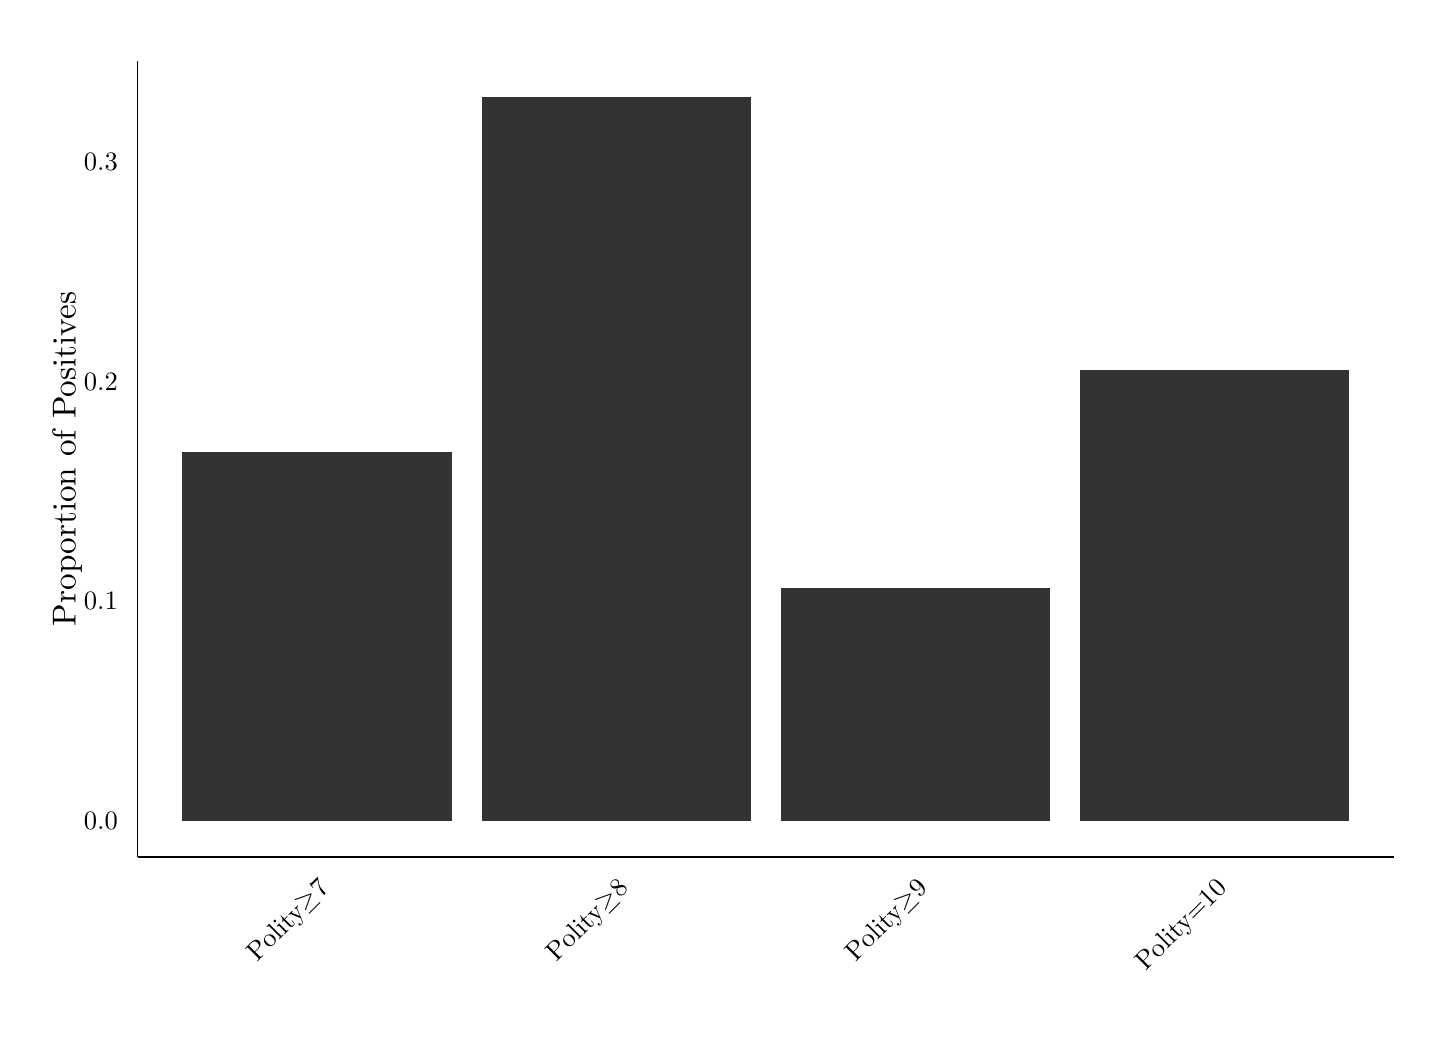
\begin{tikzpicture}[x=1pt,y=1pt]
\definecolor[named]{fillColor}{rgb}{1.00,1.00,1.00}
\path[use as bounding box,fill=fillColor,fill opacity=0.00] (0,0) rectangle (505.89,361.35);
\begin{scope}
\path[clip] (  0.00,  0.00) rectangle (505.89,361.35);
\definecolor[named]{drawColor}{rgb}{1.00,1.00,1.00}
\definecolor[named]{fillColor}{rgb}{1.00,1.00,1.00}

\path[draw=drawColor,line width= 0.6pt,line join=round,line cap=round,fill=fillColor] (  0.00,  0.00) rectangle (505.89,361.35);
\end{scope}
\begin{scope}
\path[clip] ( 39.69, 61.79) rectangle (493.85,349.30);
\definecolor[named]{fillColor}{rgb}{1.00,1.00,1.00}

\path[fill=fillColor] ( 39.69, 61.79) rectangle (493.85,349.31);
\definecolor[named]{fillColor}{rgb}{0.20,0.20,0.20}

\path[fill=fillColor] ( 55.91, 74.86) rectangle (153.23,208.01);

\path[fill=fillColor] (164.04, 74.86) rectangle (261.36,336.24);

\path[fill=fillColor] (272.17, 74.86) rectangle (369.49,158.70);

\path[fill=fillColor] (380.31, 74.86) rectangle (477.63,237.60);
\end{scope}
\begin{scope}
\path[clip] (  0.00,  0.00) rectangle (505.89,361.35);
\definecolor[named]{drawColor}{rgb}{0.00,0.00,0.00}

\path[draw=drawColor,line width= 0.6pt,line join=round] ( 39.69, 61.79) --
	( 39.69,349.30);
\end{scope}
\begin{scope}
\path[clip] (  0.00,  0.00) rectangle (505.89,361.35);
\definecolor[named]{drawColor}{rgb}{0.00,0.00,0.00}

\node[text=drawColor,anchor=base east,inner sep=0pt, outer sep=0pt, scale=  0.96] at ( 32.57, 71.55) {0.0};

\node[text=drawColor,anchor=base east,inner sep=0pt, outer sep=0pt, scale=  0.96] at ( 32.57,150.95) {0.1};

\node[text=drawColor,anchor=base east,inner sep=0pt, outer sep=0pt, scale=  0.96] at ( 32.57,230.35) {0.2};

\node[text=drawColor,anchor=base east,inner sep=0pt, outer sep=0pt, scale=  0.96] at ( 32.57,309.75) {0.3};
\end{scope}
\begin{scope}
\path[clip] (  0.00,  0.00) rectangle (505.89,361.35);
\definecolor[named]{drawColor}{rgb}{0.00,0.00,0.00}

\path[draw=drawColor,line width= 0.6pt,line join=round] ( 39.69, 61.79) --
	(493.85, 61.79);
\end{scope}
\begin{scope}
\path[clip] (  0.00,  0.00) rectangle (505.89,361.35);
\definecolor[named]{drawColor}{rgb}{0.00,0.00,0.00}

\node[text=drawColor,rotate= 45.00,anchor=base east,inner sep=0pt, outer sep=0pt, scale=  0.96] at (109.24, 50.00) {Polity$\geq$7};

\node[text=drawColor,rotate= 45.00,anchor=base east,inner sep=0pt, outer sep=0pt, scale=  0.96] at (217.37, 50.00) {Polity$\geq$8};

\node[text=drawColor,rotate= 45.00,anchor=base east,inner sep=0pt, outer sep=0pt, scale=  0.96] at (325.51, 50.00) {Polity$\geq$9};

\node[text=drawColor,rotate= 45.00,anchor=base east,inner sep=0pt, outer sep=0pt, scale=  0.96] at (433.64, 50.00) {Polity$=$10};
\end{scope}
\begin{scope}
\path[clip] (  0.00,  0.00) rectangle (505.89,361.35);
\definecolor[named]{drawColor}{rgb}{0.00,0.00,0.00}

\node[text=drawColor,rotate= 90.00,anchor=base,inner sep=0pt, outer sep=0pt, scale=  1.20] at ( 17.30,205.55) {Proportion of Positives};
\end{scope}
\end{tikzpicture}
}	
\end{figure}

\end{frame}
%%%%%%%%%%%%%%%%%%%%%%%%%%%%%%%%%%%%%%%%%

\section{SVM Probability Distribution}

%%%%%%%%%%%%%%%%%%%%%%%%%%%%%%%%%%%%%%%%%
% Distributions
\begin{frame}
\frametitle{Distribution of SVM Probabilities from 2012 Predictions}

\begin{figure}[ht]
	\centering
	\resizebox{1\textwidth}{!}{% Created by tikzDevice version 0.6.2 on 2014-10-03 02:50:04
% !TEX encoding = UTF-8 Unicode
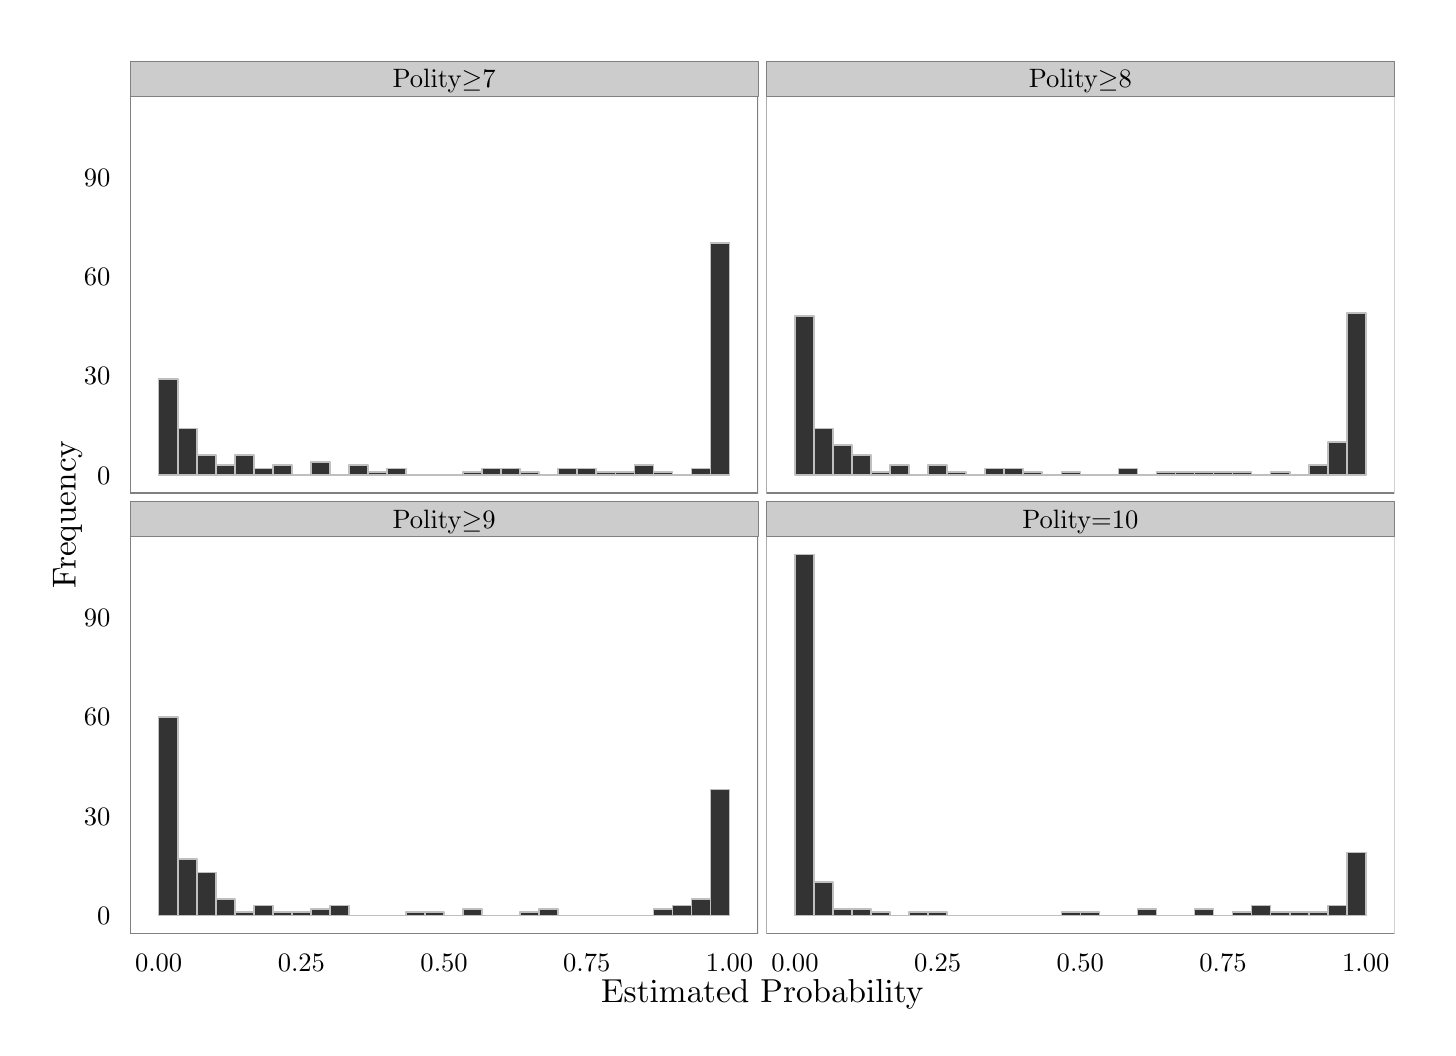
\begin{tikzpicture}[x=1pt,y=1pt]
\definecolor[named]{drawColor}{rgb}{0.00,0.00,0.00}
\definecolor[named]{fillColor}{rgb}{1.00,1.00,1.00}
\fill[color=fillColor,fill opacity=0.00,] (0,0) rectangle (505.89,361.35);
\begin{scope}
\path[clip] (  0.00,  0.00) rectangle (505.89,361.35);
\end{scope}
\begin{scope}
\path[clip] (  0.00,  0.00) rectangle (505.89,361.35);
\end{scope}
\begin{scope}
\path[clip] (  0.00,  0.00) rectangle (505.89,361.35);
\definecolor[named]{drawColor}{rgb}{1.00,1.00,1.00}
\definecolor[named]{fillColor}{rgb}{1.00,1.00,1.00}

\draw[color=drawColor,line width= 0.6pt,line cap=round,line join=round,fill=fillColor,] (  0.00,  0.00) rectangle (505.89,361.35);
\end{scope}
\begin{scope}
\path[clip] (  0.00,  0.00) rectangle (505.89,361.35);
\end{scope}
\begin{scope}
\path[clip] ( 37.02,193.18) rectangle (263.93,336.67);
\definecolor[named]{fillColor}{rgb}{1.00,1.00,1.00}

\draw[fill=fillColor,draw opacity=0.00,] ( 37.02,193.18) rectangle (263.93,336.67);
\definecolor[named]{drawColor}{rgb}{0.75,0.75,0.75}
\definecolor[named]{fillColor}{rgb}{0.20,0.20,0.20}

\draw[color=drawColor,line width= 0.6pt,line join=round,fill=fillColor,] ( 47.33,199.70) rectangle ( 54.21,234.40);

\draw[color=drawColor,line width= 0.6pt,line join=round,fill=fillColor,] ( 54.21,199.70) rectangle ( 61.09,216.45);

\draw[color=drawColor,line width= 0.6pt,line join=round,fill=fillColor,] ( 61.09,199.70) rectangle ( 67.96,206.88);

\draw[color=drawColor,line width= 0.6pt,line join=round,fill=fillColor,] ( 67.96,199.70) rectangle ( 74.84,203.29);

\draw[color=drawColor,line width= 0.6pt,line join=round,fill=fillColor,] ( 74.84,199.70) rectangle ( 81.71,206.88);

\draw[color=drawColor,line width= 0.6pt,line join=round,fill=fillColor,] ( 81.71,199.70) rectangle ( 88.59,202.09);

\draw[color=drawColor,line width= 0.6pt,line join=round,fill=fillColor,] ( 88.59,199.70) rectangle ( 95.47,203.29);

\draw[color=drawColor,line width= 0.6pt,line join=round,fill=fillColor,] ( 95.47,199.70) rectangle (102.34,199.70);

\draw[color=drawColor,line width= 0.6pt,line join=round,fill=fillColor,] (102.34,199.70) rectangle (109.22,204.49);

\draw[color=drawColor,line width= 0.6pt,line join=round,fill=fillColor,] (109.22,199.70) rectangle (116.09,199.70);

\draw[color=drawColor,line width= 0.6pt,line join=round,fill=fillColor,] (116.09,199.70) rectangle (122.97,203.29);

\draw[color=drawColor,line width= 0.6pt,line join=round,fill=fillColor,] (122.97,199.70) rectangle (129.85,200.89);

\draw[color=drawColor,line width= 0.6pt,line join=round,fill=fillColor,] (129.85,199.70) rectangle (136.72,202.09);

\draw[color=drawColor,line width= 0.6pt,line join=round,fill=fillColor,] (136.72,199.70) rectangle (143.60,199.70);

\draw[color=drawColor,line width= 0.6pt,line join=round,fill=fillColor,] (143.60,199.70) rectangle (150.47,199.70);

\draw[color=drawColor,line width= 0.6pt,line join=round,fill=fillColor,] (150.47,199.70) rectangle (157.35,199.70);

\draw[color=drawColor,line width= 0.6pt,line join=round,fill=fillColor,] (157.35,199.70) rectangle (164.23,200.89);

\draw[color=drawColor,line width= 0.6pt,line join=round,fill=fillColor,] (164.23,199.70) rectangle (171.10,202.09);

\draw[color=drawColor,line width= 0.6pt,line join=round,fill=fillColor,] (171.10,199.70) rectangle (177.98,202.09);

\draw[color=drawColor,line width= 0.6pt,line join=round,fill=fillColor,] (177.98,199.70) rectangle (184.85,200.89);

\draw[color=drawColor,line width= 0.6pt,line join=round,fill=fillColor,] (184.85,199.70) rectangle (191.73,199.70);

\draw[color=drawColor,line width= 0.6pt,line join=round,fill=fillColor,] (191.73,199.70) rectangle (198.61,202.09);

\draw[color=drawColor,line width= 0.6pt,line join=round,fill=fillColor,] (198.61,199.70) rectangle (205.48,202.09);

\draw[color=drawColor,line width= 0.6pt,line join=round,fill=fillColor,] (205.48,199.70) rectangle (212.36,200.89);

\draw[color=drawColor,line width= 0.6pt,line join=round,fill=fillColor,] (212.36,199.70) rectangle (219.23,200.89);

\draw[color=drawColor,line width= 0.6pt,line join=round,fill=fillColor,] (219.23,199.70) rectangle (226.11,203.29);

\draw[color=drawColor,line width= 0.6pt,line join=round,fill=fillColor,] (226.11,199.70) rectangle (232.99,200.89);

\draw[color=drawColor,line width= 0.6pt,line join=round,fill=fillColor,] (232.99,199.70) rectangle (239.86,199.70);

\draw[color=drawColor,line width= 0.6pt,line join=round,fill=fillColor,] (239.86,199.70) rectangle (246.74,202.09);

\draw[color=drawColor,line width= 0.6pt,line join=round,fill=fillColor,] (246.74,199.70) rectangle (253.61,283.47);
\definecolor[named]{drawColor}{rgb}{0.50,0.50,0.50}

\draw[color=drawColor,line width= 0.6pt,line cap=round,line join=round,fill opacity=0.00,] ( 37.02,193.18) rectangle (263.93,336.67);
\end{scope}
\begin{scope}
\path[clip] (  0.00,  0.00) rectangle (505.89,361.35);
\end{scope}
\begin{scope}
\path[clip] (266.94,193.18) rectangle (493.85,336.67);
\definecolor[named]{fillColor}{rgb}{1.00,1.00,1.00}

\draw[fill=fillColor,draw opacity=0.00,] (266.94,193.18) rectangle (493.85,336.67);
\definecolor[named]{drawColor}{rgb}{0.75,0.75,0.75}
\definecolor[named]{fillColor}{rgb}{0.20,0.20,0.20}

\draw[color=drawColor,line width= 0.6pt,line join=round,fill=fillColor,] (277.25,199.70) rectangle (284.13,257.14);

\draw[color=drawColor,line width= 0.6pt,line join=round,fill=fillColor,] (284.13,199.70) rectangle (291.00,216.45);

\draw[color=drawColor,line width= 0.6pt,line join=round,fill=fillColor,] (291.00,199.70) rectangle (297.88,210.47);

\draw[color=drawColor,line width= 0.6pt,line join=round,fill=fillColor,] (297.88,199.70) rectangle (304.76,206.88);

\draw[color=drawColor,line width= 0.6pt,line join=round,fill=fillColor,] (304.76,199.70) rectangle (311.63,200.89);

\draw[color=drawColor,line width= 0.6pt,line join=round,fill=fillColor,] (311.63,199.70) rectangle (318.51,203.29);

\draw[color=drawColor,line width= 0.6pt,line join=round,fill=fillColor,] (318.51,199.70) rectangle (325.38,199.70);

\draw[color=drawColor,line width= 0.6pt,line join=round,fill=fillColor,] (325.38,199.70) rectangle (332.26,203.29);

\draw[color=drawColor,line width= 0.6pt,line join=round,fill=fillColor,] (332.26,199.70) rectangle (339.14,200.89);

\draw[color=drawColor,line width= 0.6pt,line join=round,fill=fillColor,] (339.14,199.70) rectangle (346.01,199.70);

\draw[color=drawColor,line width= 0.6pt,line join=round,fill=fillColor,] (346.01,199.70) rectangle (352.89,202.09);

\draw[color=drawColor,line width= 0.6pt,line join=round,fill=fillColor,] (352.89,199.70) rectangle (359.76,202.09);

\draw[color=drawColor,line width= 0.6pt,line join=round,fill=fillColor,] (359.76,199.70) rectangle (366.64,200.89);

\draw[color=drawColor,line width= 0.6pt,line join=round,fill=fillColor,] (366.64,199.70) rectangle (373.52,199.70);

\draw[color=drawColor,line width= 0.6pt,line join=round,fill=fillColor,] (373.52,199.70) rectangle (380.39,200.89);

\draw[color=drawColor,line width= 0.6pt,line join=round,fill=fillColor,] (380.39,199.70) rectangle (387.27,199.70);

\draw[color=drawColor,line width= 0.6pt,line join=round,fill=fillColor,] (387.27,199.70) rectangle (394.14,199.70);

\draw[color=drawColor,line width= 0.6pt,line join=round,fill=fillColor,] (394.14,199.70) rectangle (401.02,202.09);

\draw[color=drawColor,line width= 0.6pt,line join=round,fill=fillColor,] (401.02,199.70) rectangle (407.90,199.70);

\draw[color=drawColor,line width= 0.6pt,line join=round,fill=fillColor,] (407.90,199.70) rectangle (414.77,200.89);

\draw[color=drawColor,line width= 0.6pt,line join=round,fill=fillColor,] (414.77,199.70) rectangle (421.65,200.89);

\draw[color=drawColor,line width= 0.6pt,line join=round,fill=fillColor,] (421.65,199.70) rectangle (428.52,200.89);

\draw[color=drawColor,line width= 0.6pt,line join=round,fill=fillColor,] (428.52,199.70) rectangle (435.40,200.89);

\draw[color=drawColor,line width= 0.6pt,line join=round,fill=fillColor,] (435.40,199.70) rectangle (442.28,200.89);

\draw[color=drawColor,line width= 0.6pt,line join=round,fill=fillColor,] (442.28,199.70) rectangle (449.15,199.70);

\draw[color=drawColor,line width= 0.6pt,line join=round,fill=fillColor,] (449.15,199.70) rectangle (456.03,200.89);

\draw[color=drawColor,line width= 0.6pt,line join=round,fill=fillColor,] (456.03,199.70) rectangle (462.90,199.70);

\draw[color=drawColor,line width= 0.6pt,line join=round,fill=fillColor,] (462.90,199.70) rectangle (469.78,203.29);

\draw[color=drawColor,line width= 0.6pt,line join=round,fill=fillColor,] (469.78,199.70) rectangle (476.66,211.67);

\draw[color=drawColor,line width= 0.6pt,line join=round,fill=fillColor,] (476.66,199.70) rectangle (483.53,258.34);
\definecolor[named]{drawColor}{rgb}{0.50,0.50,0.50}

\draw[color=drawColor,line width= 0.6pt,line cap=round,line join=round,fill opacity=0.00,] (266.94,193.18) rectangle (493.85,336.67);
\end{scope}
\begin{scope}
\path[clip] (  0.00,  0.00) rectangle (505.89,361.35);
\end{scope}
\begin{scope}
\path[clip] ( 37.02, 34.03) rectangle (263.93,177.53);
\definecolor[named]{fillColor}{rgb}{1.00,1.00,1.00}

\draw[fill=fillColor,draw opacity=0.00,] ( 37.02, 34.03) rectangle (263.93,177.53);
\definecolor[named]{drawColor}{rgb}{0.75,0.75,0.75}
\definecolor[named]{fillColor}{rgb}{0.20,0.20,0.20}

\draw[color=drawColor,line width= 0.6pt,line join=round,fill=fillColor,] ( 47.33, 40.56) rectangle ( 54.21,112.36);

\draw[color=drawColor,line width= 0.6pt,line join=round,fill=fillColor,] ( 54.21, 40.56) rectangle ( 61.09, 60.90);

\draw[color=drawColor,line width= 0.6pt,line join=round,fill=fillColor,] ( 61.09, 40.56) rectangle ( 67.96, 56.12);

\draw[color=drawColor,line width= 0.6pt,line join=round,fill=fillColor,] ( 67.96, 40.56) rectangle ( 74.84, 46.54);

\draw[color=drawColor,line width= 0.6pt,line join=round,fill=fillColor,] ( 74.84, 40.56) rectangle ( 81.71, 41.75);

\draw[color=drawColor,line width= 0.6pt,line join=round,fill=fillColor,] ( 81.71, 40.56) rectangle ( 88.59, 44.15);

\draw[color=drawColor,line width= 0.6pt,line join=round,fill=fillColor,] ( 88.59, 40.56) rectangle ( 95.47, 41.75);

\draw[color=drawColor,line width= 0.6pt,line join=round,fill=fillColor,] ( 95.47, 40.56) rectangle (102.34, 41.75);

\draw[color=drawColor,line width= 0.6pt,line join=round,fill=fillColor,] (102.34, 40.56) rectangle (109.22, 42.95);

\draw[color=drawColor,line width= 0.6pt,line join=round,fill=fillColor,] (109.22, 40.56) rectangle (116.09, 44.15);

\draw[color=drawColor,line width= 0.6pt,line join=round,fill=fillColor,] (116.09, 40.56) rectangle (122.97, 40.56);

\draw[color=drawColor,line width= 0.6pt,line join=round,fill=fillColor,] (122.97, 40.56) rectangle (129.85, 40.56);

\draw[color=drawColor,line width= 0.6pt,line join=round,fill=fillColor,] (129.85, 40.56) rectangle (136.72, 40.56);

\draw[color=drawColor,line width= 0.6pt,line join=round,fill=fillColor,] (136.72, 40.56) rectangle (143.60, 41.75);

\draw[color=drawColor,line width= 0.6pt,line join=round,fill=fillColor,] (143.60, 40.56) rectangle (150.47, 41.75);

\draw[color=drawColor,line width= 0.6pt,line join=round,fill=fillColor,] (150.47, 40.56) rectangle (157.35, 40.56);

\draw[color=drawColor,line width= 0.6pt,line join=round,fill=fillColor,] (157.35, 40.56) rectangle (164.23, 42.95);

\draw[color=drawColor,line width= 0.6pt,line join=round,fill=fillColor,] (164.23, 40.56) rectangle (171.10, 40.56);

\draw[color=drawColor,line width= 0.6pt,line join=round,fill=fillColor,] (171.10, 40.56) rectangle (177.98, 40.56);

\draw[color=drawColor,line width= 0.6pt,line join=round,fill=fillColor,] (177.98, 40.56) rectangle (184.85, 41.75);

\draw[color=drawColor,line width= 0.6pt,line join=round,fill=fillColor,] (184.85, 40.56) rectangle (191.73, 42.95);

\draw[color=drawColor,line width= 0.6pt,line join=round,fill=fillColor,] (191.73, 40.56) rectangle (198.61, 40.56);

\draw[color=drawColor,line width= 0.6pt,line join=round,fill=fillColor,] (198.61, 40.56) rectangle (205.48, 40.56);

\draw[color=drawColor,line width= 0.6pt,line join=round,fill=fillColor,] (205.48, 40.56) rectangle (212.36, 40.56);

\draw[color=drawColor,line width= 0.6pt,line join=round,fill=fillColor,] (212.36, 40.56) rectangle (219.23, 40.56);

\draw[color=drawColor,line width= 0.6pt,line join=round,fill=fillColor,] (219.23, 40.56) rectangle (226.11, 40.56);

\draw[color=drawColor,line width= 0.6pt,line join=round,fill=fillColor,] (226.11, 40.56) rectangle (232.99, 42.95);

\draw[color=drawColor,line width= 0.6pt,line join=round,fill=fillColor,] (232.99, 40.56) rectangle (239.86, 44.15);

\draw[color=drawColor,line width= 0.6pt,line join=round,fill=fillColor,] (239.86, 40.56) rectangle (246.74, 46.54);

\draw[color=drawColor,line width= 0.6pt,line join=round,fill=fillColor,] (246.74, 40.56) rectangle (253.61, 86.04);
\definecolor[named]{drawColor}{rgb}{0.50,0.50,0.50}

\draw[color=drawColor,line width= 0.6pt,line cap=round,line join=round,fill opacity=0.00,] ( 37.02, 34.03) rectangle (263.93,177.53);
\end{scope}
\begin{scope}
\path[clip] (  0.00,  0.00) rectangle (505.89,361.35);
\end{scope}
\begin{scope}
\path[clip] (266.94, 34.03) rectangle (493.85,177.53);
\definecolor[named]{fillColor}{rgb}{1.00,1.00,1.00}

\draw[fill=fillColor,draw opacity=0.00,] (266.94, 34.03) rectangle (493.85,177.53);
\definecolor[named]{drawColor}{rgb}{0.75,0.75,0.75}
\definecolor[named]{fillColor}{rgb}{0.20,0.20,0.20}

\draw[color=drawColor,line width= 0.6pt,line join=round,fill=fillColor,] (277.25, 40.56) rectangle (284.13,171.01);

\draw[color=drawColor,line width= 0.6pt,line join=round,fill=fillColor,] (284.13, 40.56) rectangle (291.00, 52.53);

\draw[color=drawColor,line width= 0.6pt,line join=round,fill=fillColor,] (291.00, 40.56) rectangle (297.88, 42.95);

\draw[color=drawColor,line width= 0.6pt,line join=round,fill=fillColor,] (297.88, 40.56) rectangle (304.76, 42.95);

\draw[color=drawColor,line width= 0.6pt,line join=round,fill=fillColor,] (304.76, 40.56) rectangle (311.63, 41.75);

\draw[color=drawColor,line width= 0.6pt,line join=round,fill=fillColor,] (311.63, 40.56) rectangle (318.51, 40.56);

\draw[color=drawColor,line width= 0.6pt,line join=round,fill=fillColor,] (318.51, 40.56) rectangle (325.38, 41.75);

\draw[color=drawColor,line width= 0.6pt,line join=round,fill=fillColor,] (325.38, 40.56) rectangle (332.26, 41.75);

\draw[color=drawColor,line width= 0.6pt,line join=round,fill=fillColor,] (332.26, 40.56) rectangle (339.14, 40.56);

\draw[color=drawColor,line width= 0.6pt,line join=round,fill=fillColor,] (339.14, 40.56) rectangle (346.01, 40.56);

\draw[color=drawColor,line width= 0.6pt,line join=round,fill=fillColor,] (346.01, 40.56) rectangle (352.89, 40.56);

\draw[color=drawColor,line width= 0.6pt,line join=round,fill=fillColor,] (352.89, 40.56) rectangle (359.76, 40.56);

\draw[color=drawColor,line width= 0.6pt,line join=round,fill=fillColor,] (359.76, 40.56) rectangle (366.64, 40.56);

\draw[color=drawColor,line width= 0.6pt,line join=round,fill=fillColor,] (366.64, 40.56) rectangle (373.52, 40.56);

\draw[color=drawColor,line width= 0.6pt,line join=round,fill=fillColor,] (373.52, 40.56) rectangle (380.39, 41.75);

\draw[color=drawColor,line width= 0.6pt,line join=round,fill=fillColor,] (380.39, 40.56) rectangle (387.27, 41.75);

\draw[color=drawColor,line width= 0.6pt,line join=round,fill=fillColor,] (387.27, 40.56) rectangle (394.14, 40.56);

\draw[color=drawColor,line width= 0.6pt,line join=round,fill=fillColor,] (394.14, 40.56) rectangle (401.02, 40.56);

\draw[color=drawColor,line width= 0.6pt,line join=round,fill=fillColor,] (401.02, 40.56) rectangle (407.90, 42.95);

\draw[color=drawColor,line width= 0.6pt,line join=round,fill=fillColor,] (407.90, 40.56) rectangle (414.77, 40.56);

\draw[color=drawColor,line width= 0.6pt,line join=round,fill=fillColor,] (414.77, 40.56) rectangle (421.65, 40.56);

\draw[color=drawColor,line width= 0.6pt,line join=round,fill=fillColor,] (421.65, 40.56) rectangle (428.52, 42.95);

\draw[color=drawColor,line width= 0.6pt,line join=round,fill=fillColor,] (428.52, 40.56) rectangle (435.40, 40.56);

\draw[color=drawColor,line width= 0.6pt,line join=round,fill=fillColor,] (435.40, 40.56) rectangle (442.28, 41.75);

\draw[color=drawColor,line width= 0.6pt,line join=round,fill=fillColor,] (442.28, 40.56) rectangle (449.15, 44.15);

\draw[color=drawColor,line width= 0.6pt,line join=round,fill=fillColor,] (449.15, 40.56) rectangle (456.03, 41.75);

\draw[color=drawColor,line width= 0.6pt,line join=round,fill=fillColor,] (456.03, 40.56) rectangle (462.90, 41.75);

\draw[color=drawColor,line width= 0.6pt,line join=round,fill=fillColor,] (462.90, 40.56) rectangle (469.78, 41.75);

\draw[color=drawColor,line width= 0.6pt,line join=round,fill=fillColor,] (469.78, 40.56) rectangle (476.66, 44.15);

\draw[color=drawColor,line width= 0.6pt,line join=round,fill=fillColor,] (476.66, 40.56) rectangle (483.53, 63.30);
\definecolor[named]{drawColor}{rgb}{0.50,0.50,0.50}

\draw[color=drawColor,line width= 0.6pt,line cap=round,line join=round,fill opacity=0.00,] (266.94, 34.03) rectangle (493.85,177.53);
\end{scope}
\begin{scope}
\path[clip] (  0.00,  0.00) rectangle (505.89,361.35);
\end{scope}
\begin{scope}
\path[clip] (  0.00,  0.00) rectangle (505.89,361.35);
\definecolor[named]{drawColor}{rgb}{0.50,0.50,0.50}
\definecolor[named]{fillColor}{rgb}{0.80,0.80,0.80}

\draw[color=drawColor,line width= 0.2pt,line cap=round,line join=round,fill=fillColor,] ( 37.02,336.67) rectangle (263.93,349.31);
\definecolor[named]{drawColor}{rgb}{0.00,0.00,0.00}

\node[color=drawColor,anchor=base,inner sep=0pt, outer sep=0pt, scale=  0.96] at (150.47,339.68) {Polity$\geq$7};
\end{scope}
\begin{scope}
\path[clip] (  0.00,  0.00) rectangle (505.89,361.35);
\end{scope}
\begin{scope}
\path[clip] (  0.00,  0.00) rectangle (505.89,361.35);
\definecolor[named]{drawColor}{rgb}{0.50,0.50,0.50}
\definecolor[named]{fillColor}{rgb}{0.80,0.80,0.80}

\draw[color=drawColor,line width= 0.2pt,line cap=round,line join=round,fill=fillColor,] (266.94,336.67) rectangle (493.85,349.31);
\definecolor[named]{drawColor}{rgb}{0.00,0.00,0.00}

\node[color=drawColor,anchor=base,inner sep=0pt, outer sep=0pt, scale=  0.96] at (380.39,339.68) {Polity$\geq$8};
\end{scope}
\begin{scope}
\path[clip] (  0.00,  0.00) rectangle (505.89,361.35);
\end{scope}
\begin{scope}
\path[clip] (  0.00,  0.00) rectangle (505.89,361.35);
\definecolor[named]{drawColor}{rgb}{0.50,0.50,0.50}
\definecolor[named]{fillColor}{rgb}{0.80,0.80,0.80}

\draw[color=drawColor,line width= 0.2pt,line cap=round,line join=round,fill=fillColor,] ( 37.02,177.53) rectangle (263.93,190.16);
\definecolor[named]{drawColor}{rgb}{0.00,0.00,0.00}

\node[color=drawColor,anchor=base,inner sep=0pt, outer sep=0pt, scale=  0.96] at (150.47,180.54) {Polity$\geq$9};
\end{scope}
\begin{scope}
\path[clip] (  0.00,  0.00) rectangle (505.89,361.35);
\end{scope}
\begin{scope}
\path[clip] (  0.00,  0.00) rectangle (505.89,361.35);
\definecolor[named]{drawColor}{rgb}{0.50,0.50,0.50}
\definecolor[named]{fillColor}{rgb}{0.80,0.80,0.80}

\draw[color=drawColor,line width= 0.2pt,line cap=round,line join=round,fill=fillColor,] (266.94,177.53) rectangle (493.85,190.16);
\definecolor[named]{drawColor}{rgb}{0.00,0.00,0.00}

\node[color=drawColor,anchor=base,inner sep=0pt, outer sep=0pt, scale=  0.96] at (380.39,180.54) {Polity$=$10};
\end{scope}
\begin{scope}
\path[clip] (  0.00,  0.00) rectangle (505.89,361.35);
\end{scope}
\begin{scope}
\path[clip] (  0.00,  0.00) rectangle (505.89,361.35);
\end{scope}
\begin{scope}
\path[clip] (  0.00,  0.00) rectangle (505.89,361.35);
\definecolor[named]{drawColor}{rgb}{0.00,0.00,0.00}

\node[color=drawColor,anchor=base east,inner sep=0pt, outer sep=0pt, scale=  0.96] at ( 29.91,196.39) {0};

\node[color=drawColor,anchor=base east,inner sep=0pt, outer sep=0pt, scale=  0.96] at ( 29.91,232.30) {30};

\node[color=drawColor,anchor=base east,inner sep=0pt, outer sep=0pt, scale=  0.96] at ( 29.91,268.20) {60};

\node[color=drawColor,anchor=base east,inner sep=0pt, outer sep=0pt, scale=  0.96] at ( 29.91,304.10) {90};
\end{scope}
\begin{scope}
\path[clip] (  0.00,  0.00) rectangle (505.89,361.35);
\end{scope}
\begin{scope}
\path[clip] (  0.00,  0.00) rectangle (505.89,361.35);
\end{scope}
\begin{scope}
\path[clip] (  0.00,  0.00) rectangle (505.89,361.35);
\end{scope}
\begin{scope}
\path[clip] (  0.00,  0.00) rectangle (505.89,361.35);
\end{scope}
\begin{scope}
\path[clip] (  0.00,  0.00) rectangle (505.89,361.35);
\end{scope}
\begin{scope}
\path[clip] (  0.00,  0.00) rectangle (505.89,361.35);
\end{scope}
\begin{scope}
\path[clip] (  0.00,  0.00) rectangle (505.89,361.35);
\end{scope}
\begin{scope}
\path[clip] (  0.00,  0.00) rectangle (505.89,361.35);
\end{scope}
\begin{scope}
\path[clip] (  0.00,  0.00) rectangle (505.89,361.35);
\end{scope}
\begin{scope}
\path[clip] (  0.00,  0.00) rectangle (505.89,361.35);
\definecolor[named]{drawColor}{rgb}{0.00,0.00,0.00}

\node[color=drawColor,anchor=base east,inner sep=0pt, outer sep=0pt, scale=  0.96] at ( 29.91, 37.25) {0};

\node[color=drawColor,anchor=base east,inner sep=0pt, outer sep=0pt, scale=  0.96] at ( 29.91, 73.15) {30};

\node[color=drawColor,anchor=base east,inner sep=0pt, outer sep=0pt, scale=  0.96] at ( 29.91,109.06) {60};

\node[color=drawColor,anchor=base east,inner sep=0pt, outer sep=0pt, scale=  0.96] at ( 29.91,144.96) {90};
\end{scope}
\begin{scope}
\path[clip] (  0.00,  0.00) rectangle (505.89,361.35);
\end{scope}
\begin{scope}
\path[clip] (  0.00,  0.00) rectangle (505.89,361.35);
\end{scope}
\begin{scope}
\path[clip] (  0.00,  0.00) rectangle (505.89,361.35);
\end{scope}
\begin{scope}
\path[clip] (  0.00,  0.00) rectangle (505.89,361.35);
\end{scope}
\begin{scope}
\path[clip] (  0.00,  0.00) rectangle (505.89,361.35);
\end{scope}
\begin{scope}
\path[clip] (  0.00,  0.00) rectangle (505.89,361.35);
\end{scope}
\begin{scope}
\path[clip] (  0.00,  0.00) rectangle (505.89,361.35);
\end{scope}
\begin{scope}
\path[clip] (  0.00,  0.00) rectangle (505.89,361.35);
\end{scope}
\begin{scope}
\path[clip] (  0.00,  0.00) rectangle (505.89,361.35);
\end{scope}
\begin{scope}
\path[clip] (  0.00,  0.00) rectangle (505.89,361.35);
\end{scope}
\begin{scope}
\path[clip] (  0.00,  0.00) rectangle (505.89,361.35);
\end{scope}
\begin{scope}
\path[clip] (  0.00,  0.00) rectangle (505.89,361.35);
\end{scope}
\begin{scope}
\path[clip] (  0.00,  0.00) rectangle (505.89,361.35);
\end{scope}
\begin{scope}
\path[clip] (  0.00,  0.00) rectangle (505.89,361.35);
\end{scope}
\begin{scope}
\path[clip] (  0.00,  0.00) rectangle (505.89,361.35);
\end{scope}
\begin{scope}
\path[clip] (  0.00,  0.00) rectangle (505.89,361.35);
\definecolor[named]{drawColor}{rgb}{0.00,0.00,0.00}

\node[color=drawColor,anchor=base,inner sep=0pt, outer sep=0pt, scale=  0.96] at ( 47.33, 20.31) {0.00};

\node[color=drawColor,anchor=base,inner sep=0pt, outer sep=0pt, scale=  0.96] at ( 98.90, 20.31) {0.25};

\node[color=drawColor,anchor=base,inner sep=0pt, outer sep=0pt, scale=  0.96] at (150.47, 20.31) {0.50};

\node[color=drawColor,anchor=base,inner sep=0pt, outer sep=0pt, scale=  0.96] at (202.04, 20.31) {0.75};

\node[color=drawColor,anchor=base,inner sep=0pt, outer sep=0pt, scale=  0.96] at (253.61, 20.31) {1.00};
\end{scope}
\begin{scope}
\path[clip] (  0.00,  0.00) rectangle (505.89,361.35);
\end{scope}
\begin{scope}
\path[clip] (  0.00,  0.00) rectangle (505.89,361.35);
\end{scope}
\begin{scope}
\path[clip] (  0.00,  0.00) rectangle (505.89,361.35);
\end{scope}
\begin{scope}
\path[clip] (  0.00,  0.00) rectangle (505.89,361.35);
\end{scope}
\begin{scope}
\path[clip] (  0.00,  0.00) rectangle (505.89,361.35);
\end{scope}
\begin{scope}
\path[clip] (  0.00,  0.00) rectangle (505.89,361.35);
\end{scope}
\begin{scope}
\path[clip] (  0.00,  0.00) rectangle (505.89,361.35);
\end{scope}
\begin{scope}
\path[clip] (  0.00,  0.00) rectangle (505.89,361.35);
\definecolor[named]{drawColor}{rgb}{0.00,0.00,0.00}

\node[color=drawColor,anchor=base,inner sep=0pt, outer sep=0pt, scale=  0.96] at (277.25, 20.31) {0.00};

\node[color=drawColor,anchor=base,inner sep=0pt, outer sep=0pt, scale=  0.96] at (328.82, 20.31) {0.25};

\node[color=drawColor,anchor=base,inner sep=0pt, outer sep=0pt, scale=  0.96] at (380.39, 20.31) {0.50};

\node[color=drawColor,anchor=base,inner sep=0pt, outer sep=0pt, scale=  0.96] at (431.96, 20.31) {0.75};

\node[color=drawColor,anchor=base,inner sep=0pt, outer sep=0pt, scale=  0.96] at (483.53, 20.31) {1.00};
\end{scope}
\begin{scope}
\path[clip] (  0.00,  0.00) rectangle (505.89,361.35);
\end{scope}
\begin{scope}
\path[clip] (  0.00,  0.00) rectangle (505.89,361.35);
\end{scope}
\begin{scope}
\path[clip] (  0.00,  0.00) rectangle (505.89,361.35);
\end{scope}
\begin{scope}
\path[clip] (  0.00,  0.00) rectangle (505.89,361.35);
\end{scope}
\begin{scope}
\path[clip] (  0.00,  0.00) rectangle (505.89,361.35);
\definecolor[named]{drawColor}{rgb}{0.00,0.00,0.00}

\node[color=drawColor,anchor=base,inner sep=0pt, outer sep=0pt, scale=  1.20] at (265.43,  9.03) {Estimated Probability};
\end{scope}
\begin{scope}
\path[clip] (  0.00,  0.00) rectangle (505.89,361.35);
\end{scope}
\begin{scope}
\path[clip] (  0.00,  0.00) rectangle (505.89,361.35);
\definecolor[named]{drawColor}{rgb}{0.00,0.00,0.00}

\node[rotate= 90.00,color=drawColor,anchor=base,inner sep=0pt, outer sep=0pt, scale=  1.20] at ( 17.30,185.35) {Frequency};
\end{scope}
\begin{scope}
\path[clip] (  0.00,  0.00) rectangle (505.89,361.35);
\end{scope}
\begin{scope}
\path[clip] (  0.00,  0.00) rectangle (505.89,361.35);
\end{scope}
\begin{scope}
\path[clip] (  0.00,  0.00) rectangle (505.89,361.35);
\end{scope}
\begin{scope}
\path[clip] (  0.00,  0.00) rectangle (505.89,361.35);
\end{scope}
\end{tikzpicture}
}	
\end{figure}

\end{frame}
%%%%%%%%%%%%%%%%%%%%%%%%%%%%%%%%%%%%%%%%%

%%%%%%%%%%%%%%%%%%%%%%%%%%%%%%%%%%%%%%%%%
% Maps
\begin{frame}
\frametitle{Geographic Spread of 2012 Probability Distribution}

\begin{figure}
	\centering
	\vspace{-7mm}
	\begin{tabular}{ll}
    \hspace{-7mm}	
    \subfloat[][Polity$\geq$7]{
		\includegraphics[width=0.5\textwidth]{polGe7_2012_map}
        \label{fig:map7}} &
    \subfloat[][Polity$\geq$8]{
		\includegraphics[width=0.5\textwidth]{polGe8_2012_map}
        \label{fig:map8}} \\
	\hspace{-7mm}	
    \subfloat[][Polity$\geq$9]{
		\includegraphics[width=0.5\textwidth]{polGe9_2012_map}
        \label{fig:map9}} &
    \subfloat[][Polity$=$10]{
		\includegraphics[width=0.5\textwidth]{polGe10_2012_map}
        \label{fig:map10}}
    \end{tabular}
\end{figure}

\end{frame}
%%%%%%%%%%%%%%%%%%%%%%%%%%%%%%%%%%%%%%%%%

\section{SVM Performance}

%%%%%%%%%%%%%%%%%%%%%%%%%%%%%%%%%%%%%%%%%
\begin{frame}
\frametitle{Out-of-Sample Aggregate Performance}

\begin{figure}[ht]
	\centering
	\resizebox{1\textwidth}{!}{% Created by tikzDevice version 0.6.2 on 2014-10-03 01:20:09
% !TEX encoding = UTF-8 Unicode
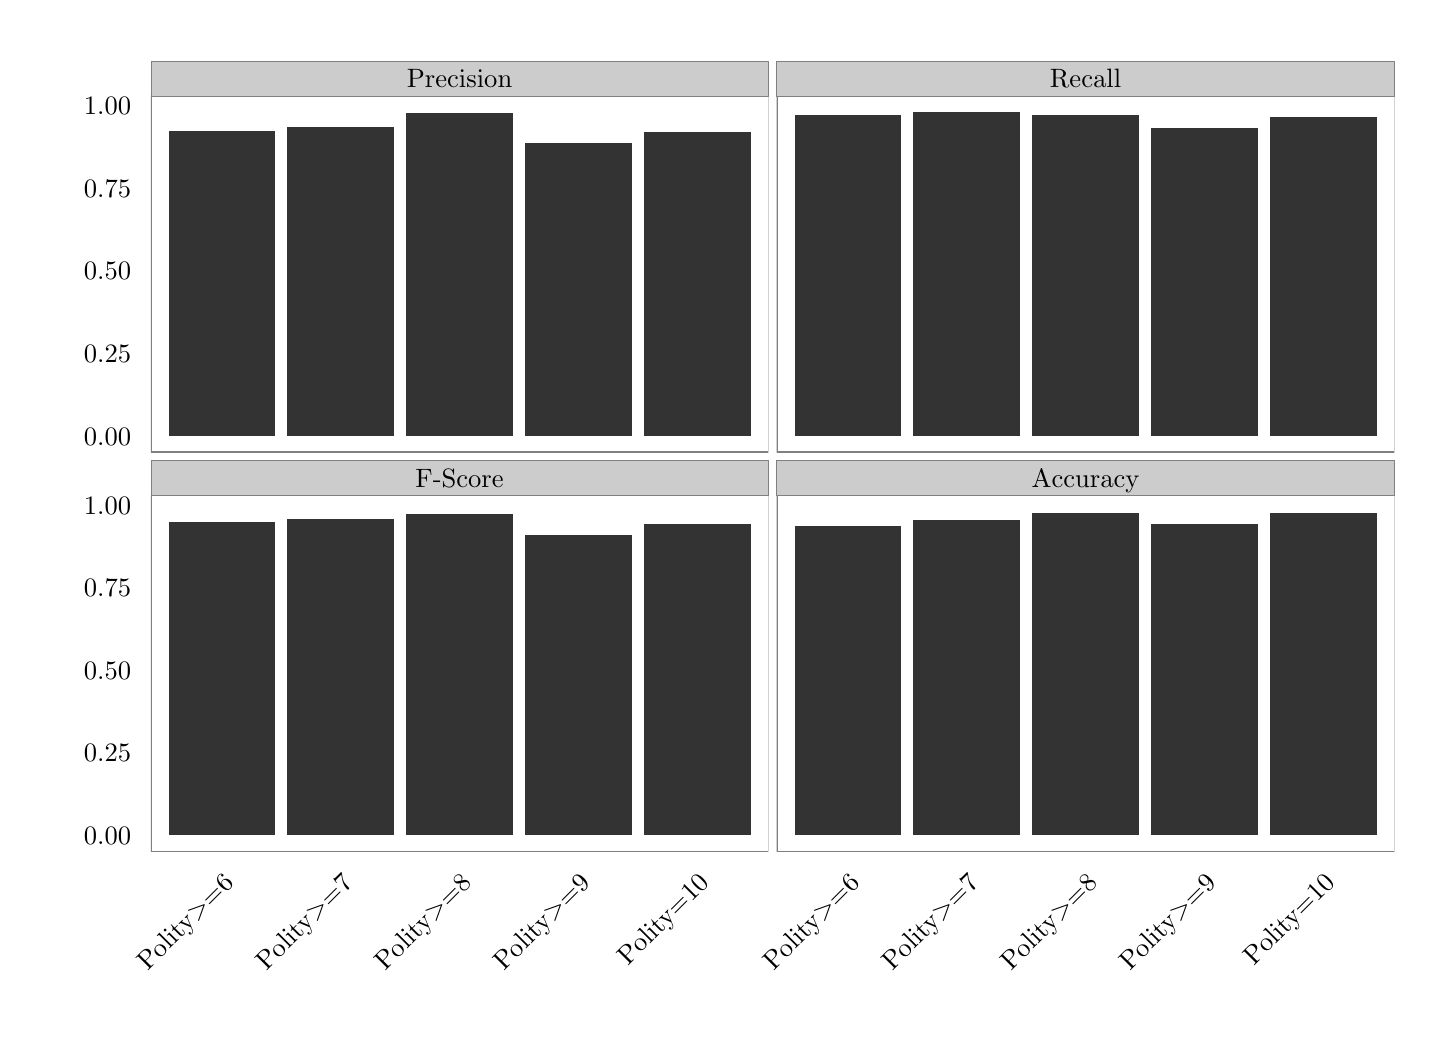
\begin{tikzpicture}[x=1pt,y=1pt]
\definecolor[named]{drawColor}{rgb}{0.00,0.00,0.00}
\definecolor[named]{fillColor}{rgb}{1.00,1.00,1.00}
\fill[color=fillColor,fill opacity=0.00,] (0,0) rectangle (505.89,361.35);
\begin{scope}
\path[clip] (  0.00,  0.00) rectangle (505.89,361.35);
\end{scope}
\begin{scope}
\path[clip] (  0.00,  0.00) rectangle (505.89,361.35);
\end{scope}
\begin{scope}
\path[clip] (  0.00,  0.00) rectangle (505.89,361.35);
\definecolor[named]{drawColor}{rgb}{1.00,1.00,1.00}
\definecolor[named]{fillColor}{rgb}{1.00,1.00,1.00}

\draw[color=drawColor,line width= 0.6pt,line cap=round,line join=round,fill=fillColor,] (  0.00,  0.00) rectangle (505.89,361.35);
\end{scope}
\begin{scope}
\path[clip] (  0.00,  0.00) rectangle (505.89,361.35);
\end{scope}
\begin{scope}
\path[clip] ( 44.49,208.00) rectangle (267.66,336.67);
\definecolor[named]{fillColor}{rgb}{1.00,1.00,1.00}

\draw[fill=fillColor,draw opacity=0.00,] ( 44.49,208.00) rectangle (267.66,336.67);
\definecolor[named]{fillColor}{rgb}{0.20,0.20,0.20}

\draw[fill=fillColor,draw opacity=0.00,] ( 50.92,213.85) rectangle ( 89.55,324.02);

\draw[fill=fillColor,draw opacity=0.00,] ( 93.84,213.85) rectangle (132.47,325.52);

\draw[fill=fillColor,draw opacity=0.00,] (136.76,213.85) rectangle (175.39,330.43);

\draw[fill=fillColor,draw opacity=0.00,] (179.68,213.85) rectangle (218.30,319.67);

\draw[fill=fillColor,draw opacity=0.00,] (222.60,213.85) rectangle (261.22,323.67);
\definecolor[named]{drawColor}{rgb}{0.50,0.50,0.50}

\draw[color=drawColor,line width= 0.6pt,line cap=round,line join=round,fill opacity=0.00,] ( 44.49,208.00) rectangle (267.66,336.67);
\end{scope}
\begin{scope}
\path[clip] (  0.00,  0.00) rectangle (505.89,361.35);
\end{scope}
\begin{scope}
\path[clip] (270.67,208.00) rectangle (493.85,336.67);
\definecolor[named]{fillColor}{rgb}{1.00,1.00,1.00}

\draw[fill=fillColor,draw opacity=0.00,] (270.67,208.00) rectangle (493.85,336.67);
\definecolor[named]{fillColor}{rgb}{0.20,0.20,0.20}

\draw[fill=fillColor,draw opacity=0.00,] (277.11,213.85) rectangle (315.73,329.95);

\draw[fill=fillColor,draw opacity=0.00,] (320.03,213.85) rectangle (358.65,330.82);

\draw[fill=fillColor,draw opacity=0.00,] (362.94,213.85) rectangle (401.57,329.68);

\draw[fill=fillColor,draw opacity=0.00,] (405.86,213.85) rectangle (444.49,324.98);

\draw[fill=fillColor,draw opacity=0.00,] (448.78,213.85) rectangle (487.41,329.01);
\definecolor[named]{drawColor}{rgb}{0.50,0.50,0.50}

\draw[color=drawColor,line width= 0.6pt,line cap=round,line join=round,fill opacity=0.00,] (270.67,208.00) rectangle (493.85,336.67);
\end{scope}
\begin{scope}
\path[clip] (  0.00,  0.00) rectangle (505.89,361.35);
\end{scope}
\begin{scope}
\path[clip] ( 44.49, 63.68) rectangle (267.66,192.35);
\definecolor[named]{fillColor}{rgb}{1.00,1.00,1.00}

\draw[fill=fillColor,draw opacity=0.00,] ( 44.49, 63.68) rectangle (267.66,192.35);
\definecolor[named]{fillColor}{rgb}{0.20,0.20,0.20}

\draw[fill=fillColor,draw opacity=0.00,] ( 50.92, 69.53) rectangle ( 89.55,182.59);

\draw[fill=fillColor,draw opacity=0.00,] ( 93.84, 69.53) rectangle (132.47,183.79);

\draw[fill=fillColor,draw opacity=0.00,] (136.76, 69.53) rectangle (175.39,185.74);

\draw[fill=fillColor,draw opacity=0.00,] (179.68, 69.53) rectangle (218.30,177.94);

\draw[fill=fillColor,draw opacity=0.00,] (222.60, 69.53) rectangle (261.22,181.96);
\definecolor[named]{drawColor}{rgb}{0.50,0.50,0.50}

\draw[color=drawColor,line width= 0.6pt,line cap=round,line join=round,fill opacity=0.00,] ( 44.49, 63.68) rectangle (267.66,192.35);
\end{scope}
\begin{scope}
\path[clip] (  0.00,  0.00) rectangle (505.89,361.35);
\end{scope}
\begin{scope}
\path[clip] (270.67, 63.68) rectangle (493.85,192.35);
\definecolor[named]{fillColor}{rgb}{1.00,1.00,1.00}

\draw[fill=fillColor,draw opacity=0.00,] (270.67, 63.68) rectangle (493.85,192.35);
\definecolor[named]{fillColor}{rgb}{0.20,0.20,0.20}

\draw[fill=fillColor,draw opacity=0.00,] (277.11, 69.53) rectangle (315.73,181.41);

\draw[fill=fillColor,draw opacity=0.00,] (320.03, 69.53) rectangle (358.65,183.60);

\draw[fill=fillColor,draw opacity=0.00,] (362.94, 69.53) rectangle (401.57,186.14);

\draw[fill=fillColor,draw opacity=0.00,] (405.86, 69.53) rectangle (444.49,181.92);

\draw[fill=fillColor,draw opacity=0.00,] (448.78, 69.53) rectangle (487.41,185.97);
\definecolor[named]{drawColor}{rgb}{0.50,0.50,0.50}

\draw[color=drawColor,line width= 0.6pt,line cap=round,line join=round,fill opacity=0.00,] (270.67, 63.68) rectangle (493.85,192.35);
\end{scope}
\begin{scope}
\path[clip] (  0.00,  0.00) rectangle (505.89,361.35);
\end{scope}
\begin{scope}
\path[clip] (  0.00,  0.00) rectangle (505.89,361.35);
\definecolor[named]{drawColor}{rgb}{0.50,0.50,0.50}
\definecolor[named]{fillColor}{rgb}{0.80,0.80,0.80}

\draw[color=drawColor,line width= 0.2pt,line cap=round,line join=round,fill=fillColor,] ( 44.49,336.67) rectangle (267.66,349.31);
\definecolor[named]{drawColor}{rgb}{0.00,0.00,0.00}

\node[color=drawColor,anchor=base,inner sep=0pt, outer sep=0pt, scale=  0.96] at (156.07,339.68) {Precision};
\end{scope}
\begin{scope}
\path[clip] (  0.00,  0.00) rectangle (505.89,361.35);
\end{scope}
\begin{scope}
\path[clip] (  0.00,  0.00) rectangle (505.89,361.35);
\definecolor[named]{drawColor}{rgb}{0.50,0.50,0.50}
\definecolor[named]{fillColor}{rgb}{0.80,0.80,0.80}

\draw[color=drawColor,line width= 0.2pt,line cap=round,line join=round,fill=fillColor,] (270.67,336.67) rectangle (493.85,349.31);
\definecolor[named]{drawColor}{rgb}{0.00,0.00,0.00}

\node[color=drawColor,anchor=base,inner sep=0pt, outer sep=0pt, scale=  0.96] at (382.26,339.68) {Recall};
\end{scope}
\begin{scope}
\path[clip] (  0.00,  0.00) rectangle (505.89,361.35);
\end{scope}
\begin{scope}
\path[clip] (  0.00,  0.00) rectangle (505.89,361.35);
\definecolor[named]{drawColor}{rgb}{0.50,0.50,0.50}
\definecolor[named]{fillColor}{rgb}{0.80,0.80,0.80}

\draw[color=drawColor,line width= 0.2pt,line cap=round,line join=round,fill=fillColor,] ( 44.49,192.35) rectangle (267.66,204.99);
\definecolor[named]{drawColor}{rgb}{0.00,0.00,0.00}

\node[color=drawColor,anchor=base,inner sep=0pt, outer sep=0pt, scale=  0.96] at (156.07,195.36) {F-Score};
\end{scope}
\begin{scope}
\path[clip] (  0.00,  0.00) rectangle (505.89,361.35);
\end{scope}
\begin{scope}
\path[clip] (  0.00,  0.00) rectangle (505.89,361.35);
\definecolor[named]{drawColor}{rgb}{0.50,0.50,0.50}
\definecolor[named]{fillColor}{rgb}{0.80,0.80,0.80}

\draw[color=drawColor,line width= 0.2pt,line cap=round,line join=round,fill=fillColor,] (270.67,192.35) rectangle (493.85,204.99);
\definecolor[named]{drawColor}{rgb}{0.00,0.00,0.00}

\node[color=drawColor,anchor=base,inner sep=0pt, outer sep=0pt, scale=  0.96] at (382.26,195.36) {Accuracy};
\end{scope}
\begin{scope}
\path[clip] (  0.00,  0.00) rectangle (505.89,361.35);
\end{scope}
\begin{scope}
\path[clip] (  0.00,  0.00) rectangle (505.89,361.35);
\end{scope}
\begin{scope}
\path[clip] (  0.00,  0.00) rectangle (505.89,361.35);
\definecolor[named]{drawColor}{rgb}{0.00,0.00,0.00}

\node[color=drawColor,anchor=base east,inner sep=0pt, outer sep=0pt, scale=  0.96] at ( 37.37,210.54) {0.00};

\node[color=drawColor,anchor=base east,inner sep=0pt, outer sep=0pt, scale=  0.96] at ( 37.37,240.37) {0.25};

\node[color=drawColor,anchor=base east,inner sep=0pt, outer sep=0pt, scale=  0.96] at ( 37.37,270.19) {0.50};

\node[color=drawColor,anchor=base east,inner sep=0pt, outer sep=0pt, scale=  0.96] at ( 37.37,300.02) {0.75};

\node[color=drawColor,anchor=base east,inner sep=0pt, outer sep=0pt, scale=  0.96] at ( 37.37,329.85) {1.00};
\end{scope}
\begin{scope}
\path[clip] (  0.00,  0.00) rectangle (505.89,361.35);
\end{scope}
\begin{scope}
\path[clip] (  0.00,  0.00) rectangle (505.89,361.35);
\end{scope}
\begin{scope}
\path[clip] (  0.00,  0.00) rectangle (505.89,361.35);
\end{scope}
\begin{scope}
\path[clip] (  0.00,  0.00) rectangle (505.89,361.35);
\end{scope}
\begin{scope}
\path[clip] (  0.00,  0.00) rectangle (505.89,361.35);
\end{scope}
\begin{scope}
\path[clip] (  0.00,  0.00) rectangle (505.89,361.35);
\end{scope}
\begin{scope}
\path[clip] (  0.00,  0.00) rectangle (505.89,361.35);
\end{scope}
\begin{scope}
\path[clip] (  0.00,  0.00) rectangle (505.89,361.35);
\end{scope}
\begin{scope}
\path[clip] (  0.00,  0.00) rectangle (505.89,361.35);
\end{scope}
\begin{scope}
\path[clip] (  0.00,  0.00) rectangle (505.89,361.35);
\definecolor[named]{drawColor}{rgb}{0.00,0.00,0.00}

\node[color=drawColor,anchor=base east,inner sep=0pt, outer sep=0pt, scale=  0.96] at ( 37.37, 66.22) {0.00};

\node[color=drawColor,anchor=base east,inner sep=0pt, outer sep=0pt, scale=  0.96] at ( 37.37, 96.05) {0.25};

\node[color=drawColor,anchor=base east,inner sep=0pt, outer sep=0pt, scale=  0.96] at ( 37.37,125.87) {0.50};

\node[color=drawColor,anchor=base east,inner sep=0pt, outer sep=0pt, scale=  0.96] at ( 37.37,155.70) {0.75};

\node[color=drawColor,anchor=base east,inner sep=0pt, outer sep=0pt, scale=  0.96] at ( 37.37,185.53) {1.00};
\end{scope}
\begin{scope}
\path[clip] (  0.00,  0.00) rectangle (505.89,361.35);
\end{scope}
\begin{scope}
\path[clip] (  0.00,  0.00) rectangle (505.89,361.35);
\end{scope}
\begin{scope}
\path[clip] (  0.00,  0.00) rectangle (505.89,361.35);
\end{scope}
\begin{scope}
\path[clip] (  0.00,  0.00) rectangle (505.89,361.35);
\end{scope}
\begin{scope}
\path[clip] (  0.00,  0.00) rectangle (505.89,361.35);
\end{scope}
\begin{scope}
\path[clip] (  0.00,  0.00) rectangle (505.89,361.35);
\end{scope}
\begin{scope}
\path[clip] (  0.00,  0.00) rectangle (505.89,361.35);
\end{scope}
\begin{scope}
\path[clip] (  0.00,  0.00) rectangle (505.89,361.35);
\end{scope}
\begin{scope}
\path[clip] (  0.00,  0.00) rectangle (505.89,361.35);
\end{scope}
\begin{scope}
\path[clip] (  0.00,  0.00) rectangle (505.89,361.35);
\end{scope}
\begin{scope}
\path[clip] (  0.00,  0.00) rectangle (505.89,361.35);
\end{scope}
\begin{scope}
\path[clip] (  0.00,  0.00) rectangle (505.89,361.35);
\end{scope}
\begin{scope}
\path[clip] (  0.00,  0.00) rectangle (505.89,361.35);
\end{scope}
\begin{scope}
\path[clip] (  0.00,  0.00) rectangle (505.89,361.35);
\end{scope}
\begin{scope}
\path[clip] (  0.00,  0.00) rectangle (505.89,361.35);
\end{scope}
\begin{scope}
\path[clip] (  0.00,  0.00) rectangle (505.89,361.35);
\definecolor[named]{drawColor}{rgb}{0.00,0.00,0.00}

\node[rotate= 45.00,color=drawColor,anchor=base east,inner sep=0pt, outer sep=0pt, scale=  0.96] at ( 74.91, 51.89) {Polity$>=$6};

\node[rotate= 45.00,color=drawColor,anchor=base east,inner sep=0pt, outer sep=0pt, scale=  0.96] at (117.83, 51.89) {Polity$>=$7};

\node[rotate= 45.00,color=drawColor,anchor=base east,inner sep=0pt, outer sep=0pt, scale=  0.96] at (160.75, 51.89) {Polity$>=$8};

\node[rotate= 45.00,color=drawColor,anchor=base east,inner sep=0pt, outer sep=0pt, scale=  0.96] at (203.67, 51.89) {Polity$>=$9};

\node[rotate= 45.00,color=drawColor,anchor=base east,inner sep=0pt, outer sep=0pt, scale=  0.96] at (246.58, 51.89) {Polity$=$10};
\end{scope}
\begin{scope}
\path[clip] (  0.00,  0.00) rectangle (505.89,361.35);
\end{scope}
\begin{scope}
\path[clip] (  0.00,  0.00) rectangle (505.89,361.35);
\end{scope}
\begin{scope}
\path[clip] (  0.00,  0.00) rectangle (505.89,361.35);
\end{scope}
\begin{scope}
\path[clip] (  0.00,  0.00) rectangle (505.89,361.35);
\end{scope}
\begin{scope}
\path[clip] (  0.00,  0.00) rectangle (505.89,361.35);
\end{scope}
\begin{scope}
\path[clip] (  0.00,  0.00) rectangle (505.89,361.35);
\end{scope}
\begin{scope}
\path[clip] (  0.00,  0.00) rectangle (505.89,361.35);
\end{scope}
\begin{scope}
\path[clip] (  0.00,  0.00) rectangle (505.89,361.35);
\definecolor[named]{drawColor}{rgb}{0.00,0.00,0.00}

\node[rotate= 45.00,color=drawColor,anchor=base east,inner sep=0pt, outer sep=0pt, scale=  0.96] at (301.10, 51.89) {Polity$>=$6};

\node[rotate= 45.00,color=drawColor,anchor=base east,inner sep=0pt, outer sep=0pt, scale=  0.96] at (344.02, 51.89) {Polity$>=$7};

\node[rotate= 45.00,color=drawColor,anchor=base east,inner sep=0pt, outer sep=0pt, scale=  0.96] at (386.93, 51.89) {Polity$>=$8};

\node[rotate= 45.00,color=drawColor,anchor=base east,inner sep=0pt, outer sep=0pt, scale=  0.96] at (429.85, 51.89) {Polity$>=$9};

\node[rotate= 45.00,color=drawColor,anchor=base east,inner sep=0pt, outer sep=0pt, scale=  0.96] at (472.77, 51.89) {Polity$=$10};
\end{scope}
\begin{scope}
\path[clip] (  0.00,  0.00) rectangle (505.89,361.35);
\end{scope}
\begin{scope}
\path[clip] (  0.00,  0.00) rectangle (505.89,361.35);
\end{scope}
\begin{scope}
\path[clip] (  0.00,  0.00) rectangle (505.89,361.35);
\end{scope}
\begin{scope}
\path[clip] (  0.00,  0.00) rectangle (505.89,361.35);
\end{scope}
\begin{scope}
\path[clip] (  0.00,  0.00) rectangle (505.89,361.35);
\end{scope}
\begin{scope}
\path[clip] (  0.00,  0.00) rectangle (505.89,361.35);
\end{scope}
\begin{scope}
\path[clip] (  0.00,  0.00) rectangle (505.89,361.35);
\end{scope}
\begin{scope}
\path[clip] (  0.00,  0.00) rectangle (505.89,361.35);
\end{scope}
\begin{scope}
\path[clip] (  0.00,  0.00) rectangle (505.89,361.35);
\end{scope}
\begin{scope}
\path[clip] (  0.00,  0.00) rectangle (505.89,361.35);
\end{scope}
\begin{scope}
\path[clip] (  0.00,  0.00) rectangle (505.89,361.35);
\end{scope}
\end{tikzpicture}
}	
\end{figure}

\end{frame}
%%%%%%%%%%%%%%%%%%%%%%%%%%%%%%%%%%%%%%%%%

%%%%%%%%%%%%%%%%%%%%%%%%%%%%%%%%%%%%%%%%%
% Separation plots
\begin{frame}
\frametitle{Out-of-Sample Separation Plots}

\begin{figure}
	\centering
	\begin{tabular}{ll}
    \hspace{-7mm}	
    \subfloat[][Polity$\geq$7]{
		\resizebox{0.5\textwidth}{!}{% Created by tikzDevice version 0.7.0 on 2014-12-22 11:52:47
% !TEX encoding = UTF-8 Unicode
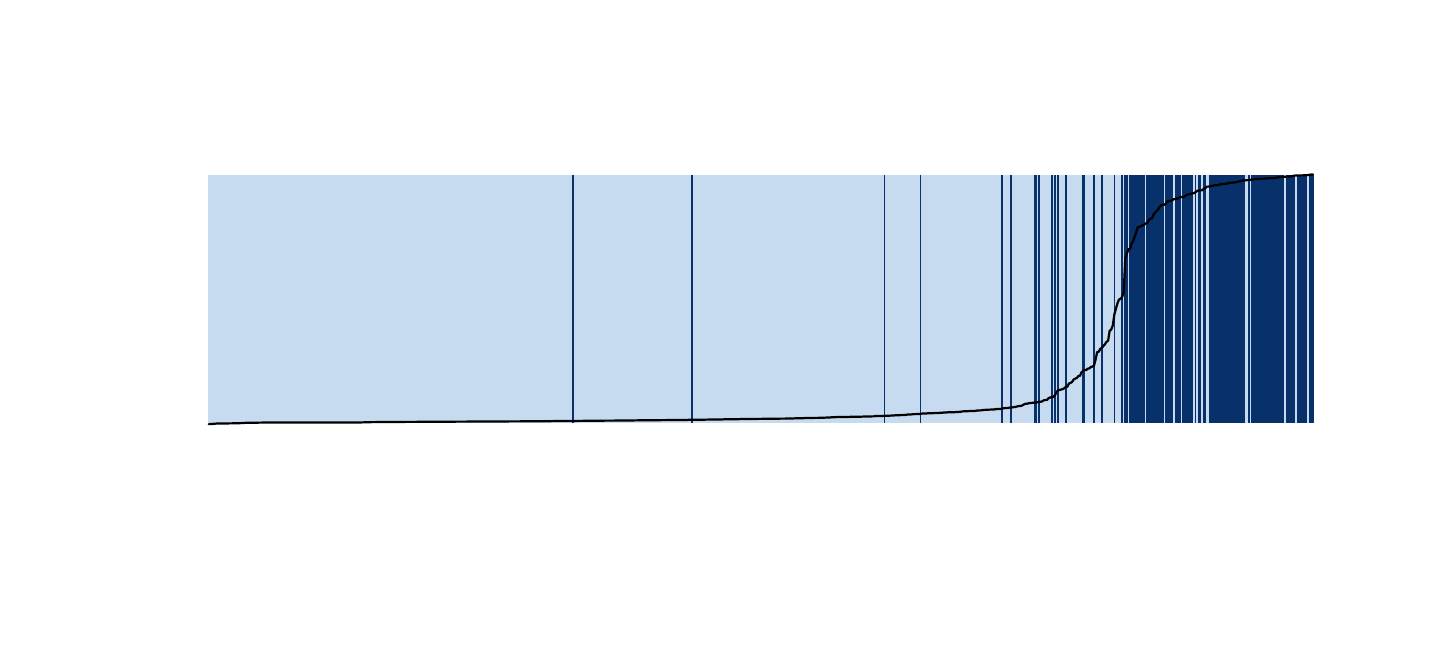
\begin{tikzpicture}[x=1pt,y=1pt]
\definecolor[named]{fillColor}{rgb}{1.00,1.00,1.00}
\path[use as bounding box,fill=fillColor,fill opacity=0.00] (0,0) rectangle (505.89,216.81);
\begin{scope}
\path[clip] ( 49.20, 61.20) rectangle (480.69,167.61);
\definecolor[named]{fillColor}{rgb}{0.78,0.86,0.94}

\path[fill=fillColor] ( 65.18, 74.10) rectangle ( 65.75,163.67);

\path[fill=fillColor] ( 65.75, 74.10) rectangle ( 66.31,163.67);

\path[fill=fillColor] ( 66.31, 74.10) rectangle ( 66.88,163.67);

\path[fill=fillColor] ( 66.88, 74.10) rectangle ( 67.44,163.67);

\path[fill=fillColor] ( 67.44, 74.10) rectangle ( 68.01,163.67);

\path[fill=fillColor] ( 68.01, 74.10) rectangle ( 68.57,163.67);

\path[fill=fillColor] ( 68.57, 74.10) rectangle ( 69.14,163.67);

\path[fill=fillColor] ( 69.14, 74.10) rectangle ( 69.70,163.67);

\path[fill=fillColor] ( 69.70, 74.10) rectangle ( 70.27,163.67);

\path[fill=fillColor] ( 70.27, 74.10) rectangle ( 70.83,163.67);

\path[fill=fillColor] ( 70.83, 74.10) rectangle ( 71.40,163.67);

\path[fill=fillColor] ( 71.40, 74.10) rectangle ( 71.96,163.67);

\path[fill=fillColor] ( 71.96, 74.10) rectangle ( 72.53,163.67);

\path[fill=fillColor] ( 72.53, 74.10) rectangle ( 73.09,163.67);

\path[fill=fillColor] ( 73.09, 74.10) rectangle ( 73.66,163.67);

\path[fill=fillColor] ( 73.66, 74.10) rectangle ( 74.22,163.67);

\path[fill=fillColor] ( 74.22, 74.10) rectangle ( 74.79,163.67);

\path[fill=fillColor] ( 74.79, 74.10) rectangle ( 75.35,163.67);

\path[fill=fillColor] ( 75.35, 74.10) rectangle ( 75.92,163.67);

\path[fill=fillColor] ( 75.92, 74.10) rectangle ( 76.48,163.67);

\path[fill=fillColor] ( 76.48, 74.10) rectangle ( 77.05,163.67);

\path[fill=fillColor] ( 77.05, 74.10) rectangle ( 77.61,163.67);

\path[fill=fillColor] ( 77.61, 74.10) rectangle ( 78.18,163.67);

\path[fill=fillColor] ( 78.18, 74.10) rectangle ( 78.74,163.67);

\path[fill=fillColor] ( 78.74, 74.10) rectangle ( 79.31,163.67);

\path[fill=fillColor] ( 79.31, 74.10) rectangle ( 79.87,163.67);

\path[fill=fillColor] ( 79.87, 74.10) rectangle ( 80.44,163.67);

\path[fill=fillColor] ( 80.44, 74.10) rectangle ( 81.00,163.67);

\path[fill=fillColor] ( 81.00, 74.10) rectangle ( 81.57,163.67);

\path[fill=fillColor] ( 81.57, 74.10) rectangle ( 82.13,163.67);

\path[fill=fillColor] ( 82.13, 74.10) rectangle ( 82.70,163.67);

\path[fill=fillColor] ( 82.70, 74.10) rectangle ( 83.26,163.67);

\path[fill=fillColor] ( 83.26, 74.10) rectangle ( 83.83,163.67);

\path[fill=fillColor] ( 83.83, 74.10) rectangle ( 84.39,163.67);

\path[fill=fillColor] ( 84.39, 74.10) rectangle ( 84.96,163.67);

\path[fill=fillColor] ( 84.96, 74.10) rectangle ( 85.52,163.67);

\path[fill=fillColor] ( 85.52, 74.10) rectangle ( 86.09,163.67);

\path[fill=fillColor] ( 86.09, 74.10) rectangle ( 86.66,163.67);

\path[fill=fillColor] ( 86.66, 74.10) rectangle ( 87.22,163.67);

\path[fill=fillColor] ( 87.22, 74.10) rectangle ( 87.79,163.67);

\path[fill=fillColor] ( 87.79, 74.10) rectangle ( 88.35,163.67);

\path[fill=fillColor] ( 88.35, 74.10) rectangle ( 88.92,163.67);

\path[fill=fillColor] ( 88.92, 74.10) rectangle ( 89.48,163.67);

\path[fill=fillColor] ( 89.48, 74.10) rectangle ( 90.05,163.67);

\path[fill=fillColor] ( 90.05, 74.10) rectangle ( 90.61,163.67);

\path[fill=fillColor] ( 90.61, 74.10) rectangle ( 91.18,163.67);

\path[fill=fillColor] ( 91.18, 74.10) rectangle ( 91.74,163.67);

\path[fill=fillColor] ( 91.74, 74.10) rectangle ( 92.31,163.67);

\path[fill=fillColor] ( 92.31, 74.10) rectangle ( 92.87,163.67);

\path[fill=fillColor] ( 92.87, 74.10) rectangle ( 93.44,163.67);

\path[fill=fillColor] ( 93.44, 74.10) rectangle ( 94.00,163.67);

\path[fill=fillColor] ( 94.00, 74.10) rectangle ( 94.57,163.67);

\path[fill=fillColor] ( 94.57, 74.10) rectangle ( 95.13,163.67);

\path[fill=fillColor] ( 95.13, 74.10) rectangle ( 95.70,163.67);

\path[fill=fillColor] ( 95.70, 74.10) rectangle ( 96.26,163.67);

\path[fill=fillColor] ( 96.26, 74.10) rectangle ( 96.83,163.67);

\path[fill=fillColor] ( 96.83, 74.10) rectangle ( 97.39,163.67);

\path[fill=fillColor] ( 97.39, 74.10) rectangle ( 97.96,163.67);

\path[fill=fillColor] ( 97.96, 74.10) rectangle ( 98.52,163.67);

\path[fill=fillColor] ( 98.52, 74.10) rectangle ( 99.09,163.67);

\path[fill=fillColor] ( 99.09, 74.10) rectangle ( 99.65,163.67);

\path[fill=fillColor] ( 99.65, 74.10) rectangle (100.22,163.67);

\path[fill=fillColor] (100.22, 74.10) rectangle (100.78,163.67);

\path[fill=fillColor] (100.78, 74.10) rectangle (101.35,163.67);

\path[fill=fillColor] (101.35, 74.10) rectangle (101.91,163.67);

\path[fill=fillColor] (101.91, 74.10) rectangle (102.48,163.67);

\path[fill=fillColor] (102.48, 74.10) rectangle (103.04,163.67);

\path[fill=fillColor] (103.04, 74.10) rectangle (103.61,163.67);

\path[fill=fillColor] (103.61, 74.10) rectangle (104.17,163.67);

\path[fill=fillColor] (104.17, 74.10) rectangle (104.74,163.67);

\path[fill=fillColor] (104.74, 74.10) rectangle (105.30,163.67);

\path[fill=fillColor] (105.30, 74.10) rectangle (105.87,163.67);

\path[fill=fillColor] (105.87, 74.10) rectangle (106.43,163.67);

\path[fill=fillColor] (106.43, 74.10) rectangle (107.00,163.67);

\path[fill=fillColor] (107.00, 74.10) rectangle (107.56,163.67);

\path[fill=fillColor] (107.56, 74.10) rectangle (108.13,163.67);

\path[fill=fillColor] (108.13, 74.10) rectangle (108.69,163.67);

\path[fill=fillColor] (108.69, 74.10) rectangle (109.26,163.67);

\path[fill=fillColor] (109.26, 74.10) rectangle (109.82,163.67);

\path[fill=fillColor] (109.82, 74.10) rectangle (110.39,163.67);

\path[fill=fillColor] (110.39, 74.10) rectangle (110.95,163.67);

\path[fill=fillColor] (110.95, 74.10) rectangle (111.52,163.67);

\path[fill=fillColor] (111.52, 74.10) rectangle (112.08,163.67);

\path[fill=fillColor] (112.08, 74.10) rectangle (112.65,163.67);

\path[fill=fillColor] (112.65, 74.10) rectangle (113.21,163.67);

\path[fill=fillColor] (113.21, 74.10) rectangle (113.78,163.67);

\path[fill=fillColor] (113.78, 74.10) rectangle (114.35,163.67);

\path[fill=fillColor] (114.35, 74.10) rectangle (114.91,163.67);

\path[fill=fillColor] (114.91, 74.10) rectangle (115.48,163.67);

\path[fill=fillColor] (115.48, 74.10) rectangle (116.04,163.67);

\path[fill=fillColor] (116.04, 74.10) rectangle (116.61,163.67);

\path[fill=fillColor] (116.61, 74.10) rectangle (117.17,163.67);

\path[fill=fillColor] (117.17, 74.10) rectangle (117.74,163.67);

\path[fill=fillColor] (117.74, 74.10) rectangle (118.30,163.67);

\path[fill=fillColor] (118.30, 74.10) rectangle (118.87,163.67);

\path[fill=fillColor] (118.87, 74.10) rectangle (119.43,163.67);

\path[fill=fillColor] (119.43, 74.10) rectangle (120.00,163.67);

\path[fill=fillColor] (120.00, 74.10) rectangle (120.56,163.67);

\path[fill=fillColor] (120.56, 74.10) rectangle (121.13,163.67);

\path[fill=fillColor] (121.13, 74.10) rectangle (121.69,163.67);

\path[fill=fillColor] (121.69, 74.10) rectangle (122.26,163.67);

\path[fill=fillColor] (122.26, 74.10) rectangle (122.82,163.67);

\path[fill=fillColor] (122.82, 74.10) rectangle (123.39,163.67);

\path[fill=fillColor] (123.39, 74.10) rectangle (123.95,163.67);

\path[fill=fillColor] (123.95, 74.10) rectangle (124.52,163.67);

\path[fill=fillColor] (124.52, 74.10) rectangle (125.08,163.67);

\path[fill=fillColor] (125.08, 74.10) rectangle (125.65,163.67);

\path[fill=fillColor] (125.65, 74.10) rectangle (126.21,163.67);

\path[fill=fillColor] (126.21, 74.10) rectangle (126.78,163.67);

\path[fill=fillColor] (126.78, 74.10) rectangle (127.34,163.67);

\path[fill=fillColor] (127.34, 74.10) rectangle (127.91,163.67);

\path[fill=fillColor] (127.91, 74.10) rectangle (128.47,163.67);

\path[fill=fillColor] (128.47, 74.10) rectangle (129.04,163.67);

\path[fill=fillColor] (129.04, 74.10) rectangle (129.60,163.67);

\path[fill=fillColor] (129.60, 74.10) rectangle (130.17,163.67);

\path[fill=fillColor] (130.17, 74.10) rectangle (130.73,163.67);

\path[fill=fillColor] (130.73, 74.10) rectangle (131.30,163.67);

\path[fill=fillColor] (131.30, 74.10) rectangle (131.86,163.67);

\path[fill=fillColor] (131.86, 74.10) rectangle (132.43,163.67);

\path[fill=fillColor] (132.43, 74.10) rectangle (132.99,163.67);

\path[fill=fillColor] (132.99, 74.10) rectangle (133.56,163.67);

\path[fill=fillColor] (133.56, 74.10) rectangle (134.12,163.67);

\path[fill=fillColor] (134.12, 74.10) rectangle (134.69,163.67);

\path[fill=fillColor] (134.69, 74.10) rectangle (135.25,163.67);

\path[fill=fillColor] (135.25, 74.10) rectangle (135.82,163.67);

\path[fill=fillColor] (135.82, 74.10) rectangle (136.38,163.67);

\path[fill=fillColor] (136.38, 74.10) rectangle (136.95,163.67);

\path[fill=fillColor] (136.95, 74.10) rectangle (137.51,163.67);

\path[fill=fillColor] (137.51, 74.10) rectangle (138.08,163.67);

\path[fill=fillColor] (138.08, 74.10) rectangle (138.64,163.67);

\path[fill=fillColor] (138.64, 74.10) rectangle (139.21,163.67);

\path[fill=fillColor] (139.21, 74.10) rectangle (139.77,163.67);

\path[fill=fillColor] (139.77, 74.10) rectangle (140.34,163.67);

\path[fill=fillColor] (140.34, 74.10) rectangle (140.90,163.67);

\path[fill=fillColor] (140.90, 74.10) rectangle (141.47,163.67);

\path[fill=fillColor] (141.47, 74.10) rectangle (142.04,163.67);

\path[fill=fillColor] (142.04, 74.10) rectangle (142.60,163.67);

\path[fill=fillColor] (142.60, 74.10) rectangle (143.17,163.67);

\path[fill=fillColor] (143.17, 74.10) rectangle (143.73,163.67);

\path[fill=fillColor] (143.73, 74.10) rectangle (144.30,163.67);

\path[fill=fillColor] (144.30, 74.10) rectangle (144.86,163.67);

\path[fill=fillColor] (144.86, 74.10) rectangle (145.43,163.67);

\path[fill=fillColor] (145.43, 74.10) rectangle (145.99,163.67);

\path[fill=fillColor] (145.99, 74.10) rectangle (146.56,163.67);

\path[fill=fillColor] (146.56, 74.10) rectangle (147.12,163.67);

\path[fill=fillColor] (147.12, 74.10) rectangle (147.69,163.67);

\path[fill=fillColor] (147.69, 74.10) rectangle (148.25,163.67);

\path[fill=fillColor] (148.25, 74.10) rectangle (148.82,163.67);

\path[fill=fillColor] (148.82, 74.10) rectangle (149.38,163.67);

\path[fill=fillColor] (149.38, 74.10) rectangle (149.95,163.67);

\path[fill=fillColor] (149.95, 74.10) rectangle (150.51,163.67);

\path[fill=fillColor] (150.51, 74.10) rectangle (151.08,163.67);

\path[fill=fillColor] (151.08, 74.10) rectangle (151.64,163.67);

\path[fill=fillColor] (151.64, 74.10) rectangle (152.21,163.67);

\path[fill=fillColor] (152.21, 74.10) rectangle (152.77,163.67);

\path[fill=fillColor] (152.77, 74.10) rectangle (153.34,163.67);

\path[fill=fillColor] (153.34, 74.10) rectangle (153.90,163.67);

\path[fill=fillColor] (153.90, 74.10) rectangle (154.47,163.67);

\path[fill=fillColor] (154.47, 74.10) rectangle (155.03,163.67);

\path[fill=fillColor] (155.03, 74.10) rectangle (155.60,163.67);

\path[fill=fillColor] (155.60, 74.10) rectangle (156.16,163.67);

\path[fill=fillColor] (156.16, 74.10) rectangle (156.73,163.67);

\path[fill=fillColor] (156.73, 74.10) rectangle (157.29,163.67);

\path[fill=fillColor] (157.29, 74.10) rectangle (157.86,163.67);

\path[fill=fillColor] (157.86, 74.10) rectangle (158.42,163.67);

\path[fill=fillColor] (158.42, 74.10) rectangle (158.99,163.67);

\path[fill=fillColor] (158.99, 74.10) rectangle (159.55,163.67);

\path[fill=fillColor] (159.55, 74.10) rectangle (160.12,163.67);

\path[fill=fillColor] (160.12, 74.10) rectangle (160.68,163.67);

\path[fill=fillColor] (160.68, 74.10) rectangle (161.25,163.67);

\path[fill=fillColor] (161.25, 74.10) rectangle (161.81,163.67);

\path[fill=fillColor] (161.81, 74.10) rectangle (162.38,163.67);

\path[fill=fillColor] (162.38, 74.10) rectangle (162.94,163.67);

\path[fill=fillColor] (162.94, 74.10) rectangle (163.51,163.67);

\path[fill=fillColor] (163.51, 74.10) rectangle (164.07,163.67);

\path[fill=fillColor] (164.07, 74.10) rectangle (164.64,163.67);

\path[fill=fillColor] (164.64, 74.10) rectangle (165.20,163.67);

\path[fill=fillColor] (165.20, 74.10) rectangle (165.77,163.67);

\path[fill=fillColor] (165.77, 74.10) rectangle (166.33,163.67);

\path[fill=fillColor] (166.33, 74.10) rectangle (166.90,163.67);

\path[fill=fillColor] (166.90, 74.10) rectangle (167.46,163.67);

\path[fill=fillColor] (167.46, 74.10) rectangle (168.03,163.67);

\path[fill=fillColor] (168.03, 74.10) rectangle (168.59,163.67);

\path[fill=fillColor] (168.59, 74.10) rectangle (169.16,163.67);

\path[fill=fillColor] (169.16, 74.10) rectangle (169.73,163.67);

\path[fill=fillColor] (169.73, 74.10) rectangle (170.29,163.67);

\path[fill=fillColor] (170.29, 74.10) rectangle (170.86,163.67);

\path[fill=fillColor] (170.86, 74.10) rectangle (171.42,163.67);

\path[fill=fillColor] (171.42, 74.10) rectangle (171.99,163.67);

\path[fill=fillColor] (171.99, 74.10) rectangle (172.55,163.67);

\path[fill=fillColor] (172.55, 74.10) rectangle (173.12,163.67);

\path[fill=fillColor] (173.12, 74.10) rectangle (173.68,163.67);

\path[fill=fillColor] (173.68, 74.10) rectangle (174.25,163.67);

\path[fill=fillColor] (174.25, 74.10) rectangle (174.81,163.67);

\path[fill=fillColor] (174.81, 74.10) rectangle (175.38,163.67);

\path[fill=fillColor] (175.38, 74.10) rectangle (175.94,163.67);

\path[fill=fillColor] (175.94, 74.10) rectangle (176.51,163.67);

\path[fill=fillColor] (176.51, 74.10) rectangle (177.07,163.67);

\path[fill=fillColor] (177.07, 74.10) rectangle (177.64,163.67);

\path[fill=fillColor] (177.64, 74.10) rectangle (178.20,163.67);

\path[fill=fillColor] (178.20, 74.10) rectangle (178.77,163.67);

\path[fill=fillColor] (178.77, 74.10) rectangle (179.33,163.67);

\path[fill=fillColor] (179.33, 74.10) rectangle (179.90,163.67);

\path[fill=fillColor] (179.90, 74.10) rectangle (180.46,163.67);

\path[fill=fillColor] (180.46, 74.10) rectangle (181.03,163.67);

\path[fill=fillColor] (181.03, 74.10) rectangle (181.59,163.67);

\path[fill=fillColor] (181.59, 74.10) rectangle (182.16,163.67);

\path[fill=fillColor] (182.16, 74.10) rectangle (182.72,163.67);

\path[fill=fillColor] (182.72, 74.10) rectangle (183.29,163.67);

\path[fill=fillColor] (183.29, 74.10) rectangle (183.85,163.67);

\path[fill=fillColor] (183.85, 74.10) rectangle (184.42,163.67);

\path[fill=fillColor] (184.42, 74.10) rectangle (184.98,163.67);

\path[fill=fillColor] (184.98, 74.10) rectangle (185.55,163.67);

\path[fill=fillColor] (185.55, 74.10) rectangle (186.11,163.67);

\path[fill=fillColor] (186.11, 74.10) rectangle (186.68,163.67);

\path[fill=fillColor] (186.68, 74.10) rectangle (187.24,163.67);

\path[fill=fillColor] (187.24, 74.10) rectangle (187.81,163.67);

\path[fill=fillColor] (187.81, 74.10) rectangle (188.37,163.67);

\path[fill=fillColor] (188.37, 74.10) rectangle (188.94,163.67);

\path[fill=fillColor] (188.94, 74.10) rectangle (189.50,163.67);

\path[fill=fillColor] (189.50, 74.10) rectangle (190.07,163.67);

\path[fill=fillColor] (190.07, 74.10) rectangle (190.63,163.67);

\path[fill=fillColor] (190.63, 74.10) rectangle (191.20,163.67);

\path[fill=fillColor] (191.20, 74.10) rectangle (191.76,163.67);

\path[fill=fillColor] (191.76, 74.10) rectangle (192.33,163.67);

\path[fill=fillColor] (192.33, 74.10) rectangle (192.89,163.67);

\path[fill=fillColor] (192.89, 74.10) rectangle (193.46,163.67);

\path[fill=fillColor] (193.46, 74.10) rectangle (194.02,163.67);

\path[fill=fillColor] (194.02, 74.10) rectangle (194.59,163.67);

\path[fill=fillColor] (194.59, 74.10) rectangle (195.15,163.67);

\path[fill=fillColor] (195.15, 74.10) rectangle (195.72,163.67);

\path[fill=fillColor] (195.72, 74.10) rectangle (196.28,163.67);

\path[fill=fillColor] (196.28, 74.10) rectangle (196.85,163.67);
\definecolor[named]{fillColor}{rgb}{0.03,0.19,0.42}

\path[fill=fillColor] (196.85, 74.10) rectangle (197.42,163.67);
\definecolor[named]{fillColor}{rgb}{0.78,0.86,0.94}

\path[fill=fillColor] (197.42, 74.10) rectangle (197.98,163.67);

\path[fill=fillColor] (197.98, 74.10) rectangle (198.55,163.67);

\path[fill=fillColor] (198.55, 74.10) rectangle (199.11,163.67);

\path[fill=fillColor] (199.11, 74.10) rectangle (199.68,163.67);

\path[fill=fillColor] (199.68, 74.10) rectangle (200.24,163.67);

\path[fill=fillColor] (200.24, 74.10) rectangle (200.81,163.67);

\path[fill=fillColor] (200.81, 74.10) rectangle (201.37,163.67);

\path[fill=fillColor] (201.37, 74.10) rectangle (201.94,163.67);

\path[fill=fillColor] (201.94, 74.10) rectangle (202.50,163.67);

\path[fill=fillColor] (202.50, 74.10) rectangle (203.07,163.67);

\path[fill=fillColor] (203.07, 74.10) rectangle (203.63,163.67);

\path[fill=fillColor] (203.63, 74.10) rectangle (204.20,163.67);

\path[fill=fillColor] (204.20, 74.10) rectangle (204.76,163.67);

\path[fill=fillColor] (204.76, 74.10) rectangle (205.33,163.67);

\path[fill=fillColor] (205.33, 74.10) rectangle (205.89,163.67);

\path[fill=fillColor] (205.89, 74.10) rectangle (206.46,163.67);

\path[fill=fillColor] (206.46, 74.10) rectangle (207.02,163.67);

\path[fill=fillColor] (207.02, 74.10) rectangle (207.59,163.67);

\path[fill=fillColor] (207.59, 74.10) rectangle (208.15,163.67);

\path[fill=fillColor] (208.15, 74.10) rectangle (208.72,163.67);

\path[fill=fillColor] (208.72, 74.10) rectangle (209.28,163.67);

\path[fill=fillColor] (209.28, 74.10) rectangle (209.85,163.67);

\path[fill=fillColor] (209.85, 74.10) rectangle (210.41,163.67);

\path[fill=fillColor] (210.41, 74.10) rectangle (210.98,163.67);

\path[fill=fillColor] (210.98, 74.10) rectangle (211.54,163.67);

\path[fill=fillColor] (211.54, 74.10) rectangle (212.11,163.67);

\path[fill=fillColor] (212.11, 74.10) rectangle (212.67,163.67);

\path[fill=fillColor] (212.67, 74.10) rectangle (213.24,163.67);

\path[fill=fillColor] (213.24, 74.10) rectangle (213.80,163.67);

\path[fill=fillColor] (213.80, 74.10) rectangle (214.37,163.67);

\path[fill=fillColor] (214.37, 74.10) rectangle (214.93,163.67);

\path[fill=fillColor] (214.93, 74.10) rectangle (215.50,163.67);

\path[fill=fillColor] (215.50, 74.10) rectangle (216.06,163.67);

\path[fill=fillColor] (216.06, 74.10) rectangle (216.63,163.67);

\path[fill=fillColor] (216.63, 74.10) rectangle (217.19,163.67);

\path[fill=fillColor] (217.19, 74.10) rectangle (217.76,163.67);

\path[fill=fillColor] (217.76, 74.10) rectangle (218.32,163.67);

\path[fill=fillColor] (218.32, 74.10) rectangle (218.89,163.67);

\path[fill=fillColor] (218.89, 74.10) rectangle (219.45,163.67);

\path[fill=fillColor] (219.45, 74.10) rectangle (220.02,163.67);

\path[fill=fillColor] (220.02, 74.10) rectangle (220.58,163.67);

\path[fill=fillColor] (220.58, 74.10) rectangle (221.15,163.67);

\path[fill=fillColor] (221.15, 74.10) rectangle (221.71,163.67);

\path[fill=fillColor] (221.71, 74.10) rectangle (222.28,163.67);

\path[fill=fillColor] (222.28, 74.10) rectangle (222.84,163.67);

\path[fill=fillColor] (222.84, 74.10) rectangle (223.41,163.67);

\path[fill=fillColor] (223.41, 74.10) rectangle (223.98,163.67);

\path[fill=fillColor] (223.98, 74.10) rectangle (224.54,163.67);

\path[fill=fillColor] (224.54, 74.10) rectangle (225.11,163.67);

\path[fill=fillColor] (225.11, 74.10) rectangle (225.67,163.67);

\path[fill=fillColor] (225.67, 74.10) rectangle (226.24,163.67);

\path[fill=fillColor] (226.24, 74.10) rectangle (226.80,163.67);

\path[fill=fillColor] (226.80, 74.10) rectangle (227.37,163.67);

\path[fill=fillColor] (227.37, 74.10) rectangle (227.93,163.67);

\path[fill=fillColor] (227.93, 74.10) rectangle (228.50,163.67);

\path[fill=fillColor] (228.50, 74.10) rectangle (229.06,163.67);

\path[fill=fillColor] (229.06, 74.10) rectangle (229.63,163.67);

\path[fill=fillColor] (229.63, 74.10) rectangle (230.19,163.67);

\path[fill=fillColor] (230.19, 74.10) rectangle (230.76,163.67);

\path[fill=fillColor] (230.76, 74.10) rectangle (231.32,163.67);

\path[fill=fillColor] (231.32, 74.10) rectangle (231.89,163.67);

\path[fill=fillColor] (231.89, 74.10) rectangle (232.45,163.67);

\path[fill=fillColor] (232.45, 74.10) rectangle (233.02,163.67);

\path[fill=fillColor] (233.02, 74.10) rectangle (233.58,163.67);

\path[fill=fillColor] (233.58, 74.10) rectangle (234.15,163.67);

\path[fill=fillColor] (234.15, 74.10) rectangle (234.71,163.67);

\path[fill=fillColor] (234.71, 74.10) rectangle (235.28,163.67);

\path[fill=fillColor] (235.28, 74.10) rectangle (235.84,163.67);

\path[fill=fillColor] (235.84, 74.10) rectangle (236.41,163.67);

\path[fill=fillColor] (236.41, 74.10) rectangle (236.97,163.67);

\path[fill=fillColor] (236.97, 74.10) rectangle (237.54,163.67);

\path[fill=fillColor] (237.54, 74.10) rectangle (238.10,163.67);

\path[fill=fillColor] (238.10, 74.10) rectangle (238.67,163.67);

\path[fill=fillColor] (238.67, 74.10) rectangle (239.23,163.67);

\path[fill=fillColor] (239.23, 74.10) rectangle (239.80,163.67);
\definecolor[named]{fillColor}{rgb}{0.03,0.19,0.42}

\path[fill=fillColor] (239.80, 74.10) rectangle (240.36,163.67);
\definecolor[named]{fillColor}{rgb}{0.78,0.86,0.94}

\path[fill=fillColor] (240.36, 74.10) rectangle (240.93,163.67);

\path[fill=fillColor] (240.93, 74.10) rectangle (241.49,163.67);

\path[fill=fillColor] (241.49, 74.10) rectangle (242.06,163.67);

\path[fill=fillColor] (242.06, 74.10) rectangle (242.62,163.67);

\path[fill=fillColor] (242.62, 74.10) rectangle (243.19,163.67);

\path[fill=fillColor] (243.19, 74.10) rectangle (243.75,163.67);

\path[fill=fillColor] (243.75, 74.10) rectangle (244.32,163.67);

\path[fill=fillColor] (244.32, 74.10) rectangle (244.88,163.67);

\path[fill=fillColor] (244.88, 74.10) rectangle (245.45,163.67);

\path[fill=fillColor] (245.45, 74.10) rectangle (246.01,163.67);

\path[fill=fillColor] (246.01, 74.10) rectangle (246.58,163.67);

\path[fill=fillColor] (246.58, 74.10) rectangle (247.14,163.67);

\path[fill=fillColor] (247.14, 74.10) rectangle (247.71,163.67);

\path[fill=fillColor] (247.71, 74.10) rectangle (248.27,163.67);

\path[fill=fillColor] (248.27, 74.10) rectangle (248.84,163.67);

\path[fill=fillColor] (248.84, 74.10) rectangle (249.40,163.67);

\path[fill=fillColor] (249.40, 74.10) rectangle (249.97,163.67);

\path[fill=fillColor] (249.97, 74.10) rectangle (250.53,163.67);

\path[fill=fillColor] (250.53, 74.10) rectangle (251.10,163.67);

\path[fill=fillColor] (251.10, 74.10) rectangle (251.67,163.67);

\path[fill=fillColor] (251.67, 74.10) rectangle (252.23,163.67);

\path[fill=fillColor] (252.23, 74.10) rectangle (252.80,163.67);

\path[fill=fillColor] (252.80, 74.10) rectangle (253.36,163.67);

\path[fill=fillColor] (253.36, 74.10) rectangle (253.93,163.67);

\path[fill=fillColor] (253.93, 74.10) rectangle (254.49,163.67);

\path[fill=fillColor] (254.49, 74.10) rectangle (255.06,163.67);

\path[fill=fillColor] (255.06, 74.10) rectangle (255.62,163.67);

\path[fill=fillColor] (255.62, 74.10) rectangle (256.19,163.67);

\path[fill=fillColor] (256.19, 74.10) rectangle (256.75,163.67);

\path[fill=fillColor] (256.75, 74.10) rectangle (257.32,163.67);

\path[fill=fillColor] (257.32, 74.10) rectangle (257.88,163.67);

\path[fill=fillColor] (257.88, 74.10) rectangle (258.45,163.67);

\path[fill=fillColor] (258.45, 74.10) rectangle (259.01,163.67);

\path[fill=fillColor] (259.01, 74.10) rectangle (259.58,163.67);

\path[fill=fillColor] (259.58, 74.10) rectangle (260.14,163.67);

\path[fill=fillColor] (260.14, 74.10) rectangle (260.71,163.67);

\path[fill=fillColor] (260.71, 74.10) rectangle (261.27,163.67);

\path[fill=fillColor] (261.27, 74.10) rectangle (261.84,163.67);

\path[fill=fillColor] (261.84, 74.10) rectangle (262.40,163.67);

\path[fill=fillColor] (262.40, 74.10) rectangle (262.97,163.67);

\path[fill=fillColor] (262.97, 74.10) rectangle (263.53,163.67);

\path[fill=fillColor] (263.53, 74.10) rectangle (264.10,163.67);

\path[fill=fillColor] (264.10, 74.10) rectangle (264.66,163.67);

\path[fill=fillColor] (264.66, 74.10) rectangle (265.23,163.67);

\path[fill=fillColor] (265.23, 74.10) rectangle (265.79,163.67);

\path[fill=fillColor] (265.79, 74.10) rectangle (266.36,163.67);

\path[fill=fillColor] (266.36, 74.10) rectangle (266.92,163.67);

\path[fill=fillColor] (266.92, 74.10) rectangle (267.49,163.67);

\path[fill=fillColor] (267.49, 74.10) rectangle (268.05,163.67);

\path[fill=fillColor] (268.05, 74.10) rectangle (268.62,163.67);

\path[fill=fillColor] (268.62, 74.10) rectangle (269.18,163.67);

\path[fill=fillColor] (269.18, 74.10) rectangle (269.75,163.67);

\path[fill=fillColor] (269.75, 74.10) rectangle (270.31,163.67);

\path[fill=fillColor] (270.31, 74.10) rectangle (270.88,163.67);

\path[fill=fillColor] (270.88, 74.10) rectangle (271.44,163.67);

\path[fill=fillColor] (271.44, 74.10) rectangle (272.01,163.67);

\path[fill=fillColor] (272.01, 74.10) rectangle (272.57,163.67);

\path[fill=fillColor] (272.57, 74.10) rectangle (273.14,163.67);

\path[fill=fillColor] (273.14, 74.10) rectangle (273.70,163.67);

\path[fill=fillColor] (273.70, 74.10) rectangle (274.27,163.67);

\path[fill=fillColor] (274.27, 74.10) rectangle (274.83,163.67);

\path[fill=fillColor] (274.83, 74.10) rectangle (275.40,163.67);

\path[fill=fillColor] (275.40, 74.10) rectangle (275.96,163.67);

\path[fill=fillColor] (275.96, 74.10) rectangle (276.53,163.67);

\path[fill=fillColor] (276.53, 74.10) rectangle (277.09,163.67);

\path[fill=fillColor] (277.09, 74.10) rectangle (277.66,163.67);

\path[fill=fillColor] (277.66, 74.10) rectangle (278.22,163.67);

\path[fill=fillColor] (278.22, 74.10) rectangle (278.79,163.67);

\path[fill=fillColor] (278.79, 74.10) rectangle (279.36,163.67);

\path[fill=fillColor] (279.36, 74.10) rectangle (279.92,163.67);

\path[fill=fillColor] (279.92, 74.10) rectangle (280.49,163.67);

\path[fill=fillColor] (280.49, 74.10) rectangle (281.05,163.67);

\path[fill=fillColor] (281.05, 74.10) rectangle (281.62,163.67);

\path[fill=fillColor] (281.62, 74.10) rectangle (282.18,163.67);

\path[fill=fillColor] (282.18, 74.10) rectangle (282.75,163.67);

\path[fill=fillColor] (282.75, 74.10) rectangle (283.31,163.67);

\path[fill=fillColor] (283.31, 74.10) rectangle (283.88,163.67);

\path[fill=fillColor] (283.88, 74.10) rectangle (284.44,163.67);

\path[fill=fillColor] (284.44, 74.10) rectangle (285.01,163.67);

\path[fill=fillColor] (285.01, 74.10) rectangle (285.57,163.67);

\path[fill=fillColor] (285.57, 74.10) rectangle (286.14,163.67);

\path[fill=fillColor] (286.14, 74.10) rectangle (286.70,163.67);

\path[fill=fillColor] (286.70, 74.10) rectangle (287.27,163.67);

\path[fill=fillColor] (287.27, 74.10) rectangle (287.83,163.67);

\path[fill=fillColor] (287.83, 74.10) rectangle (288.40,163.67);

\path[fill=fillColor] (288.40, 74.10) rectangle (288.96,163.67);

\path[fill=fillColor] (288.96, 74.10) rectangle (289.53,163.67);

\path[fill=fillColor] (289.53, 74.10) rectangle (290.09,163.67);

\path[fill=fillColor] (290.09, 74.10) rectangle (290.66,163.67);

\path[fill=fillColor] (290.66, 74.10) rectangle (291.22,163.67);

\path[fill=fillColor] (291.22, 74.10) rectangle (291.79,163.67);

\path[fill=fillColor] (291.79, 74.10) rectangle (292.35,163.67);

\path[fill=fillColor] (292.35, 74.10) rectangle (292.92,163.67);

\path[fill=fillColor] (292.92, 74.10) rectangle (293.48,163.67);

\path[fill=fillColor] (293.48, 74.10) rectangle (294.05,163.67);

\path[fill=fillColor] (294.05, 74.10) rectangle (294.61,163.67);

\path[fill=fillColor] (294.61, 74.10) rectangle (295.18,163.67);

\path[fill=fillColor] (295.18, 74.10) rectangle (295.74,163.67);

\path[fill=fillColor] (295.74, 74.10) rectangle (296.31,163.67);

\path[fill=fillColor] (296.31, 74.10) rectangle (296.87,163.67);

\path[fill=fillColor] (296.87, 74.10) rectangle (297.44,163.67);

\path[fill=fillColor] (297.44, 74.10) rectangle (298.00,163.67);

\path[fill=fillColor] (298.00, 74.10) rectangle (298.57,163.67);

\path[fill=fillColor] (298.57, 74.10) rectangle (299.13,163.67);

\path[fill=fillColor] (299.13, 74.10) rectangle (299.70,163.67);

\path[fill=fillColor] (299.70, 74.10) rectangle (300.26,163.67);

\path[fill=fillColor] (300.26, 74.10) rectangle (300.83,163.67);

\path[fill=fillColor] (300.83, 74.10) rectangle (301.39,163.67);

\path[fill=fillColor] (301.39, 74.10) rectangle (301.96,163.67);

\path[fill=fillColor] (301.96, 74.10) rectangle (302.52,163.67);

\path[fill=fillColor] (302.52, 74.10) rectangle (303.09,163.67);

\path[fill=fillColor] (303.09, 74.10) rectangle (303.65,163.67);

\path[fill=fillColor] (303.65, 74.10) rectangle (304.22,163.67);

\path[fill=fillColor] (304.22, 74.10) rectangle (304.78,163.67);

\path[fill=fillColor] (304.78, 74.10) rectangle (305.35,163.67);

\path[fill=fillColor] (305.35, 74.10) rectangle (305.91,163.67);

\path[fill=fillColor] (305.91, 74.10) rectangle (306.48,163.67);

\path[fill=fillColor] (306.48, 74.10) rectangle (307.05,163.67);

\path[fill=fillColor] (307.05, 74.10) rectangle (307.61,163.67);

\path[fill=fillColor] (307.61, 74.10) rectangle (308.18,163.67);

\path[fill=fillColor] (308.18, 74.10) rectangle (308.74,163.67);

\path[fill=fillColor] (308.74, 74.10) rectangle (309.31,163.67);
\definecolor[named]{fillColor}{rgb}{0.03,0.19,0.42}

\path[fill=fillColor] (309.31, 74.10) rectangle (309.87,163.67);
\definecolor[named]{fillColor}{rgb}{0.78,0.86,0.94}

\path[fill=fillColor] (309.87, 74.10) rectangle (310.44,163.67);

\path[fill=fillColor] (310.44, 74.10) rectangle (311.00,163.67);

\path[fill=fillColor] (311.00, 74.10) rectangle (311.57,163.67);

\path[fill=fillColor] (311.57, 74.10) rectangle (312.13,163.67);

\path[fill=fillColor] (312.13, 74.10) rectangle (312.70,163.67);

\path[fill=fillColor] (312.70, 74.10) rectangle (313.26,163.67);

\path[fill=fillColor] (313.26, 74.10) rectangle (313.83,163.67);

\path[fill=fillColor] (313.83, 74.10) rectangle (314.39,163.67);

\path[fill=fillColor] (314.39, 74.10) rectangle (314.96,163.67);

\path[fill=fillColor] (314.96, 74.10) rectangle (315.52,163.67);

\path[fill=fillColor] (315.52, 74.10) rectangle (316.09,163.67);

\path[fill=fillColor] (316.09, 74.10) rectangle (316.65,163.67);

\path[fill=fillColor] (316.65, 74.10) rectangle (317.22,163.67);

\path[fill=fillColor] (317.22, 74.10) rectangle (317.78,163.67);

\path[fill=fillColor] (317.78, 74.10) rectangle (318.35,163.67);

\path[fill=fillColor] (318.35, 74.10) rectangle (318.91,163.67);

\path[fill=fillColor] (318.91, 74.10) rectangle (319.48,163.67);

\path[fill=fillColor] (319.48, 74.10) rectangle (320.04,163.67);

\path[fill=fillColor] (320.04, 74.10) rectangle (320.61,163.67);

\path[fill=fillColor] (320.61, 74.10) rectangle (321.17,163.67);

\path[fill=fillColor] (321.17, 74.10) rectangle (321.74,163.67);

\path[fill=fillColor] (321.74, 74.10) rectangle (322.30,163.67);
\definecolor[named]{fillColor}{rgb}{0.03,0.19,0.42}

\path[fill=fillColor] (322.30, 74.10) rectangle (322.87,163.67);
\definecolor[named]{fillColor}{rgb}{0.78,0.86,0.94}

\path[fill=fillColor] (322.87, 74.10) rectangle (323.43,163.67);

\path[fill=fillColor] (323.43, 74.10) rectangle (324.00,163.67);

\path[fill=fillColor] (324.00, 74.10) rectangle (324.56,163.67);

\path[fill=fillColor] (324.56, 74.10) rectangle (325.13,163.67);

\path[fill=fillColor] (325.13, 74.10) rectangle (325.69,163.67);

\path[fill=fillColor] (325.69, 74.10) rectangle (326.26,163.67);

\path[fill=fillColor] (326.26, 74.10) rectangle (326.82,163.67);

\path[fill=fillColor] (326.82, 74.10) rectangle (327.39,163.67);

\path[fill=fillColor] (327.39, 74.10) rectangle (327.95,163.67);

\path[fill=fillColor] (327.95, 74.10) rectangle (328.52,163.67);

\path[fill=fillColor] (328.52, 74.10) rectangle (329.08,163.67);

\path[fill=fillColor] (329.08, 74.10) rectangle (329.65,163.67);

\path[fill=fillColor] (329.65, 74.10) rectangle (330.21,163.67);

\path[fill=fillColor] (330.21, 74.10) rectangle (330.78,163.67);

\path[fill=fillColor] (330.78, 74.10) rectangle (331.34,163.67);

\path[fill=fillColor] (331.34, 74.10) rectangle (331.91,163.67);

\path[fill=fillColor] (331.91, 74.10) rectangle (332.47,163.67);

\path[fill=fillColor] (332.47, 74.10) rectangle (333.04,163.67);

\path[fill=fillColor] (333.04, 74.10) rectangle (333.61,163.67);

\path[fill=fillColor] (333.61, 74.10) rectangle (334.17,163.67);

\path[fill=fillColor] (334.17, 74.10) rectangle (334.74,163.67);

\path[fill=fillColor] (334.74, 74.10) rectangle (335.30,163.67);

\path[fill=fillColor] (335.30, 74.10) rectangle (335.87,163.67);

\path[fill=fillColor] (335.87, 74.10) rectangle (336.43,163.67);

\path[fill=fillColor] (336.43, 74.10) rectangle (337.00,163.67);

\path[fill=fillColor] (337.00, 74.10) rectangle (337.56,163.67);

\path[fill=fillColor] (337.56, 74.10) rectangle (338.13,163.67);

\path[fill=fillColor] (338.13, 74.10) rectangle (338.69,163.67);

\path[fill=fillColor] (338.69, 74.10) rectangle (339.26,163.67);

\path[fill=fillColor] (339.26, 74.10) rectangle (339.82,163.67);

\path[fill=fillColor] (339.82, 74.10) rectangle (340.39,163.67);

\path[fill=fillColor] (340.39, 74.10) rectangle (340.95,163.67);

\path[fill=fillColor] (340.95, 74.10) rectangle (341.52,163.67);

\path[fill=fillColor] (341.52, 74.10) rectangle (342.08,163.67);

\path[fill=fillColor] (342.08, 74.10) rectangle (342.65,163.67);

\path[fill=fillColor] (342.65, 74.10) rectangle (343.21,163.67);

\path[fill=fillColor] (343.21, 74.10) rectangle (343.78,163.67);

\path[fill=fillColor] (343.78, 74.10) rectangle (344.34,163.67);

\path[fill=fillColor] (344.34, 74.10) rectangle (344.91,163.67);

\path[fill=fillColor] (344.91, 74.10) rectangle (345.47,163.67);

\path[fill=fillColor] (345.47, 74.10) rectangle (346.04,163.67);

\path[fill=fillColor] (346.04, 74.10) rectangle (346.60,163.67);

\path[fill=fillColor] (346.60, 74.10) rectangle (347.17,163.67);

\path[fill=fillColor] (347.17, 74.10) rectangle (347.73,163.67);

\path[fill=fillColor] (347.73, 74.10) rectangle (348.30,163.67);

\path[fill=fillColor] (348.30, 74.10) rectangle (348.86,163.67);

\path[fill=fillColor] (348.86, 74.10) rectangle (349.43,163.67);

\path[fill=fillColor] (349.43, 74.10) rectangle (349.99,163.67);

\path[fill=fillColor] (349.99, 74.10) rectangle (350.56,163.67);

\path[fill=fillColor] (350.56, 74.10) rectangle (351.12,163.67);

\path[fill=fillColor] (351.12, 74.10) rectangle (351.69,163.67);
\definecolor[named]{fillColor}{rgb}{0.03,0.19,0.42}

\path[fill=fillColor] (351.69, 74.10) rectangle (352.25,163.67);
\definecolor[named]{fillColor}{rgb}{0.78,0.86,0.94}

\path[fill=fillColor] (352.25, 74.10) rectangle (352.82,163.67);

\path[fill=fillColor] (352.82, 74.10) rectangle (353.38,163.67);

\path[fill=fillColor] (353.38, 74.10) rectangle (353.95,163.67);

\path[fill=fillColor] (353.95, 74.10) rectangle (354.51,163.67);

\path[fill=fillColor] (354.51, 74.10) rectangle (355.08,163.67);
\definecolor[named]{fillColor}{rgb}{0.03,0.19,0.42}

\path[fill=fillColor] (355.08, 74.10) rectangle (355.64,163.67);
\definecolor[named]{fillColor}{rgb}{0.78,0.86,0.94}

\path[fill=fillColor] (355.64, 74.10) rectangle (356.21,163.67);

\path[fill=fillColor] (356.21, 74.10) rectangle (356.77,163.67);

\path[fill=fillColor] (356.77, 74.10) rectangle (357.34,163.67);

\path[fill=fillColor] (357.34, 74.10) rectangle (357.90,163.67);

\path[fill=fillColor] (357.90, 74.10) rectangle (358.47,163.67);

\path[fill=fillColor] (358.47, 74.10) rectangle (359.03,163.67);

\path[fill=fillColor] (359.03, 74.10) rectangle (359.60,163.67);

\path[fill=fillColor] (359.60, 74.10) rectangle (360.16,163.67);

\path[fill=fillColor] (360.16, 74.10) rectangle (360.73,163.67);

\path[fill=fillColor] (360.73, 74.10) rectangle (361.30,163.67);

\path[fill=fillColor] (361.30, 74.10) rectangle (361.86,163.67);

\path[fill=fillColor] (361.86, 74.10) rectangle (362.43,163.67);

\path[fill=fillColor] (362.43, 74.10) rectangle (362.99,163.67);

\path[fill=fillColor] (362.99, 74.10) rectangle (363.56,163.67);
\definecolor[named]{fillColor}{rgb}{0.03,0.19,0.42}

\path[fill=fillColor] (363.56, 74.10) rectangle (364.12,163.67);

\path[fill=fillColor] (364.12, 74.10) rectangle (364.69,163.67);
\definecolor[named]{fillColor}{rgb}{0.78,0.86,0.94}

\path[fill=fillColor] (364.69, 74.10) rectangle (365.25,163.67);
\definecolor[named]{fillColor}{rgb}{0.03,0.19,0.42}

\path[fill=fillColor] (365.25, 74.10) rectangle (365.82,163.67);
\definecolor[named]{fillColor}{rgb}{0.78,0.86,0.94}

\path[fill=fillColor] (365.82, 74.10) rectangle (366.38,163.67);

\path[fill=fillColor] (366.38, 74.10) rectangle (366.95,163.67);

\path[fill=fillColor] (366.95, 74.10) rectangle (367.51,163.67);

\path[fill=fillColor] (367.51, 74.10) rectangle (368.08,163.67);

\path[fill=fillColor] (368.08, 74.10) rectangle (368.64,163.67);

\path[fill=fillColor] (368.64, 74.10) rectangle (369.21,163.67);

\path[fill=fillColor] (369.21, 74.10) rectangle (369.77,163.67);
\definecolor[named]{fillColor}{rgb}{0.03,0.19,0.42}

\path[fill=fillColor] (369.77, 74.10) rectangle (370.34,163.67);
\definecolor[named]{fillColor}{rgb}{0.78,0.86,0.94}

\path[fill=fillColor] (370.34, 74.10) rectangle (370.90,163.67);
\definecolor[named]{fillColor}{rgb}{0.03,0.19,0.42}

\path[fill=fillColor] (370.90, 74.10) rectangle (371.47,163.67);
\definecolor[named]{fillColor}{rgb}{0.78,0.86,0.94}

\path[fill=fillColor] (371.47, 74.10) rectangle (372.03,163.67);
\definecolor[named]{fillColor}{rgb}{0.03,0.19,0.42}

\path[fill=fillColor] (372.03, 74.10) rectangle (372.60,163.67);
\definecolor[named]{fillColor}{rgb}{0.78,0.86,0.94}

\path[fill=fillColor] (372.60, 74.10) rectangle (373.16,163.67);

\path[fill=fillColor] (373.16, 74.10) rectangle (373.73,163.67);

\path[fill=fillColor] (373.73, 74.10) rectangle (374.29,163.67);

\path[fill=fillColor] (374.29, 74.10) rectangle (374.86,163.67);
\definecolor[named]{fillColor}{rgb}{0.03,0.19,0.42}

\path[fill=fillColor] (374.86, 74.10) rectangle (375.42,163.67);
\definecolor[named]{fillColor}{rgb}{0.78,0.86,0.94}

\path[fill=fillColor] (375.42, 74.10) rectangle (375.99,163.67);

\path[fill=fillColor] (375.99, 74.10) rectangle (376.55,163.67);

\path[fill=fillColor] (376.55, 74.10) rectangle (377.12,163.67);

\path[fill=fillColor] (377.12, 74.10) rectangle (377.68,163.67);

\path[fill=fillColor] (377.68, 74.10) rectangle (378.25,163.67);

\path[fill=fillColor] (378.25, 74.10) rectangle (378.81,163.67);

\path[fill=fillColor] (378.81, 74.10) rectangle (379.38,163.67);

\path[fill=fillColor] (379.38, 74.10) rectangle (379.94,163.67);

\path[fill=fillColor] (379.94, 74.10) rectangle (380.51,163.67);

\path[fill=fillColor] (380.51, 74.10) rectangle (381.07,163.67);
\definecolor[named]{fillColor}{rgb}{0.03,0.19,0.42}

\path[fill=fillColor] (381.07, 74.10) rectangle (381.64,163.67);

\path[fill=fillColor] (381.64, 74.10) rectangle (382.20,163.67);
\definecolor[named]{fillColor}{rgb}{0.78,0.86,0.94}

\path[fill=fillColor] (382.20, 74.10) rectangle (382.77,163.67);

\path[fill=fillColor] (382.77, 74.10) rectangle (383.33,163.67);

\path[fill=fillColor] (383.33, 74.10) rectangle (383.90,163.67);

\path[fill=fillColor] (383.90, 74.10) rectangle (384.46,163.67);

\path[fill=fillColor] (384.46, 74.10) rectangle (385.03,163.67);
\definecolor[named]{fillColor}{rgb}{0.03,0.19,0.42}

\path[fill=fillColor] (385.03, 74.10) rectangle (385.59,163.67);
\definecolor[named]{fillColor}{rgb}{0.78,0.86,0.94}

\path[fill=fillColor] (385.59, 74.10) rectangle (386.16,163.67);

\path[fill=fillColor] (386.16, 74.10) rectangle (386.72,163.67);

\path[fill=fillColor] (386.72, 74.10) rectangle (387.29,163.67);

\path[fill=fillColor] (387.29, 74.10) rectangle (387.85,163.67);
\definecolor[named]{fillColor}{rgb}{0.03,0.19,0.42}

\path[fill=fillColor] (387.85, 74.10) rectangle (388.42,163.67);
\definecolor[named]{fillColor}{rgb}{0.78,0.86,0.94}

\path[fill=fillColor] (388.42, 74.10) rectangle (388.99,163.67);

\path[fill=fillColor] (388.99, 74.10) rectangle (389.55,163.67);

\path[fill=fillColor] (389.55, 74.10) rectangle (390.12,163.67);

\path[fill=fillColor] (390.12, 74.10) rectangle (390.68,163.67);

\path[fill=fillColor] (390.68, 74.10) rectangle (391.25,163.67);

\path[fill=fillColor] (391.25, 74.10) rectangle (391.81,163.67);

\path[fill=fillColor] (391.81, 74.10) rectangle (392.38,163.67);
\definecolor[named]{fillColor}{rgb}{0.03,0.19,0.42}

\path[fill=fillColor] (392.38, 74.10) rectangle (392.94,163.67);
\definecolor[named]{fillColor}{rgb}{0.78,0.86,0.94}

\path[fill=fillColor] (392.94, 74.10) rectangle (393.51,163.67);

\path[fill=fillColor] (393.51, 74.10) rectangle (394.07,163.67);

\path[fill=fillColor] (394.07, 74.10) rectangle (394.64,163.67);

\path[fill=fillColor] (394.64, 74.10) rectangle (395.20,163.67);
\definecolor[named]{fillColor}{rgb}{0.03,0.19,0.42}

\path[fill=fillColor] (395.20, 74.10) rectangle (395.77,163.67);
\definecolor[named]{fillColor}{rgb}{0.78,0.86,0.94}

\path[fill=fillColor] (395.77, 74.10) rectangle (396.33,163.67);
\definecolor[named]{fillColor}{rgb}{0.03,0.19,0.42}

\path[fill=fillColor] (396.33, 74.10) rectangle (396.90,163.67);

\path[fill=fillColor] (396.90, 74.10) rectangle (397.46,163.67);
\definecolor[named]{fillColor}{rgb}{0.78,0.86,0.94}

\path[fill=fillColor] (397.46, 74.10) rectangle (398.03,163.67);
\definecolor[named]{fillColor}{rgb}{0.03,0.19,0.42}

\path[fill=fillColor] (398.03, 74.10) rectangle (398.59,163.67);

\path[fill=fillColor] (398.59, 74.10) rectangle (399.16,163.67);

\path[fill=fillColor] (399.16, 74.10) rectangle (399.72,163.67);

\path[fill=fillColor] (399.72, 74.10) rectangle (400.29,163.67);

\path[fill=fillColor] (400.29, 74.10) rectangle (400.85,163.67);

\path[fill=fillColor] (400.85, 74.10) rectangle (401.42,163.67);

\path[fill=fillColor] (401.42, 74.10) rectangle (401.98,163.67);

\path[fill=fillColor] (401.98, 74.10) rectangle (402.55,163.67);

\path[fill=fillColor] (402.55, 74.10) rectangle (403.11,163.67);

\path[fill=fillColor] (403.11, 74.10) rectangle (403.68,163.67);
\definecolor[named]{fillColor}{rgb}{0.78,0.86,0.94}

\path[fill=fillColor] (403.68, 74.10) rectangle (404.24,163.67);
\definecolor[named]{fillColor}{rgb}{0.03,0.19,0.42}

\path[fill=fillColor] (404.24, 74.10) rectangle (404.81,163.67);

\path[fill=fillColor] (404.81, 74.10) rectangle (405.37,163.67);

\path[fill=fillColor] (405.37, 74.10) rectangle (405.94,163.67);

\path[fill=fillColor] (405.94, 74.10) rectangle (406.50,163.67);

\path[fill=fillColor] (406.50, 74.10) rectangle (407.07,163.67);

\path[fill=fillColor] (407.07, 74.10) rectangle (407.63,163.67);

\path[fill=fillColor] (407.63, 74.10) rectangle (408.20,163.67);

\path[fill=fillColor] (408.20, 74.10) rectangle (408.76,163.67);

\path[fill=fillColor] (408.76, 74.10) rectangle (409.33,163.67);

\path[fill=fillColor] (409.33, 74.10) rectangle (409.89,163.67);

\path[fill=fillColor] (409.89, 74.10) rectangle (410.46,163.67);
\definecolor[named]{fillColor}{rgb}{0.78,0.86,0.94}

\path[fill=fillColor] (410.46, 74.10) rectangle (411.02,163.67);
\definecolor[named]{fillColor}{rgb}{0.03,0.19,0.42}

\path[fill=fillColor] (411.02, 74.10) rectangle (411.59,163.67);

\path[fill=fillColor] (411.59, 74.10) rectangle (412.15,163.67);

\path[fill=fillColor] (412.15, 74.10) rectangle (412.72,163.67);

\path[fill=fillColor] (412.72, 74.10) rectangle (413.28,163.67);

\path[fill=fillColor] (413.28, 74.10) rectangle (413.85,163.67);
\definecolor[named]{fillColor}{rgb}{0.78,0.86,0.94}

\path[fill=fillColor] (413.85, 74.10) rectangle (414.41,163.67);
\definecolor[named]{fillColor}{rgb}{0.03,0.19,0.42}

\path[fill=fillColor] (414.41, 74.10) rectangle (414.98,163.67);

\path[fill=fillColor] (414.98, 74.10) rectangle (415.54,163.67);

\path[fill=fillColor] (415.54, 74.10) rectangle (416.11,163.67);

\path[fill=fillColor] (416.11, 74.10) rectangle (416.68,163.67);
\definecolor[named]{fillColor}{rgb}{0.78,0.86,0.94}

\path[fill=fillColor] (416.68, 74.10) rectangle (417.24,163.67);
\definecolor[named]{fillColor}{rgb}{0.03,0.19,0.42}

\path[fill=fillColor] (417.24, 74.10) rectangle (417.81,163.67);

\path[fill=fillColor] (417.81, 74.10) rectangle (418.37,163.67);

\path[fill=fillColor] (418.37, 74.10) rectangle (418.94,163.67);

\path[fill=fillColor] (418.94, 74.10) rectangle (419.50,163.67);

\path[fill=fillColor] (419.50, 74.10) rectangle (420.07,163.67);

\path[fill=fillColor] (420.07, 74.10) rectangle (420.63,163.67);

\path[fill=fillColor] (420.63, 74.10) rectangle (421.20,163.67);
\definecolor[named]{fillColor}{rgb}{0.78,0.86,0.94}

\path[fill=fillColor] (421.20, 74.10) rectangle (421.76,163.67);
\definecolor[named]{fillColor}{rgb}{0.03,0.19,0.42}

\path[fill=fillColor] (421.76, 74.10) rectangle (422.33,163.67);
\definecolor[named]{fillColor}{rgb}{0.78,0.86,0.94}

\path[fill=fillColor] (422.33, 74.10) rectangle (422.89,163.67);
\definecolor[named]{fillColor}{rgb}{0.03,0.19,0.42}

\path[fill=fillColor] (422.89, 74.10) rectangle (423.46,163.67);

\path[fill=fillColor] (423.46, 74.10) rectangle (424.02,163.67);
\definecolor[named]{fillColor}{rgb}{0.78,0.86,0.94}

\path[fill=fillColor] (424.02, 74.10) rectangle (424.59,163.67);
\definecolor[named]{fillColor}{rgb}{0.03,0.19,0.42}

\path[fill=fillColor] (424.59, 74.10) rectangle (425.15,163.67);

\path[fill=fillColor] (425.15, 74.10) rectangle (425.72,163.67);
\definecolor[named]{fillColor}{rgb}{0.78,0.86,0.94}

\path[fill=fillColor] (425.72, 74.10) rectangle (426.28,163.67);

\path[fill=fillColor] (426.28, 74.10) rectangle (426.85,163.67);
\definecolor[named]{fillColor}{rgb}{0.03,0.19,0.42}

\path[fill=fillColor] (426.85, 74.10) rectangle (427.41,163.67);

\path[fill=fillColor] (427.41, 74.10) rectangle (427.98,163.67);

\path[fill=fillColor] (427.98, 74.10) rectangle (428.54,163.67);

\path[fill=fillColor] (428.54, 74.10) rectangle (429.11,163.67);

\path[fill=fillColor] (429.11, 74.10) rectangle (429.67,163.67);

\path[fill=fillColor] (429.67, 74.10) rectangle (430.24,163.67);

\path[fill=fillColor] (430.24, 74.10) rectangle (430.80,163.67);

\path[fill=fillColor] (430.80, 74.10) rectangle (431.37,163.67);

\path[fill=fillColor] (431.37, 74.10) rectangle (431.93,163.67);

\path[fill=fillColor] (431.93, 74.10) rectangle (432.50,163.67);

\path[fill=fillColor] (432.50, 74.10) rectangle (433.06,163.67);

\path[fill=fillColor] (433.06, 74.10) rectangle (433.63,163.67);

\path[fill=fillColor] (433.63, 74.10) rectangle (434.19,163.67);

\path[fill=fillColor] (434.19, 74.10) rectangle (434.76,163.67);

\path[fill=fillColor] (434.76, 74.10) rectangle (435.32,163.67);

\path[fill=fillColor] (435.32, 74.10) rectangle (435.89,163.67);

\path[fill=fillColor] (435.89, 74.10) rectangle (436.45,163.67);

\path[fill=fillColor] (436.45, 74.10) rectangle (437.02,163.67);

\path[fill=fillColor] (437.02, 74.10) rectangle (437.58,163.67);

\path[fill=fillColor] (437.58, 74.10) rectangle (438.15,163.67);

\path[fill=fillColor] (438.15, 74.10) rectangle (438.71,163.67);

\path[fill=fillColor] (438.71, 74.10) rectangle (439.28,163.67);

\path[fill=fillColor] (439.28, 74.10) rectangle (439.84,163.67);
\definecolor[named]{fillColor}{rgb}{0.78,0.86,0.94}

\path[fill=fillColor] (439.84, 74.10) rectangle (440.41,163.67);

\path[fill=fillColor] (440.41, 74.10) rectangle (440.97,163.67);
\definecolor[named]{fillColor}{rgb}{0.03,0.19,0.42}

\path[fill=fillColor] (440.97, 74.10) rectangle (441.54,163.67);
\definecolor[named]{fillColor}{rgb}{0.78,0.86,0.94}

\path[fill=fillColor] (441.54, 74.10) rectangle (442.10,163.67);
\definecolor[named]{fillColor}{rgb}{0.03,0.19,0.42}

\path[fill=fillColor] (442.10, 74.10) rectangle (442.67,163.67);

\path[fill=fillColor] (442.67, 74.10) rectangle (443.23,163.67);

\path[fill=fillColor] (443.23, 74.10) rectangle (443.80,163.67);

\path[fill=fillColor] (443.80, 74.10) rectangle (444.37,163.67);

\path[fill=fillColor] (444.37, 74.10) rectangle (444.93,163.67);

\path[fill=fillColor] (444.93, 74.10) rectangle (445.50,163.67);

\path[fill=fillColor] (445.50, 74.10) rectangle (446.06,163.67);

\path[fill=fillColor] (446.06, 74.10) rectangle (446.63,163.67);

\path[fill=fillColor] (446.63, 74.10) rectangle (447.19,163.67);

\path[fill=fillColor] (447.19, 74.10) rectangle (447.76,163.67);

\path[fill=fillColor] (447.76, 74.10) rectangle (448.32,163.67);

\path[fill=fillColor] (448.32, 74.10) rectangle (448.89,163.67);

\path[fill=fillColor] (448.89, 74.10) rectangle (449.45,163.67);

\path[fill=fillColor] (449.45, 74.10) rectangle (450.02,163.67);

\path[fill=fillColor] (450.02, 74.10) rectangle (450.58,163.67);

\path[fill=fillColor] (450.58, 74.10) rectangle (451.15,163.67);

\path[fill=fillColor] (451.15, 74.10) rectangle (451.71,163.67);

\path[fill=fillColor] (451.71, 74.10) rectangle (452.28,163.67);

\path[fill=fillColor] (452.28, 74.10) rectangle (452.84,163.67);

\path[fill=fillColor] (452.84, 74.10) rectangle (453.41,163.67);

\path[fill=fillColor] (453.41, 74.10) rectangle (453.97,163.67);
\definecolor[named]{fillColor}{rgb}{0.78,0.86,0.94}

\path[fill=fillColor] (453.97, 74.10) rectangle (454.54,163.67);
\definecolor[named]{fillColor}{rgb}{0.03,0.19,0.42}

\path[fill=fillColor] (454.54, 74.10) rectangle (455.10,163.67);

\path[fill=fillColor] (455.10, 74.10) rectangle (455.67,163.67);

\path[fill=fillColor] (455.67, 74.10) rectangle (456.23,163.67);

\path[fill=fillColor] (456.23, 74.10) rectangle (456.80,163.67);

\path[fill=fillColor] (456.80, 74.10) rectangle (457.36,163.67);

\path[fill=fillColor] (457.36, 74.10) rectangle (457.93,163.67);
\definecolor[named]{fillColor}{rgb}{0.78,0.86,0.94}

\path[fill=fillColor] (457.93, 74.10) rectangle (458.49,163.67);
\definecolor[named]{fillColor}{rgb}{0.03,0.19,0.42}

\path[fill=fillColor] (458.49, 74.10) rectangle (459.06,163.67);

\path[fill=fillColor] (459.06, 74.10) rectangle (459.62,163.67);

\path[fill=fillColor] (459.62, 74.10) rectangle (460.19,163.67);

\path[fill=fillColor] (460.19, 74.10) rectangle (460.75,163.67);

\path[fill=fillColor] (460.75, 74.10) rectangle (461.32,163.67);

\path[fill=fillColor] (461.32, 74.10) rectangle (461.88,163.67);

\path[fill=fillColor] (461.88, 74.10) rectangle (462.45,163.67);
\definecolor[named]{fillColor}{rgb}{0.78,0.86,0.94}

\path[fill=fillColor] (462.45, 74.10) rectangle (463.01,163.67);
\definecolor[named]{fillColor}{rgb}{0.03,0.19,0.42}

\path[fill=fillColor] (463.01, 74.10) rectangle (463.58,163.67);

\path[fill=fillColor] (463.58, 74.10) rectangle (464.14,163.67);

\path[fill=fillColor] (464.14, 74.10) rectangle (464.71,163.67);
\definecolor[named]{drawColor}{rgb}{0.00,0.00,0.00}

\path[draw=drawColor,line width= 0.8pt,line join=round,line cap=round] ( 65.46, 73.54) --
	( 66.03, 73.58) --
	( 66.59, 73.59) --
	( 67.16, 73.68) --
	( 67.72, 73.71) --
	( 68.29, 73.75) --
	( 68.85, 73.77) --
	( 69.42, 73.77) --
	( 69.98, 73.78) --
	( 70.55, 73.78) --
	( 71.11, 73.80) --
	( 71.68, 73.80) --
	( 72.24, 73.80) --
	( 72.81, 73.82) --
	( 73.38, 73.82) --
	( 73.94, 73.83) --
	( 74.51, 73.83) --
	( 75.07, 73.86) --
	( 75.64, 73.88) --
	( 76.20, 73.90) --
	( 76.77, 73.90) --
	( 77.33, 73.93) --
	( 77.90, 73.96) --
	( 78.46, 73.99) --
	( 79.03, 74.04) --
	( 79.59, 74.05) --
	( 80.16, 74.06) --
	( 80.72, 74.06) --
	( 81.29, 74.06) --
	( 81.85, 74.07) --
	( 82.42, 74.08) --
	( 82.98, 74.08) --
	( 83.55, 74.09) --
	( 84.11, 74.09) --
	( 84.68, 74.10) --
	( 85.24, 74.10) --
	( 85.81, 74.10) --
	( 86.37, 74.10) --
	( 86.94, 74.10) --
	( 87.50, 74.10) --
	( 88.07, 74.10) --
	( 88.63, 74.10) --
	( 89.20, 74.10) --
	( 89.76, 74.10) --
	( 90.33, 74.10) --
	( 90.89, 74.10) --
	( 91.46, 74.10) --
	( 92.02, 74.10) --
	( 92.59, 74.10) --
	( 93.15, 74.10) --
	( 93.72, 74.10) --
	( 94.28, 74.10) --
	( 94.85, 74.10) --
	( 95.41, 74.10) --
	( 95.98, 74.10) --
	( 96.54, 74.10) --
	( 97.11, 74.10) --
	( 97.67, 74.10) --
	( 98.24, 74.10) --
	( 98.80, 74.10) --
	( 99.37, 74.10) --
	( 99.93, 74.10) --
	(100.50, 74.10) --
	(101.07, 74.10) --
	(101.63, 74.10) --
	(102.20, 74.10) --
	(102.76, 74.10) --
	(103.33, 74.10) --
	(103.89, 74.10) --
	(104.46, 74.10) --
	(105.02, 74.10) --
	(105.59, 74.10) --
	(106.15, 74.10) --
	(106.72, 74.10) --
	(107.28, 74.10) --
	(107.85, 74.10) --
	(108.41, 74.10) --
	(108.98, 74.10) --
	(109.54, 74.10) --
	(110.11, 74.10) --
	(110.67, 74.10) --
	(111.24, 74.10) --
	(111.80, 74.10) --
	(112.37, 74.10) --
	(112.93, 74.10) --
	(113.50, 74.10) --
	(114.06, 74.10) --
	(114.63, 74.10) --
	(115.19, 74.10) --
	(115.76, 74.10) --
	(116.32, 74.10) --
	(116.89, 74.11) --
	(117.45, 74.12) --
	(118.02, 74.12) --
	(118.58, 74.12) --
	(119.15, 74.12) --
	(119.71, 74.13) --
	(120.28, 74.15) --
	(120.84, 74.18) --
	(121.41, 74.19) --
	(121.97, 74.20) --
	(122.54, 74.24) --
	(123.10, 74.25) --
	(123.67, 74.26) --
	(124.23, 74.27) --
	(124.80, 74.27) --
	(125.36, 74.27) --
	(125.93, 74.29) --
	(126.49, 74.30) --
	(127.06, 74.30) --
	(127.62, 74.30) --
	(128.19, 74.30) --
	(128.76, 74.31) --
	(129.32, 74.31) --
	(129.89, 74.31) --
	(130.45, 74.33) --
	(131.02, 74.33) --
	(131.58, 74.34) --
	(132.15, 74.34) --
	(132.71, 74.34) --
	(133.28, 74.34) --
	(133.84, 74.34) --
	(134.41, 74.35) --
	(134.97, 74.35) --
	(135.54, 74.35) --
	(136.10, 74.35) --
	(136.67, 74.36) --
	(137.23, 74.36) --
	(137.80, 74.36) --
	(138.36, 74.36) --
	(138.93, 74.36) --
	(139.49, 74.37) --
	(140.06, 74.37) --
	(140.62, 74.37) --
	(141.19, 74.38) --
	(141.75, 74.38) --
	(142.32, 74.38) --
	(142.88, 74.39) --
	(143.45, 74.39) --
	(144.01, 74.39) --
	(144.58, 74.39) --
	(145.14, 74.39) --
	(145.71, 74.39) --
	(146.27, 74.40) --
	(146.84, 74.41) --
	(147.40, 74.41) --
	(147.97, 74.41) --
	(148.53, 74.41) --
	(149.10, 74.41) --
	(149.66, 74.42) --
	(150.23, 74.42) --
	(150.79, 74.42) --
	(151.36, 74.43) --
	(151.92, 74.43) --
	(152.49, 74.43) --
	(153.05, 74.43) --
	(153.62, 74.43) --
	(154.18, 74.44) --
	(154.75, 74.45) --
	(155.32, 74.45) --
	(155.88, 74.45) --
	(156.45, 74.45) --
	(157.01, 74.46) --
	(157.58, 74.46) --
	(158.14, 74.46) --
	(158.71, 74.46) --
	(159.27, 74.47) --
	(159.84, 74.47) --
	(160.40, 74.47) --
	(160.97, 74.47) --
	(161.53, 74.47) --
	(162.10, 74.48) --
	(162.66, 74.48) --
	(163.23, 74.48) --
	(163.79, 74.48) --
	(164.36, 74.49) --
	(164.92, 74.49) --
	(165.49, 74.49) --
	(166.05, 74.50) --
	(166.62, 74.50) --
	(167.18, 74.50) --
	(167.75, 74.50) --
	(168.31, 74.50) --
	(168.88, 74.50) --
	(169.44, 74.51) --
	(170.01, 74.51) --
	(170.57, 74.51) --
	(171.14, 74.51) --
	(171.70, 74.52) --
	(172.27, 74.52) --
	(172.83, 74.52) --
	(173.40, 74.53) --
	(173.96, 74.54) --
	(174.53, 74.54) --
	(175.09, 74.54) --
	(175.66, 74.54) --
	(176.22, 74.54) --
	(176.79, 74.55) --
	(177.35, 74.55) --
	(177.92, 74.55) --
	(178.48, 74.56) --
	(179.05, 74.57) --
	(179.61, 74.57) --
	(180.18, 74.57) --
	(180.74, 74.57) --
	(181.31, 74.58) --
	(181.87, 74.58) --
	(182.44, 74.59) --
	(183.01, 74.60) --
	(183.57, 74.60) --
	(184.14, 74.61) --
	(184.70, 74.61) --
	(185.27, 74.61) --
	(185.83, 74.62) --
	(186.40, 74.62) --
	(186.96, 74.62) --
	(187.53, 74.62) --
	(188.09, 74.62) --
	(188.66, 74.62) --
	(189.22, 74.63) --
	(189.79, 74.64) --
	(190.35, 74.65) --
	(190.92, 74.65) --
	(191.48, 74.65) --
	(192.05, 74.66) --
	(192.61, 74.67) --
	(193.18, 74.67) --
	(193.74, 74.67) --
	(194.31, 74.67) --
	(194.87, 74.67) --
	(195.44, 74.68) --
	(196.00, 74.68) --
	(196.57, 74.68) --
	(197.13, 74.69) --
	(197.70, 74.69) --
	(198.26, 74.69) --
	(198.83, 74.70) --
	(199.39, 74.72) --
	(199.96, 74.73) --
	(200.52, 74.73) --
	(201.09, 74.74) --
	(201.65, 74.75) --
	(202.22, 74.75) --
	(202.78, 74.76) --
	(203.35, 74.76) --
	(203.91, 74.76) --
	(204.48, 74.77) --
	(205.04, 74.78) --
	(205.61, 74.78) --
	(206.17, 74.79) --
	(206.74, 74.80) --
	(207.30, 74.80) --
	(207.87, 74.80) --
	(208.43, 74.81) --
	(209.00, 74.81) --
	(209.56, 74.81) --
	(210.13, 74.82) --
	(210.70, 74.82) --
	(211.26, 74.82) --
	(211.83, 74.82) --
	(212.39, 74.83) --
	(212.96, 74.83) --
	(213.52, 74.84) --
	(214.09, 74.84) --
	(214.65, 74.88) --
	(215.22, 74.88) --
	(215.78, 74.88) --
	(216.35, 74.88) --
	(216.91, 74.89) --
	(217.48, 74.89) --
	(218.04, 74.89) --
	(218.61, 74.89) --
	(219.17, 74.90) --
	(219.74, 74.91) --
	(220.30, 74.91) --
	(220.87, 74.92) --
	(221.43, 74.93) --
	(222.00, 74.94) --
	(222.56, 74.94) --
	(223.13, 74.94) --
	(223.69, 74.94) --
	(224.26, 74.94) --
	(224.82, 74.95) --
	(225.39, 74.95) --
	(225.95, 74.95) --
	(226.52, 74.95) --
	(227.08, 74.96) --
	(227.65, 74.96) --
	(228.21, 74.98) --
	(228.78, 74.99) --
	(229.34, 74.99) --
	(229.91, 75.00) --
	(230.47, 75.00) --
	(231.04, 75.01) --
	(231.60, 75.02) --
	(232.17, 75.02) --
	(232.73, 75.02) --
	(233.30, 75.02) --
	(233.86, 75.04) --
	(234.43, 75.05) --
	(234.99, 75.06) --
	(235.56, 75.06) --
	(236.12, 75.07) --
	(236.69, 75.07) --
	(237.25, 75.07) --
	(237.82, 75.08) --
	(238.39, 75.08) --
	(238.95, 75.11) --
	(239.52, 75.11) --
	(240.08, 75.12) --
	(240.65, 75.12) --
	(241.21, 75.12) --
	(241.78, 75.12) --
	(242.34, 75.13) --
	(242.91, 75.13) --
	(243.47, 75.14) --
	(244.04, 75.14) --
	(244.60, 75.16) --
	(245.17, 75.18) --
	(245.73, 75.18) --
	(246.30, 75.20) --
	(246.86, 75.22) --
	(247.43, 75.22) --
	(247.99, 75.22) --
	(248.56, 75.23) --
	(249.12, 75.23) --
	(249.69, 75.24) --
	(250.25, 75.25) --
	(250.82, 75.25) --
	(251.38, 75.27) --
	(251.95, 75.29) --
	(252.51, 75.29) --
	(253.08, 75.29) --
	(253.64, 75.29) --
	(254.21, 75.31) --
	(254.77, 75.31) --
	(255.34, 75.32) --
	(255.90, 75.32) --
	(256.47, 75.33) --
	(257.03, 75.35) --
	(257.60, 75.37) --
	(258.16, 75.37) --
	(258.73, 75.37) --
	(259.29, 75.38) --
	(259.86, 75.38) --
	(260.42, 75.39) --
	(260.99, 75.39) --
	(261.55, 75.40) --
	(262.12, 75.40) --
	(262.68, 75.43) --
	(263.25, 75.44) --
	(263.81, 75.44) --
	(264.38, 75.45) --
	(264.94, 75.45) --
	(265.51, 75.46) --
	(266.08, 75.46) --
	(266.64, 75.47) --
	(267.21, 75.48) --
	(267.77, 75.48) --
	(268.34, 75.49) --
	(268.90, 75.49) --
	(269.47, 75.49) --
	(270.03, 75.50) --
	(270.60, 75.52) --
	(271.16, 75.52) --
	(271.73, 75.53) --
	(272.29, 75.54) --
	(272.86, 75.54) --
	(273.42, 75.54) --
	(273.99, 75.55) --
	(274.55, 75.56) --
	(275.12, 75.60) --
	(275.68, 75.61) --
	(276.25, 75.61) --
	(276.81, 75.62) --
	(277.38, 75.64) --
	(277.94, 75.64) --
	(278.51, 75.65) --
	(279.07, 75.67) --
	(279.64, 75.67) --
	(280.20, 75.69) --
	(280.77, 75.73) --
	(281.33, 75.73) --
	(281.90, 75.74) --
	(282.46, 75.78) --
	(283.03, 75.78) --
	(283.59, 75.79) --
	(284.16, 75.80) --
	(284.72, 75.81) --
	(285.29, 75.81) --
	(285.85, 75.82) --
	(286.42, 75.85) --
	(286.98, 75.87) --
	(287.55, 75.88) --
	(288.11, 75.89) --
	(288.68, 75.92) --
	(289.24, 75.93) --
	(289.81, 75.94) --
	(290.37, 76.00) --
	(290.94, 76.01) --
	(291.50, 76.01) --
	(292.07, 76.10) --
	(292.64, 76.10) --
	(293.20, 76.11) --
	(293.77, 76.12) --
	(294.33, 76.12) --
	(294.90, 76.13) --
	(295.46, 76.15) --
	(296.03, 76.16) --
	(296.59, 76.16) --
	(297.16, 76.18) --
	(297.72, 76.18) --
	(298.29, 76.19) --
	(298.85, 76.20) --
	(299.42, 76.20) --
	(299.98, 76.22) --
	(300.55, 76.24) --
	(301.11, 76.25) --
	(301.68, 76.26) --
	(302.24, 76.29) --
	(302.81, 76.30) --
	(303.37, 76.31) --
	(303.94, 76.32) --
	(304.50, 76.33) --
	(305.07, 76.35) --
	(305.63, 76.35) --
	(306.20, 76.45) --
	(306.76, 76.47) --
	(307.33, 76.48) --
	(307.89, 76.49) --
	(308.46, 76.52) --
	(309.02, 76.52) --
	(309.59, 76.55) --
	(310.15, 76.57) --
	(310.72, 76.57) --
	(311.28, 76.61) --
	(311.85, 76.62) --
	(312.41, 76.66) --
	(312.98, 76.69) --
	(313.54, 76.73) --
	(314.11, 76.74) --
	(314.67, 76.77) --
	(315.24, 76.79) --
	(315.80, 76.85) --
	(316.37, 76.87) --
	(316.93, 76.88) --
	(317.50, 76.93) --
	(318.06, 77.03) --
	(318.63, 77.04) --
	(319.19, 77.06) --
	(319.76, 77.10) --
	(320.33, 77.16) --
	(320.89, 77.17) --
	(321.46, 77.19) --
	(322.02, 77.20) --
	(322.59, 77.29) --
	(323.15, 77.35) --
	(323.72, 77.39) --
	(324.28, 77.39) --
	(324.85, 77.42) --
	(325.41, 77.46) --
	(325.98, 77.46) --
	(326.54, 77.48) --
	(327.11, 77.50) --
	(327.67, 77.57) --
	(328.24, 77.58) --
	(328.80, 77.60) --
	(329.37, 77.61) --
	(329.93, 77.65) --
	(330.50, 77.67) --
	(331.06, 77.74) --
	(331.63, 77.74) --
	(332.19, 77.79) --
	(332.76, 77.83) --
	(333.32, 77.85) --
	(333.89, 77.86) --
	(334.45, 77.87) --
	(335.02, 77.87) --
	(335.58, 77.93) --
	(336.15, 77.95) --
	(336.71, 77.99) --
	(337.28, 78.05) --
	(337.84, 78.15) --
	(338.41, 78.18) --
	(338.97, 78.20) --
	(339.54, 78.22) --
	(340.10, 78.25) --
	(340.67, 78.27) --
	(341.23, 78.28) --
	(341.80, 78.29) --
	(342.36, 78.33) --
	(342.93, 78.44) --
	(343.49, 78.48) --
	(344.06, 78.51) --
	(344.62, 78.53) --
	(345.19, 78.63) --
	(345.75, 78.69) --
	(346.32, 78.72) --
	(346.88, 78.72) --
	(347.45, 78.79) --
	(348.02, 78.80) --
	(348.58, 78.82) --
	(349.15, 78.85) --
	(349.71, 78.92) --
	(350.28, 79.01) --
	(350.84, 79.03) --
	(351.41, 79.04) --
	(351.97, 79.09) --
	(352.54, 79.26) --
	(353.10, 79.33) --
	(353.67, 79.35) --
	(354.23, 79.38) --
	(354.80, 79.52) --
	(355.36, 79.53) --
	(355.93, 79.63) --
	(356.49, 79.74) --
	(357.06, 79.78) --
	(357.62, 79.97) --
	(358.19, 80.07) --
	(358.75, 80.13) --
	(359.32, 80.26) --
	(359.88, 80.60) --
	(360.45, 80.88) --
	(361.01, 80.90) --
	(361.58, 81.05) --
	(362.14, 81.19) --
	(362.71, 81.20) --
	(363.27, 81.28) --
	(363.84, 81.33) --
	(364.40, 81.39) --
	(364.97, 81.46) --
	(365.53, 81.60) --
	(366.10, 81.64) --
	(366.66, 81.81) --
	(367.23, 82.20) --
	(367.79, 82.26) --
	(368.36, 82.29) --
	(368.92, 82.96) --
	(369.49, 83.17) --
	(370.05, 83.30) --
	(370.62, 83.36) --
	(371.18, 83.96) --
	(371.75, 85.08) --
	(372.31, 85.82) --
	(372.88, 85.89) --
	(373.44, 86.06) --
	(374.01, 86.18) --
	(374.57, 86.52) --
	(375.14, 87.05) --
	(375.71, 87.09) --
	(376.27, 88.25) --
	(376.84, 88.45) --
	(377.40, 88.81) --
	(377.97, 89.66) --
	(378.53, 90.00) --
	(379.10, 90.21) --
	(379.66, 90.91) --
	(380.23, 91.02) --
	(380.79, 92.24) --
	(381.36, 92.76) --
	(381.92, 93.06) --
	(382.49, 93.10) --
	(383.05, 93.60) --
	(383.62, 93.64) --
	(384.18, 94.22) --
	(384.75, 94.34) --
	(385.31, 94.72) --
	(385.88, 96.82) --
	(386.44, 99.58) --
	(387.01, 99.68) --
	(387.57,100.72) --
	(388.14,101.14) --
	(388.70,101.78) --
	(389.27,102.42) --
	(389.83,103.31) --
	(390.40,103.61) --
	(390.96,107.26) --
	(391.53,107.72) --
	(392.09,109.12) --
	(392.66,113.12) --
	(393.22,115.24) --
	(393.79,117.21) --
	(394.35,118.57) --
	(394.92,118.85) --
	(395.48,119.53) --
	(396.05,121.17) --
	(396.61,133.44) --
	(397.18,135.14) --
	(397.74,136.74) --
	(398.31,136.75) --
	(398.87,138.73) --
	(399.44,139.67) --
	(400.00,141.15) --
	(400.57,142.88) --
	(401.13,144.69) --
	(401.70,144.80) --
	(402.27,145.09) --
	(402.83,145.31) --
	(403.40,145.67) --
	(403.96,146.04) --
	(404.53,146.16) --
	(405.09,147.17) --
	(405.66,147.81) --
	(406.22,147.88) --
	(406.79,149.10) --
	(407.35,149.98) --
	(407.92,150.55) --
	(408.48,151.13) --
	(409.05,152.04) --
	(409.61,152.68) --
	(410.18,152.82) --
	(410.74,152.82) --
	(411.31,153.26) --
	(411.87,154.03) --
	(412.44,154.15) --
	(413.00,154.24) --
	(413.57,154.45) --
	(414.13,154.85) --
	(414.70,154.86) --
	(415.26,155.06) --
	(415.83,155.18) --
	(416.39,155.54) --
	(416.96,155.59) --
	(417.52,155.64) --
	(418.09,155.87) --
	(418.65,156.25) --
	(419.22,156.55) --
	(419.78,156.57) --
	(420.35,156.77) --
	(420.91,156.97) --
	(421.48,157.02) --
	(422.04,157.39) --
	(422.61,157.88) --
	(423.17,157.96) --
	(423.74,158.01) --
	(424.30,158.02) --
	(424.87,158.54) --
	(425.43,158.66) --
	(426.00,159.36) --
	(426.56,159.37) --
	(427.13,159.43) --
	(427.69,159.57) --
	(428.26,159.74) --
	(428.82,159.86) --
	(429.39,159.90) --
	(429.96,159.92) --
	(430.52,159.99) --
	(431.09,160.27) --
	(431.65,160.34) --
	(432.22,160.34) --
	(432.78,160.43) --
	(433.35,160.45) --
	(433.91,160.78) --
	(434.48,160.78) --
	(435.04,160.80) --
	(435.61,160.82) --
	(436.17,160.91) --
	(436.74,161.02) --
	(437.30,161.10) --
	(437.87,161.29) --
	(438.43,161.37) --
	(439.00,161.60) --
	(439.56,161.61) --
	(440.13,161.63) --
	(440.69,161.71) --
	(441.26,161.74) --
	(441.82,161.86) --
	(442.39,161.96) --
	(442.95,161.96) --
	(443.52,162.09) --
	(444.08,162.11) --
	(444.65,162.19) --
	(445.21,162.20) --
	(445.78,162.20) --
	(446.34,162.26) --
	(446.91,162.26) --
	(447.47,162.28) --
	(448.04,162.37) --
	(448.60,162.37) --
	(449.17,162.41) --
	(449.73,162.43) --
	(450.30,162.46) --
	(450.86,162.53) --
	(451.43,162.64) --
	(451.99,162.74) --
	(452.56,162.84) --
	(453.12,162.85) --
	(453.69,162.87) --
	(454.25,162.96) --
	(454.82,162.98) --
	(455.38,163.00) --
	(455.95,163.05) --
	(456.51,163.07) --
	(457.08,163.23) --
	(457.65,163.32) --
	(458.21,163.37) --
	(458.78,163.37) --
	(459.34,163.39) --
	(459.91,163.43) --
	(460.47,163.43) --
	(461.04,163.45) --
	(461.60,163.47) --
	(462.17,163.51) --
	(462.73,163.55) --
	(463.30,163.66) --
	(463.86,163.75) --
	(464.43,163.76);
\end{scope}
\end{tikzpicture}
}	
        \label{fig:sep7}} &
    \subfloat[][Polity$\geq$8]{
		\resizebox{0.5\textwidth}{!}{% Created by tikzDevice version 0.6.2 on 2014-10-03 02:50:04
% !TEX encoding = UTF-8 Unicode
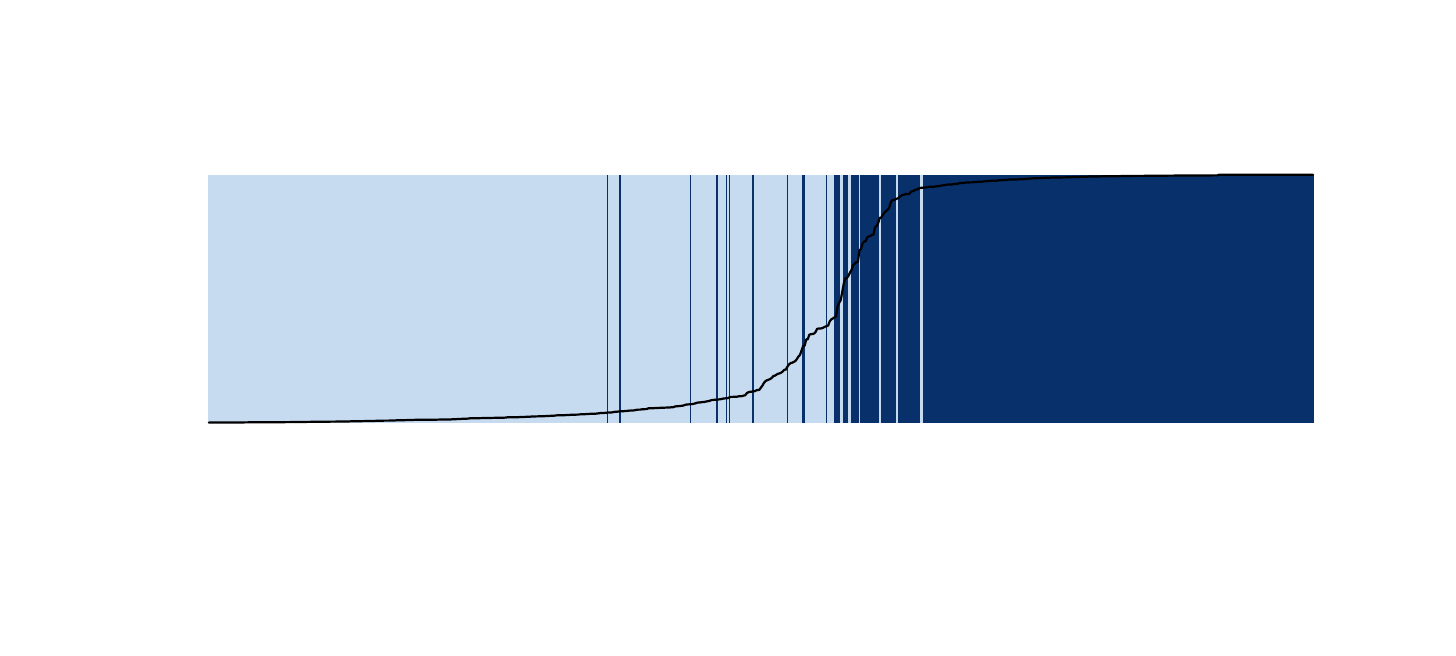
\begin{tikzpicture}[x=1pt,y=1pt]
\definecolor[named]{drawColor}{rgb}{0.00,0.00,0.00}
\definecolor[named]{fillColor}{rgb}{1.00,1.00,1.00}
\fill[color=fillColor,fill opacity=0.00,] (0,0) rectangle (505.89,216.81);
\begin{scope}
\path[clip] (  0.00,  0.00) rectangle (505.89,216.81);
\end{scope}
\begin{scope}
\path[clip] ( 49.20, 61.20) rectangle (480.69,167.61);
\definecolor[named]{fillColor}{rgb}{0.78,0.86,0.94}

\draw[fill=fillColor,draw opacity=0.00,] ( 65.18, 74.10) rectangle ( 65.75,163.67);

\draw[fill=fillColor,draw opacity=0.00,] ( 65.75, 74.10) rectangle ( 66.31,163.67);

\draw[fill=fillColor,draw opacity=0.00,] ( 66.31, 74.10) rectangle ( 66.88,163.67);

\draw[fill=fillColor,draw opacity=0.00,] ( 66.88, 74.10) rectangle ( 67.44,163.67);

\draw[fill=fillColor,draw opacity=0.00,] ( 67.44, 74.10) rectangle ( 68.01,163.67);

\draw[fill=fillColor,draw opacity=0.00,] ( 68.01, 74.10) rectangle ( 68.57,163.67);

\draw[fill=fillColor,draw opacity=0.00,] ( 68.57, 74.10) rectangle ( 69.14,163.67);

\draw[fill=fillColor,draw opacity=0.00,] ( 69.14, 74.10) rectangle ( 69.70,163.67);

\draw[fill=fillColor,draw opacity=0.00,] ( 69.70, 74.10) rectangle ( 70.27,163.67);

\draw[fill=fillColor,draw opacity=0.00,] ( 70.27, 74.10) rectangle ( 70.83,163.67);

\draw[fill=fillColor,draw opacity=0.00,] ( 70.83, 74.10) rectangle ( 71.40,163.67);

\draw[fill=fillColor,draw opacity=0.00,] ( 71.40, 74.10) rectangle ( 71.96,163.67);

\draw[fill=fillColor,draw opacity=0.00,] ( 71.96, 74.10) rectangle ( 72.53,163.67);

\draw[fill=fillColor,draw opacity=0.00,] ( 72.53, 74.10) rectangle ( 73.09,163.67);

\draw[fill=fillColor,draw opacity=0.00,] ( 73.09, 74.10) rectangle ( 73.66,163.67);

\draw[fill=fillColor,draw opacity=0.00,] ( 73.66, 74.10) rectangle ( 74.22,163.67);

\draw[fill=fillColor,draw opacity=0.00,] ( 74.22, 74.10) rectangle ( 74.79,163.67);

\draw[fill=fillColor,draw opacity=0.00,] ( 74.79, 74.10) rectangle ( 75.35,163.67);

\draw[fill=fillColor,draw opacity=0.00,] ( 75.35, 74.10) rectangle ( 75.92,163.67);

\draw[fill=fillColor,draw opacity=0.00,] ( 75.92, 74.10) rectangle ( 76.48,163.67);

\draw[fill=fillColor,draw opacity=0.00,] ( 76.48, 74.10) rectangle ( 77.05,163.67);

\draw[fill=fillColor,draw opacity=0.00,] ( 77.05, 74.10) rectangle ( 77.61,163.67);

\draw[fill=fillColor,draw opacity=0.00,] ( 77.61, 74.10) rectangle ( 78.18,163.67);

\draw[fill=fillColor,draw opacity=0.00,] ( 78.18, 74.10) rectangle ( 78.74,163.67);

\draw[fill=fillColor,draw opacity=0.00,] ( 78.74, 74.10) rectangle ( 79.31,163.67);

\draw[fill=fillColor,draw opacity=0.00,] ( 79.31, 74.10) rectangle ( 79.87,163.67);

\draw[fill=fillColor,draw opacity=0.00,] ( 79.87, 74.10) rectangle ( 80.44,163.67);

\draw[fill=fillColor,draw opacity=0.00,] ( 80.44, 74.10) rectangle ( 81.00,163.67);

\draw[fill=fillColor,draw opacity=0.00,] ( 81.00, 74.10) rectangle ( 81.57,163.67);

\draw[fill=fillColor,draw opacity=0.00,] ( 81.57, 74.10) rectangle ( 82.13,163.67);

\draw[fill=fillColor,draw opacity=0.00,] ( 82.13, 74.10) rectangle ( 82.70,163.67);

\draw[fill=fillColor,draw opacity=0.00,] ( 82.70, 74.10) rectangle ( 83.26,163.67);

\draw[fill=fillColor,draw opacity=0.00,] ( 83.26, 74.10) rectangle ( 83.83,163.67);

\draw[fill=fillColor,draw opacity=0.00,] ( 83.83, 74.10) rectangle ( 84.39,163.67);

\draw[fill=fillColor,draw opacity=0.00,] ( 84.39, 74.10) rectangle ( 84.96,163.67);

\draw[fill=fillColor,draw opacity=0.00,] ( 84.96, 74.10) rectangle ( 85.52,163.67);

\draw[fill=fillColor,draw opacity=0.00,] ( 85.52, 74.10) rectangle ( 86.09,163.67);

\draw[fill=fillColor,draw opacity=0.00,] ( 86.09, 74.10) rectangle ( 86.66,163.67);

\draw[fill=fillColor,draw opacity=0.00,] ( 86.66, 74.10) rectangle ( 87.22,163.67);

\draw[fill=fillColor,draw opacity=0.00,] ( 87.22, 74.10) rectangle ( 87.79,163.67);

\draw[fill=fillColor,draw opacity=0.00,] ( 87.79, 74.10) rectangle ( 88.35,163.67);

\draw[fill=fillColor,draw opacity=0.00,] ( 88.35, 74.10) rectangle ( 88.92,163.67);

\draw[fill=fillColor,draw opacity=0.00,] ( 88.92, 74.10) rectangle ( 89.48,163.67);

\draw[fill=fillColor,draw opacity=0.00,] ( 89.48, 74.10) rectangle ( 90.05,163.67);

\draw[fill=fillColor,draw opacity=0.00,] ( 90.05, 74.10) rectangle ( 90.61,163.67);

\draw[fill=fillColor,draw opacity=0.00,] ( 90.61, 74.10) rectangle ( 91.18,163.67);

\draw[fill=fillColor,draw opacity=0.00,] ( 91.18, 74.10) rectangle ( 91.74,163.67);

\draw[fill=fillColor,draw opacity=0.00,] ( 91.74, 74.10) rectangle ( 92.31,163.67);

\draw[fill=fillColor,draw opacity=0.00,] ( 92.31, 74.10) rectangle ( 92.87,163.67);

\draw[fill=fillColor,draw opacity=0.00,] ( 92.87, 74.10) rectangle ( 93.44,163.67);

\draw[fill=fillColor,draw opacity=0.00,] ( 93.44, 74.10) rectangle ( 94.00,163.67);

\draw[fill=fillColor,draw opacity=0.00,] ( 94.00, 74.10) rectangle ( 94.57,163.67);

\draw[fill=fillColor,draw opacity=0.00,] ( 94.57, 74.10) rectangle ( 95.13,163.67);

\draw[fill=fillColor,draw opacity=0.00,] ( 95.13, 74.10) rectangle ( 95.70,163.67);

\draw[fill=fillColor,draw opacity=0.00,] ( 95.70, 74.10) rectangle ( 96.26,163.67);

\draw[fill=fillColor,draw opacity=0.00,] ( 96.26, 74.10) rectangle ( 96.83,163.67);

\draw[fill=fillColor,draw opacity=0.00,] ( 96.83, 74.10) rectangle ( 97.39,163.67);

\draw[fill=fillColor,draw opacity=0.00,] ( 97.39, 74.10) rectangle ( 97.96,163.67);

\draw[fill=fillColor,draw opacity=0.00,] ( 97.96, 74.10) rectangle ( 98.52,163.67);

\draw[fill=fillColor,draw opacity=0.00,] ( 98.52, 74.10) rectangle ( 99.09,163.67);

\draw[fill=fillColor,draw opacity=0.00,] ( 99.09, 74.10) rectangle ( 99.65,163.67);

\draw[fill=fillColor,draw opacity=0.00,] ( 99.65, 74.10) rectangle (100.22,163.67);

\draw[fill=fillColor,draw opacity=0.00,] (100.22, 74.10) rectangle (100.78,163.67);

\draw[fill=fillColor,draw opacity=0.00,] (100.78, 74.10) rectangle (101.35,163.67);

\draw[fill=fillColor,draw opacity=0.00,] (101.35, 74.10) rectangle (101.91,163.67);

\draw[fill=fillColor,draw opacity=0.00,] (101.91, 74.10) rectangle (102.48,163.67);

\draw[fill=fillColor,draw opacity=0.00,] (102.48, 74.10) rectangle (103.04,163.67);

\draw[fill=fillColor,draw opacity=0.00,] (103.04, 74.10) rectangle (103.61,163.67);

\draw[fill=fillColor,draw opacity=0.00,] (103.61, 74.10) rectangle (104.17,163.67);

\draw[fill=fillColor,draw opacity=0.00,] (104.17, 74.10) rectangle (104.74,163.67);

\draw[fill=fillColor,draw opacity=0.00,] (104.74, 74.10) rectangle (105.30,163.67);

\draw[fill=fillColor,draw opacity=0.00,] (105.30, 74.10) rectangle (105.87,163.67);

\draw[fill=fillColor,draw opacity=0.00,] (105.87, 74.10) rectangle (106.43,163.67);

\draw[fill=fillColor,draw opacity=0.00,] (106.43, 74.10) rectangle (107.00,163.67);

\draw[fill=fillColor,draw opacity=0.00,] (107.00, 74.10) rectangle (107.56,163.67);

\draw[fill=fillColor,draw opacity=0.00,] (107.56, 74.10) rectangle (108.13,163.67);

\draw[fill=fillColor,draw opacity=0.00,] (108.13, 74.10) rectangle (108.69,163.67);

\draw[fill=fillColor,draw opacity=0.00,] (108.69, 74.10) rectangle (109.26,163.67);

\draw[fill=fillColor,draw opacity=0.00,] (109.26, 74.10) rectangle (109.82,163.67);

\draw[fill=fillColor,draw opacity=0.00,] (109.82, 74.10) rectangle (110.39,163.67);

\draw[fill=fillColor,draw opacity=0.00,] (110.39, 74.10) rectangle (110.95,163.67);

\draw[fill=fillColor,draw opacity=0.00,] (110.95, 74.10) rectangle (111.52,163.67);

\draw[fill=fillColor,draw opacity=0.00,] (111.52, 74.10) rectangle (112.08,163.67);

\draw[fill=fillColor,draw opacity=0.00,] (112.08, 74.10) rectangle (112.65,163.67);

\draw[fill=fillColor,draw opacity=0.00,] (112.65, 74.10) rectangle (113.21,163.67);

\draw[fill=fillColor,draw opacity=0.00,] (113.21, 74.10) rectangle (113.78,163.67);

\draw[fill=fillColor,draw opacity=0.00,] (113.78, 74.10) rectangle (114.35,163.67);

\draw[fill=fillColor,draw opacity=0.00,] (114.35, 74.10) rectangle (114.91,163.67);

\draw[fill=fillColor,draw opacity=0.00,] (114.91, 74.10) rectangle (115.48,163.67);

\draw[fill=fillColor,draw opacity=0.00,] (115.48, 74.10) rectangle (116.04,163.67);

\draw[fill=fillColor,draw opacity=0.00,] (116.04, 74.10) rectangle (116.61,163.67);

\draw[fill=fillColor,draw opacity=0.00,] (116.61, 74.10) rectangle (117.17,163.67);

\draw[fill=fillColor,draw opacity=0.00,] (117.17, 74.10) rectangle (117.74,163.67);

\draw[fill=fillColor,draw opacity=0.00,] (117.74, 74.10) rectangle (118.30,163.67);

\draw[fill=fillColor,draw opacity=0.00,] (118.30, 74.10) rectangle (118.87,163.67);

\draw[fill=fillColor,draw opacity=0.00,] (118.87, 74.10) rectangle (119.43,163.67);

\draw[fill=fillColor,draw opacity=0.00,] (119.43, 74.10) rectangle (120.00,163.67);

\draw[fill=fillColor,draw opacity=0.00,] (120.00, 74.10) rectangle (120.56,163.67);

\draw[fill=fillColor,draw opacity=0.00,] (120.56, 74.10) rectangle (121.13,163.67);

\draw[fill=fillColor,draw opacity=0.00,] (121.13, 74.10) rectangle (121.69,163.67);

\draw[fill=fillColor,draw opacity=0.00,] (121.69, 74.10) rectangle (122.26,163.67);

\draw[fill=fillColor,draw opacity=0.00,] (122.26, 74.10) rectangle (122.82,163.67);

\draw[fill=fillColor,draw opacity=0.00,] (122.82, 74.10) rectangle (123.39,163.67);

\draw[fill=fillColor,draw opacity=0.00,] (123.39, 74.10) rectangle (123.95,163.67);

\draw[fill=fillColor,draw opacity=0.00,] (123.95, 74.10) rectangle (124.52,163.67);

\draw[fill=fillColor,draw opacity=0.00,] (124.52, 74.10) rectangle (125.08,163.67);

\draw[fill=fillColor,draw opacity=0.00,] (125.08, 74.10) rectangle (125.65,163.67);

\draw[fill=fillColor,draw opacity=0.00,] (125.65, 74.10) rectangle (126.21,163.67);

\draw[fill=fillColor,draw opacity=0.00,] (126.21, 74.10) rectangle (126.78,163.67);

\draw[fill=fillColor,draw opacity=0.00,] (126.78, 74.10) rectangle (127.34,163.67);

\draw[fill=fillColor,draw opacity=0.00,] (127.34, 74.10) rectangle (127.91,163.67);

\draw[fill=fillColor,draw opacity=0.00,] (127.91, 74.10) rectangle (128.47,163.67);

\draw[fill=fillColor,draw opacity=0.00,] (128.47, 74.10) rectangle (129.04,163.67);

\draw[fill=fillColor,draw opacity=0.00,] (129.04, 74.10) rectangle (129.60,163.67);

\draw[fill=fillColor,draw opacity=0.00,] (129.60, 74.10) rectangle (130.17,163.67);

\draw[fill=fillColor,draw opacity=0.00,] (130.17, 74.10) rectangle (130.73,163.67);

\draw[fill=fillColor,draw opacity=0.00,] (130.73, 74.10) rectangle (131.30,163.67);

\draw[fill=fillColor,draw opacity=0.00,] (131.30, 74.10) rectangle (131.86,163.67);

\draw[fill=fillColor,draw opacity=0.00,] (131.86, 74.10) rectangle (132.43,163.67);

\draw[fill=fillColor,draw opacity=0.00,] (132.43, 74.10) rectangle (132.99,163.67);

\draw[fill=fillColor,draw opacity=0.00,] (132.99, 74.10) rectangle (133.56,163.67);

\draw[fill=fillColor,draw opacity=0.00,] (133.56, 74.10) rectangle (134.12,163.67);

\draw[fill=fillColor,draw opacity=0.00,] (134.12, 74.10) rectangle (134.69,163.67);

\draw[fill=fillColor,draw opacity=0.00,] (134.69, 74.10) rectangle (135.25,163.67);

\draw[fill=fillColor,draw opacity=0.00,] (135.25, 74.10) rectangle (135.82,163.67);

\draw[fill=fillColor,draw opacity=0.00,] (135.82, 74.10) rectangle (136.38,163.67);

\draw[fill=fillColor,draw opacity=0.00,] (136.38, 74.10) rectangle (136.95,163.67);

\draw[fill=fillColor,draw opacity=0.00,] (136.95, 74.10) rectangle (137.51,163.67);

\draw[fill=fillColor,draw opacity=0.00,] (137.51, 74.10) rectangle (138.08,163.67);

\draw[fill=fillColor,draw opacity=0.00,] (138.08, 74.10) rectangle (138.64,163.67);

\draw[fill=fillColor,draw opacity=0.00,] (138.64, 74.10) rectangle (139.21,163.67);

\draw[fill=fillColor,draw opacity=0.00,] (139.21, 74.10) rectangle (139.77,163.67);

\draw[fill=fillColor,draw opacity=0.00,] (139.77, 74.10) rectangle (140.34,163.67);

\draw[fill=fillColor,draw opacity=0.00,] (140.34, 74.10) rectangle (140.90,163.67);

\draw[fill=fillColor,draw opacity=0.00,] (140.90, 74.10) rectangle (141.47,163.67);

\draw[fill=fillColor,draw opacity=0.00,] (141.47, 74.10) rectangle (142.04,163.67);

\draw[fill=fillColor,draw opacity=0.00,] (142.04, 74.10) rectangle (142.60,163.67);

\draw[fill=fillColor,draw opacity=0.00,] (142.60, 74.10) rectangle (143.17,163.67);

\draw[fill=fillColor,draw opacity=0.00,] (143.17, 74.10) rectangle (143.73,163.67);

\draw[fill=fillColor,draw opacity=0.00,] (143.73, 74.10) rectangle (144.30,163.67);

\draw[fill=fillColor,draw opacity=0.00,] (144.30, 74.10) rectangle (144.86,163.67);

\draw[fill=fillColor,draw opacity=0.00,] (144.86, 74.10) rectangle (145.43,163.67);

\draw[fill=fillColor,draw opacity=0.00,] (145.43, 74.10) rectangle (145.99,163.67);

\draw[fill=fillColor,draw opacity=0.00,] (145.99, 74.10) rectangle (146.56,163.67);

\draw[fill=fillColor,draw opacity=0.00,] (146.56, 74.10) rectangle (147.12,163.67);

\draw[fill=fillColor,draw opacity=0.00,] (147.12, 74.10) rectangle (147.69,163.67);

\draw[fill=fillColor,draw opacity=0.00,] (147.69, 74.10) rectangle (148.25,163.67);

\draw[fill=fillColor,draw opacity=0.00,] (148.25, 74.10) rectangle (148.82,163.67);

\draw[fill=fillColor,draw opacity=0.00,] (148.82, 74.10) rectangle (149.38,163.67);

\draw[fill=fillColor,draw opacity=0.00,] (149.38, 74.10) rectangle (149.95,163.67);

\draw[fill=fillColor,draw opacity=0.00,] (149.95, 74.10) rectangle (150.51,163.67);

\draw[fill=fillColor,draw opacity=0.00,] (150.51, 74.10) rectangle (151.08,163.67);

\draw[fill=fillColor,draw opacity=0.00,] (151.08, 74.10) rectangle (151.64,163.67);

\draw[fill=fillColor,draw opacity=0.00,] (151.64, 74.10) rectangle (152.21,163.67);

\draw[fill=fillColor,draw opacity=0.00,] (152.21, 74.10) rectangle (152.77,163.67);

\draw[fill=fillColor,draw opacity=0.00,] (152.77, 74.10) rectangle (153.34,163.67);

\draw[fill=fillColor,draw opacity=0.00,] (153.34, 74.10) rectangle (153.90,163.67);

\draw[fill=fillColor,draw opacity=0.00,] (153.90, 74.10) rectangle (154.47,163.67);

\draw[fill=fillColor,draw opacity=0.00,] (154.47, 74.10) rectangle (155.03,163.67);

\draw[fill=fillColor,draw opacity=0.00,] (155.03, 74.10) rectangle (155.60,163.67);

\draw[fill=fillColor,draw opacity=0.00,] (155.60, 74.10) rectangle (156.16,163.67);

\draw[fill=fillColor,draw opacity=0.00,] (156.16, 74.10) rectangle (156.73,163.67);

\draw[fill=fillColor,draw opacity=0.00,] (156.73, 74.10) rectangle (157.29,163.67);

\draw[fill=fillColor,draw opacity=0.00,] (157.29, 74.10) rectangle (157.86,163.67);

\draw[fill=fillColor,draw opacity=0.00,] (157.86, 74.10) rectangle (158.42,163.67);

\draw[fill=fillColor,draw opacity=0.00,] (158.42, 74.10) rectangle (158.99,163.67);

\draw[fill=fillColor,draw opacity=0.00,] (158.99, 74.10) rectangle (159.55,163.67);

\draw[fill=fillColor,draw opacity=0.00,] (159.55, 74.10) rectangle (160.12,163.67);

\draw[fill=fillColor,draw opacity=0.00,] (160.12, 74.10) rectangle (160.68,163.67);

\draw[fill=fillColor,draw opacity=0.00,] (160.68, 74.10) rectangle (161.25,163.67);

\draw[fill=fillColor,draw opacity=0.00,] (161.25, 74.10) rectangle (161.81,163.67);

\draw[fill=fillColor,draw opacity=0.00,] (161.81, 74.10) rectangle (162.38,163.67);

\draw[fill=fillColor,draw opacity=0.00,] (162.38, 74.10) rectangle (162.94,163.67);

\draw[fill=fillColor,draw opacity=0.00,] (162.94, 74.10) rectangle (163.51,163.67);

\draw[fill=fillColor,draw opacity=0.00,] (163.51, 74.10) rectangle (164.07,163.67);

\draw[fill=fillColor,draw opacity=0.00,] (164.07, 74.10) rectangle (164.64,163.67);

\draw[fill=fillColor,draw opacity=0.00,] (164.64, 74.10) rectangle (165.20,163.67);

\draw[fill=fillColor,draw opacity=0.00,] (165.20, 74.10) rectangle (165.77,163.67);

\draw[fill=fillColor,draw opacity=0.00,] (165.77, 74.10) rectangle (166.33,163.67);

\draw[fill=fillColor,draw opacity=0.00,] (166.33, 74.10) rectangle (166.90,163.67);

\draw[fill=fillColor,draw opacity=0.00,] (166.90, 74.10) rectangle (167.46,163.67);

\draw[fill=fillColor,draw opacity=0.00,] (167.46, 74.10) rectangle (168.03,163.67);

\draw[fill=fillColor,draw opacity=0.00,] (168.03, 74.10) rectangle (168.59,163.67);

\draw[fill=fillColor,draw opacity=0.00,] (168.59, 74.10) rectangle (169.16,163.67);

\draw[fill=fillColor,draw opacity=0.00,] (169.16, 74.10) rectangle (169.73,163.67);

\draw[fill=fillColor,draw opacity=0.00,] (169.73, 74.10) rectangle (170.29,163.67);

\draw[fill=fillColor,draw opacity=0.00,] (170.29, 74.10) rectangle (170.86,163.67);

\draw[fill=fillColor,draw opacity=0.00,] (170.86, 74.10) rectangle (171.42,163.67);

\draw[fill=fillColor,draw opacity=0.00,] (171.42, 74.10) rectangle (171.99,163.67);

\draw[fill=fillColor,draw opacity=0.00,] (171.99, 74.10) rectangle (172.55,163.67);

\draw[fill=fillColor,draw opacity=0.00,] (172.55, 74.10) rectangle (173.12,163.67);

\draw[fill=fillColor,draw opacity=0.00,] (173.12, 74.10) rectangle (173.68,163.67);

\draw[fill=fillColor,draw opacity=0.00,] (173.68, 74.10) rectangle (174.25,163.67);

\draw[fill=fillColor,draw opacity=0.00,] (174.25, 74.10) rectangle (174.81,163.67);

\draw[fill=fillColor,draw opacity=0.00,] (174.81, 74.10) rectangle (175.38,163.67);

\draw[fill=fillColor,draw opacity=0.00,] (175.38, 74.10) rectangle (175.94,163.67);

\draw[fill=fillColor,draw opacity=0.00,] (175.94, 74.10) rectangle (176.51,163.67);

\draw[fill=fillColor,draw opacity=0.00,] (176.51, 74.10) rectangle (177.07,163.67);

\draw[fill=fillColor,draw opacity=0.00,] (177.07, 74.10) rectangle (177.64,163.67);

\draw[fill=fillColor,draw opacity=0.00,] (177.64, 74.10) rectangle (178.20,163.67);

\draw[fill=fillColor,draw opacity=0.00,] (178.20, 74.10) rectangle (178.77,163.67);

\draw[fill=fillColor,draw opacity=0.00,] (178.77, 74.10) rectangle (179.33,163.67);

\draw[fill=fillColor,draw opacity=0.00,] (179.33, 74.10) rectangle (179.90,163.67);

\draw[fill=fillColor,draw opacity=0.00,] (179.90, 74.10) rectangle (180.46,163.67);

\draw[fill=fillColor,draw opacity=0.00,] (180.46, 74.10) rectangle (181.03,163.67);

\draw[fill=fillColor,draw opacity=0.00,] (181.03, 74.10) rectangle (181.59,163.67);

\draw[fill=fillColor,draw opacity=0.00,] (181.59, 74.10) rectangle (182.16,163.67);

\draw[fill=fillColor,draw opacity=0.00,] (182.16, 74.10) rectangle (182.72,163.67);

\draw[fill=fillColor,draw opacity=0.00,] (182.72, 74.10) rectangle (183.29,163.67);

\draw[fill=fillColor,draw opacity=0.00,] (183.29, 74.10) rectangle (183.85,163.67);

\draw[fill=fillColor,draw opacity=0.00,] (183.85, 74.10) rectangle (184.42,163.67);

\draw[fill=fillColor,draw opacity=0.00,] (184.42, 74.10) rectangle (184.98,163.67);

\draw[fill=fillColor,draw opacity=0.00,] (184.98, 74.10) rectangle (185.55,163.67);

\draw[fill=fillColor,draw opacity=0.00,] (185.55, 74.10) rectangle (186.11,163.67);

\draw[fill=fillColor,draw opacity=0.00,] (186.11, 74.10) rectangle (186.68,163.67);

\draw[fill=fillColor,draw opacity=0.00,] (186.68, 74.10) rectangle (187.24,163.67);

\draw[fill=fillColor,draw opacity=0.00,] (187.24, 74.10) rectangle (187.81,163.67);

\draw[fill=fillColor,draw opacity=0.00,] (187.81, 74.10) rectangle (188.37,163.67);

\draw[fill=fillColor,draw opacity=0.00,] (188.37, 74.10) rectangle (188.94,163.67);

\draw[fill=fillColor,draw opacity=0.00,] (188.94, 74.10) rectangle (189.50,163.67);

\draw[fill=fillColor,draw opacity=0.00,] (189.50, 74.10) rectangle (190.07,163.67);

\draw[fill=fillColor,draw opacity=0.00,] (190.07, 74.10) rectangle (190.63,163.67);

\draw[fill=fillColor,draw opacity=0.00,] (190.63, 74.10) rectangle (191.20,163.67);

\draw[fill=fillColor,draw opacity=0.00,] (191.20, 74.10) rectangle (191.76,163.67);

\draw[fill=fillColor,draw opacity=0.00,] (191.76, 74.10) rectangle (192.33,163.67);

\draw[fill=fillColor,draw opacity=0.00,] (192.33, 74.10) rectangle (192.89,163.67);

\draw[fill=fillColor,draw opacity=0.00,] (192.89, 74.10) rectangle (193.46,163.67);

\draw[fill=fillColor,draw opacity=0.00,] (193.46, 74.10) rectangle (194.02,163.67);

\draw[fill=fillColor,draw opacity=0.00,] (194.02, 74.10) rectangle (194.59,163.67);

\draw[fill=fillColor,draw opacity=0.00,] (194.59, 74.10) rectangle (195.15,163.67);

\draw[fill=fillColor,draw opacity=0.00,] (195.15, 74.10) rectangle (195.72,163.67);

\draw[fill=fillColor,draw opacity=0.00,] (195.72, 74.10) rectangle (196.28,163.67);

\draw[fill=fillColor,draw opacity=0.00,] (196.28, 74.10) rectangle (196.85,163.67);

\draw[fill=fillColor,draw opacity=0.00,] (196.85, 74.10) rectangle (197.42,163.67);

\draw[fill=fillColor,draw opacity=0.00,] (197.42, 74.10) rectangle (197.98,163.67);

\draw[fill=fillColor,draw opacity=0.00,] (197.98, 74.10) rectangle (198.55,163.67);

\draw[fill=fillColor,draw opacity=0.00,] (198.55, 74.10) rectangle (199.11,163.67);

\draw[fill=fillColor,draw opacity=0.00,] (199.11, 74.10) rectangle (199.68,163.67);

\draw[fill=fillColor,draw opacity=0.00,] (199.68, 74.10) rectangle (200.24,163.67);

\draw[fill=fillColor,draw opacity=0.00,] (200.24, 74.10) rectangle (200.81,163.67);

\draw[fill=fillColor,draw opacity=0.00,] (200.81, 74.10) rectangle (201.37,163.67);

\draw[fill=fillColor,draw opacity=0.00,] (201.37, 74.10) rectangle (201.94,163.67);

\draw[fill=fillColor,draw opacity=0.00,] (201.94, 74.10) rectangle (202.50,163.67);

\draw[fill=fillColor,draw opacity=0.00,] (202.50, 74.10) rectangle (203.07,163.67);

\draw[fill=fillColor,draw opacity=0.00,] (203.07, 74.10) rectangle (203.63,163.67);

\draw[fill=fillColor,draw opacity=0.00,] (203.63, 74.10) rectangle (204.20,163.67);

\draw[fill=fillColor,draw opacity=0.00,] (204.20, 74.10) rectangle (204.76,163.67);

\draw[fill=fillColor,draw opacity=0.00,] (204.76, 74.10) rectangle (205.33,163.67);

\draw[fill=fillColor,draw opacity=0.00,] (205.33, 74.10) rectangle (205.89,163.67);

\draw[fill=fillColor,draw opacity=0.00,] (205.89, 74.10) rectangle (206.46,163.67);

\draw[fill=fillColor,draw opacity=0.00,] (206.46, 74.10) rectangle (207.02,163.67);

\draw[fill=fillColor,draw opacity=0.00,] (207.02, 74.10) rectangle (207.59,163.67);

\draw[fill=fillColor,draw opacity=0.00,] (207.59, 74.10) rectangle (208.15,163.67);

\draw[fill=fillColor,draw opacity=0.00,] (208.15, 74.10) rectangle (208.72,163.67);

\draw[fill=fillColor,draw opacity=0.00,] (208.72, 74.10) rectangle (209.28,163.67);
\definecolor[named]{fillColor}{rgb}{0.03,0.19,0.42}

\draw[fill=fillColor,draw opacity=0.00,] (209.28, 74.10) rectangle (209.85,163.67);
\definecolor[named]{fillColor}{rgb}{0.78,0.86,0.94}

\draw[fill=fillColor,draw opacity=0.00,] (209.85, 74.10) rectangle (210.41,163.67);

\draw[fill=fillColor,draw opacity=0.00,] (210.41, 74.10) rectangle (210.98,163.67);

\draw[fill=fillColor,draw opacity=0.00,] (210.98, 74.10) rectangle (211.54,163.67);

\draw[fill=fillColor,draw opacity=0.00,] (211.54, 74.10) rectangle (212.11,163.67);

\draw[fill=fillColor,draw opacity=0.00,] (212.11, 74.10) rectangle (212.67,163.67);

\draw[fill=fillColor,draw opacity=0.00,] (212.67, 74.10) rectangle (213.24,163.67);

\draw[fill=fillColor,draw opacity=0.00,] (213.24, 74.10) rectangle (213.80,163.67);
\definecolor[named]{fillColor}{rgb}{0.03,0.19,0.42}

\draw[fill=fillColor,draw opacity=0.00,] (213.80, 74.10) rectangle (214.37,163.67);
\definecolor[named]{fillColor}{rgb}{0.78,0.86,0.94}

\draw[fill=fillColor,draw opacity=0.00,] (214.37, 74.10) rectangle (214.93,163.67);

\draw[fill=fillColor,draw opacity=0.00,] (214.93, 74.10) rectangle (215.50,163.67);

\draw[fill=fillColor,draw opacity=0.00,] (215.50, 74.10) rectangle (216.06,163.67);

\draw[fill=fillColor,draw opacity=0.00,] (216.06, 74.10) rectangle (216.63,163.67);

\draw[fill=fillColor,draw opacity=0.00,] (216.63, 74.10) rectangle (217.19,163.67);

\draw[fill=fillColor,draw opacity=0.00,] (217.19, 74.10) rectangle (217.76,163.67);

\draw[fill=fillColor,draw opacity=0.00,] (217.76, 74.10) rectangle (218.32,163.67);

\draw[fill=fillColor,draw opacity=0.00,] (218.32, 74.10) rectangle (218.89,163.67);

\draw[fill=fillColor,draw opacity=0.00,] (218.89, 74.10) rectangle (219.45,163.67);

\draw[fill=fillColor,draw opacity=0.00,] (219.45, 74.10) rectangle (220.02,163.67);

\draw[fill=fillColor,draw opacity=0.00,] (220.02, 74.10) rectangle (220.58,163.67);

\draw[fill=fillColor,draw opacity=0.00,] (220.58, 74.10) rectangle (221.15,163.67);

\draw[fill=fillColor,draw opacity=0.00,] (221.15, 74.10) rectangle (221.71,163.67);

\draw[fill=fillColor,draw opacity=0.00,] (221.71, 74.10) rectangle (222.28,163.67);

\draw[fill=fillColor,draw opacity=0.00,] (222.28, 74.10) rectangle (222.84,163.67);

\draw[fill=fillColor,draw opacity=0.00,] (222.84, 74.10) rectangle (223.41,163.67);

\draw[fill=fillColor,draw opacity=0.00,] (223.41, 74.10) rectangle (223.98,163.67);

\draw[fill=fillColor,draw opacity=0.00,] (223.98, 74.10) rectangle (224.54,163.67);

\draw[fill=fillColor,draw opacity=0.00,] (224.54, 74.10) rectangle (225.11,163.67);

\draw[fill=fillColor,draw opacity=0.00,] (225.11, 74.10) rectangle (225.67,163.67);

\draw[fill=fillColor,draw opacity=0.00,] (225.67, 74.10) rectangle (226.24,163.67);

\draw[fill=fillColor,draw opacity=0.00,] (226.24, 74.10) rectangle (226.80,163.67);

\draw[fill=fillColor,draw opacity=0.00,] (226.80, 74.10) rectangle (227.37,163.67);

\draw[fill=fillColor,draw opacity=0.00,] (227.37, 74.10) rectangle (227.93,163.67);

\draw[fill=fillColor,draw opacity=0.00,] (227.93, 74.10) rectangle (228.50,163.67);

\draw[fill=fillColor,draw opacity=0.00,] (228.50, 74.10) rectangle (229.06,163.67);

\draw[fill=fillColor,draw opacity=0.00,] (229.06, 74.10) rectangle (229.63,163.67);

\draw[fill=fillColor,draw opacity=0.00,] (229.63, 74.10) rectangle (230.19,163.67);

\draw[fill=fillColor,draw opacity=0.00,] (230.19, 74.10) rectangle (230.76,163.67);

\draw[fill=fillColor,draw opacity=0.00,] (230.76, 74.10) rectangle (231.32,163.67);

\draw[fill=fillColor,draw opacity=0.00,] (231.32, 74.10) rectangle (231.89,163.67);

\draw[fill=fillColor,draw opacity=0.00,] (231.89, 74.10) rectangle (232.45,163.67);

\draw[fill=fillColor,draw opacity=0.00,] (232.45, 74.10) rectangle (233.02,163.67);

\draw[fill=fillColor,draw opacity=0.00,] (233.02, 74.10) rectangle (233.58,163.67);

\draw[fill=fillColor,draw opacity=0.00,] (233.58, 74.10) rectangle (234.15,163.67);

\draw[fill=fillColor,draw opacity=0.00,] (234.15, 74.10) rectangle (234.71,163.67);

\draw[fill=fillColor,draw opacity=0.00,] (234.71, 74.10) rectangle (235.28,163.67);

\draw[fill=fillColor,draw opacity=0.00,] (235.28, 74.10) rectangle (235.84,163.67);

\draw[fill=fillColor,draw opacity=0.00,] (235.84, 74.10) rectangle (236.41,163.67);

\draw[fill=fillColor,draw opacity=0.00,] (236.41, 74.10) rectangle (236.97,163.67);

\draw[fill=fillColor,draw opacity=0.00,] (236.97, 74.10) rectangle (237.54,163.67);

\draw[fill=fillColor,draw opacity=0.00,] (237.54, 74.10) rectangle (238.10,163.67);

\draw[fill=fillColor,draw opacity=0.00,] (238.10, 74.10) rectangle (238.67,163.67);

\draw[fill=fillColor,draw opacity=0.00,] (238.67, 74.10) rectangle (239.23,163.67);
\definecolor[named]{fillColor}{rgb}{0.03,0.19,0.42}

\draw[fill=fillColor,draw opacity=0.00,] (239.23, 74.10) rectangle (239.80,163.67);
\definecolor[named]{fillColor}{rgb}{0.78,0.86,0.94}

\draw[fill=fillColor,draw opacity=0.00,] (239.80, 74.10) rectangle (240.36,163.67);

\draw[fill=fillColor,draw opacity=0.00,] (240.36, 74.10) rectangle (240.93,163.67);

\draw[fill=fillColor,draw opacity=0.00,] (240.93, 74.10) rectangle (241.49,163.67);

\draw[fill=fillColor,draw opacity=0.00,] (241.49, 74.10) rectangle (242.06,163.67);

\draw[fill=fillColor,draw opacity=0.00,] (242.06, 74.10) rectangle (242.62,163.67);

\draw[fill=fillColor,draw opacity=0.00,] (242.62, 74.10) rectangle (243.19,163.67);

\draw[fill=fillColor,draw opacity=0.00,] (243.19, 74.10) rectangle (243.75,163.67);

\draw[fill=fillColor,draw opacity=0.00,] (243.75, 74.10) rectangle (244.32,163.67);

\draw[fill=fillColor,draw opacity=0.00,] (244.32, 74.10) rectangle (244.88,163.67);

\draw[fill=fillColor,draw opacity=0.00,] (244.88, 74.10) rectangle (245.45,163.67);

\draw[fill=fillColor,draw opacity=0.00,] (245.45, 74.10) rectangle (246.01,163.67);

\draw[fill=fillColor,draw opacity=0.00,] (246.01, 74.10) rectangle (246.58,163.67);

\draw[fill=fillColor,draw opacity=0.00,] (246.58, 74.10) rectangle (247.14,163.67);

\draw[fill=fillColor,draw opacity=0.00,] (247.14, 74.10) rectangle (247.71,163.67);

\draw[fill=fillColor,draw opacity=0.00,] (247.71, 74.10) rectangle (248.27,163.67);

\draw[fill=fillColor,draw opacity=0.00,] (248.27, 74.10) rectangle (248.84,163.67);
\definecolor[named]{fillColor}{rgb}{0.03,0.19,0.42}

\draw[fill=fillColor,draw opacity=0.00,] (248.84, 74.10) rectangle (249.40,163.67);
\definecolor[named]{fillColor}{rgb}{0.78,0.86,0.94}

\draw[fill=fillColor,draw opacity=0.00,] (249.40, 74.10) rectangle (249.97,163.67);

\draw[fill=fillColor,draw opacity=0.00,] (249.97, 74.10) rectangle (250.53,163.67);

\draw[fill=fillColor,draw opacity=0.00,] (250.53, 74.10) rectangle (251.10,163.67);

\draw[fill=fillColor,draw opacity=0.00,] (251.10, 74.10) rectangle (251.67,163.67);

\draw[fill=fillColor,draw opacity=0.00,] (251.67, 74.10) rectangle (252.23,163.67);
\definecolor[named]{fillColor}{rgb}{0.03,0.19,0.42}

\draw[fill=fillColor,draw opacity=0.00,] (252.23, 74.10) rectangle (252.80,163.67);
\definecolor[named]{fillColor}{rgb}{0.78,0.86,0.94}

\draw[fill=fillColor,draw opacity=0.00,] (252.80, 74.10) rectangle (253.36,163.67);
\definecolor[named]{fillColor}{rgb}{0.03,0.19,0.42}

\draw[fill=fillColor,draw opacity=0.00,] (253.36, 74.10) rectangle (253.93,163.67);
\definecolor[named]{fillColor}{rgb}{0.78,0.86,0.94}

\draw[fill=fillColor,draw opacity=0.00,] (253.93, 74.10) rectangle (254.49,163.67);

\draw[fill=fillColor,draw opacity=0.00,] (254.49, 74.10) rectangle (255.06,163.67);

\draw[fill=fillColor,draw opacity=0.00,] (255.06, 74.10) rectangle (255.62,163.67);

\draw[fill=fillColor,draw opacity=0.00,] (255.62, 74.10) rectangle (256.19,163.67);

\draw[fill=fillColor,draw opacity=0.00,] (256.19, 74.10) rectangle (256.75,163.67);

\draw[fill=fillColor,draw opacity=0.00,] (256.75, 74.10) rectangle (257.32,163.67);

\draw[fill=fillColor,draw opacity=0.00,] (257.32, 74.10) rectangle (257.88,163.67);

\draw[fill=fillColor,draw opacity=0.00,] (257.88, 74.10) rectangle (258.45,163.67);

\draw[fill=fillColor,draw opacity=0.00,] (258.45, 74.10) rectangle (259.01,163.67);

\draw[fill=fillColor,draw opacity=0.00,] (259.01, 74.10) rectangle (259.58,163.67);

\draw[fill=fillColor,draw opacity=0.00,] (259.58, 74.10) rectangle (260.14,163.67);

\draw[fill=fillColor,draw opacity=0.00,] (260.14, 74.10) rectangle (260.71,163.67);

\draw[fill=fillColor,draw opacity=0.00,] (260.71, 74.10) rectangle (261.27,163.67);

\draw[fill=fillColor,draw opacity=0.00,] (261.27, 74.10) rectangle (261.84,163.67);
\definecolor[named]{fillColor}{rgb}{0.03,0.19,0.42}

\draw[fill=fillColor,draw opacity=0.00,] (261.84, 74.10) rectangle (262.40,163.67);
\definecolor[named]{fillColor}{rgb}{0.78,0.86,0.94}

\draw[fill=fillColor,draw opacity=0.00,] (262.40, 74.10) rectangle (262.97,163.67);

\draw[fill=fillColor,draw opacity=0.00,] (262.97, 74.10) rectangle (263.53,163.67);

\draw[fill=fillColor,draw opacity=0.00,] (263.53, 74.10) rectangle (264.10,163.67);

\draw[fill=fillColor,draw opacity=0.00,] (264.10, 74.10) rectangle (264.66,163.67);

\draw[fill=fillColor,draw opacity=0.00,] (264.66, 74.10) rectangle (265.23,163.67);

\draw[fill=fillColor,draw opacity=0.00,] (265.23, 74.10) rectangle (265.79,163.67);

\draw[fill=fillColor,draw opacity=0.00,] (265.79, 74.10) rectangle (266.36,163.67);

\draw[fill=fillColor,draw opacity=0.00,] (266.36, 74.10) rectangle (266.92,163.67);

\draw[fill=fillColor,draw opacity=0.00,] (266.92, 74.10) rectangle (267.49,163.67);

\draw[fill=fillColor,draw opacity=0.00,] (267.49, 74.10) rectangle (268.05,163.67);

\draw[fill=fillColor,draw opacity=0.00,] (268.05, 74.10) rectangle (268.62,163.67);

\draw[fill=fillColor,draw opacity=0.00,] (268.62, 74.10) rectangle (269.18,163.67);

\draw[fill=fillColor,draw opacity=0.00,] (269.18, 74.10) rectangle (269.75,163.67);

\draw[fill=fillColor,draw opacity=0.00,] (269.75, 74.10) rectangle (270.31,163.67);

\draw[fill=fillColor,draw opacity=0.00,] (270.31, 74.10) rectangle (270.88,163.67);

\draw[fill=fillColor,draw opacity=0.00,] (270.88, 74.10) rectangle (271.44,163.67);

\draw[fill=fillColor,draw opacity=0.00,] (271.44, 74.10) rectangle (272.01,163.67);

\draw[fill=fillColor,draw opacity=0.00,] (272.01, 74.10) rectangle (272.57,163.67);

\draw[fill=fillColor,draw opacity=0.00,] (272.57, 74.10) rectangle (273.14,163.67);

\draw[fill=fillColor,draw opacity=0.00,] (273.14, 74.10) rectangle (273.70,163.67);

\draw[fill=fillColor,draw opacity=0.00,] (273.70, 74.10) rectangle (274.27,163.67);
\definecolor[named]{fillColor}{rgb}{0.03,0.19,0.42}

\draw[fill=fillColor,draw opacity=0.00,] (274.27, 74.10) rectangle (274.83,163.67);
\definecolor[named]{fillColor}{rgb}{0.78,0.86,0.94}

\draw[fill=fillColor,draw opacity=0.00,] (274.83, 74.10) rectangle (275.40,163.67);

\draw[fill=fillColor,draw opacity=0.00,] (275.40, 74.10) rectangle (275.96,163.67);

\draw[fill=fillColor,draw opacity=0.00,] (275.96, 74.10) rectangle (276.53,163.67);

\draw[fill=fillColor,draw opacity=0.00,] (276.53, 74.10) rectangle (277.09,163.67);

\draw[fill=fillColor,draw opacity=0.00,] (277.09, 74.10) rectangle (277.66,163.67);

\draw[fill=fillColor,draw opacity=0.00,] (277.66, 74.10) rectangle (278.22,163.67);

\draw[fill=fillColor,draw opacity=0.00,] (278.22, 74.10) rectangle (278.79,163.67);

\draw[fill=fillColor,draw opacity=0.00,] (278.79, 74.10) rectangle (279.36,163.67);

\draw[fill=fillColor,draw opacity=0.00,] (279.36, 74.10) rectangle (279.92,163.67);
\definecolor[named]{fillColor}{rgb}{0.03,0.19,0.42}

\draw[fill=fillColor,draw opacity=0.00,] (279.92, 74.10) rectangle (280.49,163.67);

\draw[fill=fillColor,draw opacity=0.00,] (280.49, 74.10) rectangle (281.05,163.67);
\definecolor[named]{fillColor}{rgb}{0.78,0.86,0.94}

\draw[fill=fillColor,draw opacity=0.00,] (281.05, 74.10) rectangle (281.62,163.67);

\draw[fill=fillColor,draw opacity=0.00,] (281.62, 74.10) rectangle (282.18,163.67);

\draw[fill=fillColor,draw opacity=0.00,] (282.18, 74.10) rectangle (282.75,163.67);

\draw[fill=fillColor,draw opacity=0.00,] (282.75, 74.10) rectangle (283.31,163.67);

\draw[fill=fillColor,draw opacity=0.00,] (283.31, 74.10) rectangle (283.88,163.67);

\draw[fill=fillColor,draw opacity=0.00,] (283.88, 74.10) rectangle (284.44,163.67);

\draw[fill=fillColor,draw opacity=0.00,] (284.44, 74.10) rectangle (285.01,163.67);

\draw[fill=fillColor,draw opacity=0.00,] (285.01, 74.10) rectangle (285.57,163.67);

\draw[fill=fillColor,draw opacity=0.00,] (285.57, 74.10) rectangle (286.14,163.67);

\draw[fill=fillColor,draw opacity=0.00,] (286.14, 74.10) rectangle (286.70,163.67);

\draw[fill=fillColor,draw opacity=0.00,] (286.70, 74.10) rectangle (287.27,163.67);

\draw[fill=fillColor,draw opacity=0.00,] (287.27, 74.10) rectangle (287.83,163.67);

\draw[fill=fillColor,draw opacity=0.00,] (287.83, 74.10) rectangle (288.40,163.67);
\definecolor[named]{fillColor}{rgb}{0.03,0.19,0.42}

\draw[fill=fillColor,draw opacity=0.00,] (288.40, 74.10) rectangle (288.96,163.67);
\definecolor[named]{fillColor}{rgb}{0.78,0.86,0.94}

\draw[fill=fillColor,draw opacity=0.00,] (288.96, 74.10) rectangle (289.53,163.67);

\draw[fill=fillColor,draw opacity=0.00,] (289.53, 74.10) rectangle (290.09,163.67);

\draw[fill=fillColor,draw opacity=0.00,] (290.09, 74.10) rectangle (290.66,163.67);

\draw[fill=fillColor,draw opacity=0.00,] (290.66, 74.10) rectangle (291.22,163.67);
\definecolor[named]{fillColor}{rgb}{0.03,0.19,0.42}

\draw[fill=fillColor,draw opacity=0.00,] (291.22, 74.10) rectangle (291.79,163.67);

\draw[fill=fillColor,draw opacity=0.00,] (291.79, 74.10) rectangle (292.35,163.67);

\draw[fill=fillColor,draw opacity=0.00,] (292.35, 74.10) rectangle (292.92,163.67);

\draw[fill=fillColor,draw opacity=0.00,] (292.92, 74.10) rectangle (293.48,163.67);
\definecolor[named]{fillColor}{rgb}{0.78,0.86,0.94}

\draw[fill=fillColor,draw opacity=0.00,] (293.48, 74.10) rectangle (294.05,163.67);

\draw[fill=fillColor,draw opacity=0.00,] (294.05, 74.10) rectangle (294.61,163.67);
\definecolor[named]{fillColor}{rgb}{0.03,0.19,0.42}

\draw[fill=fillColor,draw opacity=0.00,] (294.61, 74.10) rectangle (295.18,163.67);

\draw[fill=fillColor,draw opacity=0.00,] (295.18, 74.10) rectangle (295.74,163.67);

\draw[fill=fillColor,draw opacity=0.00,] (295.74, 74.10) rectangle (296.31,163.67);
\definecolor[named]{fillColor}{rgb}{0.78,0.86,0.94}

\draw[fill=fillColor,draw opacity=0.00,] (296.31, 74.10) rectangle (296.87,163.67);

\draw[fill=fillColor,draw opacity=0.00,] (296.87, 74.10) rectangle (297.44,163.67);
\definecolor[named]{fillColor}{rgb}{0.03,0.19,0.42}

\draw[fill=fillColor,draw opacity=0.00,] (297.44, 74.10) rectangle (298.00,163.67);

\draw[fill=fillColor,draw opacity=0.00,] (298.00, 74.10) rectangle (298.57,163.67);

\draw[fill=fillColor,draw opacity=0.00,] (298.57, 74.10) rectangle (299.13,163.67);

\draw[fill=fillColor,draw opacity=0.00,] (299.13, 74.10) rectangle (299.70,163.67);

\draw[fill=fillColor,draw opacity=0.00,] (299.70, 74.10) rectangle (300.26,163.67);
\definecolor[named]{fillColor}{rgb}{0.78,0.86,0.94}

\draw[fill=fillColor,draw opacity=0.00,] (300.26, 74.10) rectangle (300.83,163.67);
\definecolor[named]{fillColor}{rgb}{0.03,0.19,0.42}

\draw[fill=fillColor,draw opacity=0.00,] (300.83, 74.10) rectangle (301.39,163.67);

\draw[fill=fillColor,draw opacity=0.00,] (301.39, 74.10) rectangle (301.96,163.67);

\draw[fill=fillColor,draw opacity=0.00,] (301.96, 74.10) rectangle (302.52,163.67);

\draw[fill=fillColor,draw opacity=0.00,] (302.52, 74.10) rectangle (303.09,163.67);

\draw[fill=fillColor,draw opacity=0.00,] (303.09, 74.10) rectangle (303.65,163.67);

\draw[fill=fillColor,draw opacity=0.00,] (303.65, 74.10) rectangle (304.22,163.67);

\draw[fill=fillColor,draw opacity=0.00,] (304.22, 74.10) rectangle (304.78,163.67);

\draw[fill=fillColor,draw opacity=0.00,] (304.78, 74.10) rectangle (305.35,163.67);

\draw[fill=fillColor,draw opacity=0.00,] (305.35, 74.10) rectangle (305.91,163.67);

\draw[fill=fillColor,draw opacity=0.00,] (305.91, 74.10) rectangle (306.48,163.67);

\draw[fill=fillColor,draw opacity=0.00,] (306.48, 74.10) rectangle (307.05,163.67);

\draw[fill=fillColor,draw opacity=0.00,] (307.05, 74.10) rectangle (307.61,163.67);
\definecolor[named]{fillColor}{rgb}{0.78,0.86,0.94}

\draw[fill=fillColor,draw opacity=0.00,] (307.61, 74.10) rectangle (308.18,163.67);
\definecolor[named]{fillColor}{rgb}{0.03,0.19,0.42}

\draw[fill=fillColor,draw opacity=0.00,] (308.18, 74.10) rectangle (308.74,163.67);

\draw[fill=fillColor,draw opacity=0.00,] (308.74, 74.10) rectangle (309.31,163.67);

\draw[fill=fillColor,draw opacity=0.00,] (309.31, 74.10) rectangle (309.87,163.67);

\draw[fill=fillColor,draw opacity=0.00,] (309.87, 74.10) rectangle (310.44,163.67);

\draw[fill=fillColor,draw opacity=0.00,] (310.44, 74.10) rectangle (311.00,163.67);

\draw[fill=fillColor,draw opacity=0.00,] (311.00, 74.10) rectangle (311.57,163.67);

\draw[fill=fillColor,draw opacity=0.00,] (311.57, 74.10) rectangle (312.13,163.67);

\draw[fill=fillColor,draw opacity=0.00,] (312.13, 74.10) rectangle (312.70,163.67);

\draw[fill=fillColor,draw opacity=0.00,] (312.70, 74.10) rectangle (313.26,163.67);

\draw[fill=fillColor,draw opacity=0.00,] (313.26, 74.10) rectangle (313.83,163.67);
\definecolor[named]{fillColor}{rgb}{0.78,0.86,0.94}

\draw[fill=fillColor,draw opacity=0.00,] (313.83, 74.10) rectangle (314.39,163.67);
\definecolor[named]{fillColor}{rgb}{0.03,0.19,0.42}

\draw[fill=fillColor,draw opacity=0.00,] (314.39, 74.10) rectangle (314.96,163.67);

\draw[fill=fillColor,draw opacity=0.00,] (314.96, 74.10) rectangle (315.52,163.67);

\draw[fill=fillColor,draw opacity=0.00,] (315.52, 74.10) rectangle (316.09,163.67);

\draw[fill=fillColor,draw opacity=0.00,] (316.09, 74.10) rectangle (316.65,163.67);

\draw[fill=fillColor,draw opacity=0.00,] (316.65, 74.10) rectangle (317.22,163.67);

\draw[fill=fillColor,draw opacity=0.00,] (317.22, 74.10) rectangle (317.78,163.67);

\draw[fill=fillColor,draw opacity=0.00,] (317.78, 74.10) rectangle (318.35,163.67);

\draw[fill=fillColor,draw opacity=0.00,] (318.35, 74.10) rectangle (318.91,163.67);

\draw[fill=fillColor,draw opacity=0.00,] (318.91, 74.10) rectangle (319.48,163.67);

\draw[fill=fillColor,draw opacity=0.00,] (319.48, 74.10) rectangle (320.04,163.67);

\draw[fill=fillColor,draw opacity=0.00,] (320.04, 74.10) rectangle (320.61,163.67);

\draw[fill=fillColor,draw opacity=0.00,] (320.61, 74.10) rectangle (321.17,163.67);

\draw[fill=fillColor,draw opacity=0.00,] (321.17, 74.10) rectangle (321.74,163.67);

\draw[fill=fillColor,draw opacity=0.00,] (321.74, 74.10) rectangle (322.30,163.67);
\definecolor[named]{fillColor}{rgb}{0.78,0.86,0.94}

\draw[fill=fillColor,draw opacity=0.00,] (322.30, 74.10) rectangle (322.87,163.67);

\draw[fill=fillColor,draw opacity=0.00,] (322.87, 74.10) rectangle (323.43,163.67);
\definecolor[named]{fillColor}{rgb}{0.03,0.19,0.42}

\draw[fill=fillColor,draw opacity=0.00,] (323.43, 74.10) rectangle (324.00,163.67);

\draw[fill=fillColor,draw opacity=0.00,] (324.00, 74.10) rectangle (324.56,163.67);

\draw[fill=fillColor,draw opacity=0.00,] (324.56, 74.10) rectangle (325.13,163.67);

\draw[fill=fillColor,draw opacity=0.00,] (325.13, 74.10) rectangle (325.69,163.67);

\draw[fill=fillColor,draw opacity=0.00,] (325.69, 74.10) rectangle (326.26,163.67);

\draw[fill=fillColor,draw opacity=0.00,] (326.26, 74.10) rectangle (326.82,163.67);

\draw[fill=fillColor,draw opacity=0.00,] (326.82, 74.10) rectangle (327.39,163.67);

\draw[fill=fillColor,draw opacity=0.00,] (327.39, 74.10) rectangle (327.95,163.67);

\draw[fill=fillColor,draw opacity=0.00,] (327.95, 74.10) rectangle (328.52,163.67);

\draw[fill=fillColor,draw opacity=0.00,] (328.52, 74.10) rectangle (329.08,163.67);

\draw[fill=fillColor,draw opacity=0.00,] (329.08, 74.10) rectangle (329.65,163.67);

\draw[fill=fillColor,draw opacity=0.00,] (329.65, 74.10) rectangle (330.21,163.67);

\draw[fill=fillColor,draw opacity=0.00,] (330.21, 74.10) rectangle (330.78,163.67);

\draw[fill=fillColor,draw opacity=0.00,] (330.78, 74.10) rectangle (331.34,163.67);

\draw[fill=fillColor,draw opacity=0.00,] (331.34, 74.10) rectangle (331.91,163.67);

\draw[fill=fillColor,draw opacity=0.00,] (331.91, 74.10) rectangle (332.47,163.67);

\draw[fill=fillColor,draw opacity=0.00,] (332.47, 74.10) rectangle (333.04,163.67);

\draw[fill=fillColor,draw opacity=0.00,] (333.04, 74.10) rectangle (333.61,163.67);

\draw[fill=fillColor,draw opacity=0.00,] (333.61, 74.10) rectangle (334.17,163.67);

\draw[fill=fillColor,draw opacity=0.00,] (334.17, 74.10) rectangle (334.74,163.67);

\draw[fill=fillColor,draw opacity=0.00,] (334.74, 74.10) rectangle (335.30,163.67);

\draw[fill=fillColor,draw opacity=0.00,] (335.30, 74.10) rectangle (335.87,163.67);

\draw[fill=fillColor,draw opacity=0.00,] (335.87, 74.10) rectangle (336.43,163.67);

\draw[fill=fillColor,draw opacity=0.00,] (336.43, 74.10) rectangle (337.00,163.67);

\draw[fill=fillColor,draw opacity=0.00,] (337.00, 74.10) rectangle (337.56,163.67);

\draw[fill=fillColor,draw opacity=0.00,] (337.56, 74.10) rectangle (338.13,163.67);

\draw[fill=fillColor,draw opacity=0.00,] (338.13, 74.10) rectangle (338.69,163.67);

\draw[fill=fillColor,draw opacity=0.00,] (338.69, 74.10) rectangle (339.26,163.67);

\draw[fill=fillColor,draw opacity=0.00,] (339.26, 74.10) rectangle (339.82,163.67);

\draw[fill=fillColor,draw opacity=0.00,] (339.82, 74.10) rectangle (340.39,163.67);

\draw[fill=fillColor,draw opacity=0.00,] (340.39, 74.10) rectangle (340.95,163.67);

\draw[fill=fillColor,draw opacity=0.00,] (340.95, 74.10) rectangle (341.52,163.67);

\draw[fill=fillColor,draw opacity=0.00,] (341.52, 74.10) rectangle (342.08,163.67);

\draw[fill=fillColor,draw opacity=0.00,] (342.08, 74.10) rectangle (342.65,163.67);

\draw[fill=fillColor,draw opacity=0.00,] (342.65, 74.10) rectangle (343.21,163.67);

\draw[fill=fillColor,draw opacity=0.00,] (343.21, 74.10) rectangle (343.78,163.67);

\draw[fill=fillColor,draw opacity=0.00,] (343.78, 74.10) rectangle (344.34,163.67);

\draw[fill=fillColor,draw opacity=0.00,] (344.34, 74.10) rectangle (344.91,163.67);

\draw[fill=fillColor,draw opacity=0.00,] (344.91, 74.10) rectangle (345.47,163.67);

\draw[fill=fillColor,draw opacity=0.00,] (345.47, 74.10) rectangle (346.04,163.67);

\draw[fill=fillColor,draw opacity=0.00,] (346.04, 74.10) rectangle (346.60,163.67);

\draw[fill=fillColor,draw opacity=0.00,] (346.60, 74.10) rectangle (347.17,163.67);

\draw[fill=fillColor,draw opacity=0.00,] (347.17, 74.10) rectangle (347.73,163.67);

\draw[fill=fillColor,draw opacity=0.00,] (347.73, 74.10) rectangle (348.30,163.67);

\draw[fill=fillColor,draw opacity=0.00,] (348.30, 74.10) rectangle (348.86,163.67);

\draw[fill=fillColor,draw opacity=0.00,] (348.86, 74.10) rectangle (349.43,163.67);

\draw[fill=fillColor,draw opacity=0.00,] (349.43, 74.10) rectangle (349.99,163.67);

\draw[fill=fillColor,draw opacity=0.00,] (349.99, 74.10) rectangle (350.56,163.67);

\draw[fill=fillColor,draw opacity=0.00,] (350.56, 74.10) rectangle (351.12,163.67);

\draw[fill=fillColor,draw opacity=0.00,] (351.12, 74.10) rectangle (351.69,163.67);

\draw[fill=fillColor,draw opacity=0.00,] (351.69, 74.10) rectangle (352.25,163.67);

\draw[fill=fillColor,draw opacity=0.00,] (352.25, 74.10) rectangle (352.82,163.67);

\draw[fill=fillColor,draw opacity=0.00,] (352.82, 74.10) rectangle (353.38,163.67);

\draw[fill=fillColor,draw opacity=0.00,] (353.38, 74.10) rectangle (353.95,163.67);

\draw[fill=fillColor,draw opacity=0.00,] (353.95, 74.10) rectangle (354.51,163.67);

\draw[fill=fillColor,draw opacity=0.00,] (354.51, 74.10) rectangle (355.08,163.67);

\draw[fill=fillColor,draw opacity=0.00,] (355.08, 74.10) rectangle (355.64,163.67);

\draw[fill=fillColor,draw opacity=0.00,] (355.64, 74.10) rectangle (356.21,163.67);

\draw[fill=fillColor,draw opacity=0.00,] (356.21, 74.10) rectangle (356.77,163.67);

\draw[fill=fillColor,draw opacity=0.00,] (356.77, 74.10) rectangle (357.34,163.67);

\draw[fill=fillColor,draw opacity=0.00,] (357.34, 74.10) rectangle (357.90,163.67);

\draw[fill=fillColor,draw opacity=0.00,] (357.90, 74.10) rectangle (358.47,163.67);

\draw[fill=fillColor,draw opacity=0.00,] (358.47, 74.10) rectangle (359.03,163.67);

\draw[fill=fillColor,draw opacity=0.00,] (359.03, 74.10) rectangle (359.60,163.67);

\draw[fill=fillColor,draw opacity=0.00,] (359.60, 74.10) rectangle (360.16,163.67);

\draw[fill=fillColor,draw opacity=0.00,] (360.16, 74.10) rectangle (360.73,163.67);

\draw[fill=fillColor,draw opacity=0.00,] (360.73, 74.10) rectangle (361.30,163.67);

\draw[fill=fillColor,draw opacity=0.00,] (361.30, 74.10) rectangle (361.86,163.67);

\draw[fill=fillColor,draw opacity=0.00,] (361.86, 74.10) rectangle (362.43,163.67);

\draw[fill=fillColor,draw opacity=0.00,] (362.43, 74.10) rectangle (362.99,163.67);

\draw[fill=fillColor,draw opacity=0.00,] (362.99, 74.10) rectangle (363.56,163.67);

\draw[fill=fillColor,draw opacity=0.00,] (363.56, 74.10) rectangle (364.12,163.67);

\draw[fill=fillColor,draw opacity=0.00,] (364.12, 74.10) rectangle (364.69,163.67);

\draw[fill=fillColor,draw opacity=0.00,] (364.69, 74.10) rectangle (365.25,163.67);

\draw[fill=fillColor,draw opacity=0.00,] (365.25, 74.10) rectangle (365.82,163.67);

\draw[fill=fillColor,draw opacity=0.00,] (365.82, 74.10) rectangle (366.38,163.67);

\draw[fill=fillColor,draw opacity=0.00,] (366.38, 74.10) rectangle (366.95,163.67);

\draw[fill=fillColor,draw opacity=0.00,] (366.95, 74.10) rectangle (367.51,163.67);

\draw[fill=fillColor,draw opacity=0.00,] (367.51, 74.10) rectangle (368.08,163.67);

\draw[fill=fillColor,draw opacity=0.00,] (368.08, 74.10) rectangle (368.64,163.67);

\draw[fill=fillColor,draw opacity=0.00,] (368.64, 74.10) rectangle (369.21,163.67);

\draw[fill=fillColor,draw opacity=0.00,] (369.21, 74.10) rectangle (369.77,163.67);

\draw[fill=fillColor,draw opacity=0.00,] (369.77, 74.10) rectangle (370.34,163.67);

\draw[fill=fillColor,draw opacity=0.00,] (370.34, 74.10) rectangle (370.90,163.67);

\draw[fill=fillColor,draw opacity=0.00,] (370.90, 74.10) rectangle (371.47,163.67);

\draw[fill=fillColor,draw opacity=0.00,] (371.47, 74.10) rectangle (372.03,163.67);

\draw[fill=fillColor,draw opacity=0.00,] (372.03, 74.10) rectangle (372.60,163.67);

\draw[fill=fillColor,draw opacity=0.00,] (372.60, 74.10) rectangle (373.16,163.67);

\draw[fill=fillColor,draw opacity=0.00,] (373.16, 74.10) rectangle (373.73,163.67);

\draw[fill=fillColor,draw opacity=0.00,] (373.73, 74.10) rectangle (374.29,163.67);

\draw[fill=fillColor,draw opacity=0.00,] (374.29, 74.10) rectangle (374.86,163.67);

\draw[fill=fillColor,draw opacity=0.00,] (374.86, 74.10) rectangle (375.42,163.67);

\draw[fill=fillColor,draw opacity=0.00,] (375.42, 74.10) rectangle (375.99,163.67);

\draw[fill=fillColor,draw opacity=0.00,] (375.99, 74.10) rectangle (376.55,163.67);

\draw[fill=fillColor,draw opacity=0.00,] (376.55, 74.10) rectangle (377.12,163.67);

\draw[fill=fillColor,draw opacity=0.00,] (377.12, 74.10) rectangle (377.68,163.67);

\draw[fill=fillColor,draw opacity=0.00,] (377.68, 74.10) rectangle (378.25,163.67);

\draw[fill=fillColor,draw opacity=0.00,] (378.25, 74.10) rectangle (378.81,163.67);

\draw[fill=fillColor,draw opacity=0.00,] (378.81, 74.10) rectangle (379.38,163.67);

\draw[fill=fillColor,draw opacity=0.00,] (379.38, 74.10) rectangle (379.94,163.67);

\draw[fill=fillColor,draw opacity=0.00,] (379.94, 74.10) rectangle (380.51,163.67);

\draw[fill=fillColor,draw opacity=0.00,] (380.51, 74.10) rectangle (381.07,163.67);

\draw[fill=fillColor,draw opacity=0.00,] (381.07, 74.10) rectangle (381.64,163.67);

\draw[fill=fillColor,draw opacity=0.00,] (381.64, 74.10) rectangle (382.20,163.67);

\draw[fill=fillColor,draw opacity=0.00,] (382.20, 74.10) rectangle (382.77,163.67);

\draw[fill=fillColor,draw opacity=0.00,] (382.77, 74.10) rectangle (383.33,163.67);

\draw[fill=fillColor,draw opacity=0.00,] (383.33, 74.10) rectangle (383.90,163.67);

\draw[fill=fillColor,draw opacity=0.00,] (383.90, 74.10) rectangle (384.46,163.67);

\draw[fill=fillColor,draw opacity=0.00,] (384.46, 74.10) rectangle (385.03,163.67);

\draw[fill=fillColor,draw opacity=0.00,] (385.03, 74.10) rectangle (385.59,163.67);

\draw[fill=fillColor,draw opacity=0.00,] (385.59, 74.10) rectangle (386.16,163.67);

\draw[fill=fillColor,draw opacity=0.00,] (386.16, 74.10) rectangle (386.72,163.67);

\draw[fill=fillColor,draw opacity=0.00,] (386.72, 74.10) rectangle (387.29,163.67);

\draw[fill=fillColor,draw opacity=0.00,] (387.29, 74.10) rectangle (387.85,163.67);

\draw[fill=fillColor,draw opacity=0.00,] (387.85, 74.10) rectangle (388.42,163.67);

\draw[fill=fillColor,draw opacity=0.00,] (388.42, 74.10) rectangle (388.99,163.67);

\draw[fill=fillColor,draw opacity=0.00,] (388.99, 74.10) rectangle (389.55,163.67);

\draw[fill=fillColor,draw opacity=0.00,] (389.55, 74.10) rectangle (390.12,163.67);

\draw[fill=fillColor,draw opacity=0.00,] (390.12, 74.10) rectangle (390.68,163.67);

\draw[fill=fillColor,draw opacity=0.00,] (390.68, 74.10) rectangle (391.25,163.67);

\draw[fill=fillColor,draw opacity=0.00,] (391.25, 74.10) rectangle (391.81,163.67);

\draw[fill=fillColor,draw opacity=0.00,] (391.81, 74.10) rectangle (392.38,163.67);

\draw[fill=fillColor,draw opacity=0.00,] (392.38, 74.10) rectangle (392.94,163.67);

\draw[fill=fillColor,draw opacity=0.00,] (392.94, 74.10) rectangle (393.51,163.67);

\draw[fill=fillColor,draw opacity=0.00,] (393.51, 74.10) rectangle (394.07,163.67);

\draw[fill=fillColor,draw opacity=0.00,] (394.07, 74.10) rectangle (394.64,163.67);

\draw[fill=fillColor,draw opacity=0.00,] (394.64, 74.10) rectangle (395.20,163.67);

\draw[fill=fillColor,draw opacity=0.00,] (395.20, 74.10) rectangle (395.77,163.67);

\draw[fill=fillColor,draw opacity=0.00,] (395.77, 74.10) rectangle (396.33,163.67);

\draw[fill=fillColor,draw opacity=0.00,] (396.33, 74.10) rectangle (396.90,163.67);

\draw[fill=fillColor,draw opacity=0.00,] (396.90, 74.10) rectangle (397.46,163.67);

\draw[fill=fillColor,draw opacity=0.00,] (397.46, 74.10) rectangle (398.03,163.67);

\draw[fill=fillColor,draw opacity=0.00,] (398.03, 74.10) rectangle (398.59,163.67);

\draw[fill=fillColor,draw opacity=0.00,] (398.59, 74.10) rectangle (399.16,163.67);

\draw[fill=fillColor,draw opacity=0.00,] (399.16, 74.10) rectangle (399.72,163.67);

\draw[fill=fillColor,draw opacity=0.00,] (399.72, 74.10) rectangle (400.29,163.67);

\draw[fill=fillColor,draw opacity=0.00,] (400.29, 74.10) rectangle (400.85,163.67);

\draw[fill=fillColor,draw opacity=0.00,] (400.85, 74.10) rectangle (401.42,163.67);

\draw[fill=fillColor,draw opacity=0.00,] (401.42, 74.10) rectangle (401.98,163.67);

\draw[fill=fillColor,draw opacity=0.00,] (401.98, 74.10) rectangle (402.55,163.67);

\draw[fill=fillColor,draw opacity=0.00,] (402.55, 74.10) rectangle (403.11,163.67);

\draw[fill=fillColor,draw opacity=0.00,] (403.11, 74.10) rectangle (403.68,163.67);

\draw[fill=fillColor,draw opacity=0.00,] (403.68, 74.10) rectangle (404.24,163.67);

\draw[fill=fillColor,draw opacity=0.00,] (404.24, 74.10) rectangle (404.81,163.67);

\draw[fill=fillColor,draw opacity=0.00,] (404.81, 74.10) rectangle (405.37,163.67);

\draw[fill=fillColor,draw opacity=0.00,] (405.37, 74.10) rectangle (405.94,163.67);

\draw[fill=fillColor,draw opacity=0.00,] (405.94, 74.10) rectangle (406.50,163.67);

\draw[fill=fillColor,draw opacity=0.00,] (406.50, 74.10) rectangle (407.07,163.67);

\draw[fill=fillColor,draw opacity=0.00,] (407.07, 74.10) rectangle (407.63,163.67);

\draw[fill=fillColor,draw opacity=0.00,] (407.63, 74.10) rectangle (408.20,163.67);

\draw[fill=fillColor,draw opacity=0.00,] (408.20, 74.10) rectangle (408.76,163.67);

\draw[fill=fillColor,draw opacity=0.00,] (408.76, 74.10) rectangle (409.33,163.67);

\draw[fill=fillColor,draw opacity=0.00,] (409.33, 74.10) rectangle (409.89,163.67);

\draw[fill=fillColor,draw opacity=0.00,] (409.89, 74.10) rectangle (410.46,163.67);

\draw[fill=fillColor,draw opacity=0.00,] (410.46, 74.10) rectangle (411.02,163.67);

\draw[fill=fillColor,draw opacity=0.00,] (411.02, 74.10) rectangle (411.59,163.67);

\draw[fill=fillColor,draw opacity=0.00,] (411.59, 74.10) rectangle (412.15,163.67);

\draw[fill=fillColor,draw opacity=0.00,] (412.15, 74.10) rectangle (412.72,163.67);

\draw[fill=fillColor,draw opacity=0.00,] (412.72, 74.10) rectangle (413.28,163.67);

\draw[fill=fillColor,draw opacity=0.00,] (413.28, 74.10) rectangle (413.85,163.67);

\draw[fill=fillColor,draw opacity=0.00,] (413.85, 74.10) rectangle (414.41,163.67);

\draw[fill=fillColor,draw opacity=0.00,] (414.41, 74.10) rectangle (414.98,163.67);

\draw[fill=fillColor,draw opacity=0.00,] (414.98, 74.10) rectangle (415.54,163.67);

\draw[fill=fillColor,draw opacity=0.00,] (415.54, 74.10) rectangle (416.11,163.67);

\draw[fill=fillColor,draw opacity=0.00,] (416.11, 74.10) rectangle (416.68,163.67);

\draw[fill=fillColor,draw opacity=0.00,] (416.68, 74.10) rectangle (417.24,163.67);

\draw[fill=fillColor,draw opacity=0.00,] (417.24, 74.10) rectangle (417.81,163.67);

\draw[fill=fillColor,draw opacity=0.00,] (417.81, 74.10) rectangle (418.37,163.67);

\draw[fill=fillColor,draw opacity=0.00,] (418.37, 74.10) rectangle (418.94,163.67);

\draw[fill=fillColor,draw opacity=0.00,] (418.94, 74.10) rectangle (419.50,163.67);

\draw[fill=fillColor,draw opacity=0.00,] (419.50, 74.10) rectangle (420.07,163.67);

\draw[fill=fillColor,draw opacity=0.00,] (420.07, 74.10) rectangle (420.63,163.67);

\draw[fill=fillColor,draw opacity=0.00,] (420.63, 74.10) rectangle (421.20,163.67);

\draw[fill=fillColor,draw opacity=0.00,] (421.20, 74.10) rectangle (421.76,163.67);

\draw[fill=fillColor,draw opacity=0.00,] (421.76, 74.10) rectangle (422.33,163.67);

\draw[fill=fillColor,draw opacity=0.00,] (422.33, 74.10) rectangle (422.89,163.67);

\draw[fill=fillColor,draw opacity=0.00,] (422.89, 74.10) rectangle (423.46,163.67);

\draw[fill=fillColor,draw opacity=0.00,] (423.46, 74.10) rectangle (424.02,163.67);

\draw[fill=fillColor,draw opacity=0.00,] (424.02, 74.10) rectangle (424.59,163.67);

\draw[fill=fillColor,draw opacity=0.00,] (424.59, 74.10) rectangle (425.15,163.67);

\draw[fill=fillColor,draw opacity=0.00,] (425.15, 74.10) rectangle (425.72,163.67);

\draw[fill=fillColor,draw opacity=0.00,] (425.72, 74.10) rectangle (426.28,163.67);

\draw[fill=fillColor,draw opacity=0.00,] (426.28, 74.10) rectangle (426.85,163.67);

\draw[fill=fillColor,draw opacity=0.00,] (426.85, 74.10) rectangle (427.41,163.67);

\draw[fill=fillColor,draw opacity=0.00,] (427.41, 74.10) rectangle (427.98,163.67);

\draw[fill=fillColor,draw opacity=0.00,] (427.98, 74.10) rectangle (428.54,163.67);

\draw[fill=fillColor,draw opacity=0.00,] (428.54, 74.10) rectangle (429.11,163.67);

\draw[fill=fillColor,draw opacity=0.00,] (429.11, 74.10) rectangle (429.67,163.67);

\draw[fill=fillColor,draw opacity=0.00,] (429.67, 74.10) rectangle (430.24,163.67);

\draw[fill=fillColor,draw opacity=0.00,] (430.24, 74.10) rectangle (430.80,163.67);

\draw[fill=fillColor,draw opacity=0.00,] (430.80, 74.10) rectangle (431.37,163.67);

\draw[fill=fillColor,draw opacity=0.00,] (431.37, 74.10) rectangle (431.93,163.67);

\draw[fill=fillColor,draw opacity=0.00,] (431.93, 74.10) rectangle (432.50,163.67);

\draw[fill=fillColor,draw opacity=0.00,] (432.50, 74.10) rectangle (433.06,163.67);

\draw[fill=fillColor,draw opacity=0.00,] (433.06, 74.10) rectangle (433.63,163.67);

\draw[fill=fillColor,draw opacity=0.00,] (433.63, 74.10) rectangle (434.19,163.67);

\draw[fill=fillColor,draw opacity=0.00,] (434.19, 74.10) rectangle (434.76,163.67);

\draw[fill=fillColor,draw opacity=0.00,] (434.76, 74.10) rectangle (435.32,163.67);

\draw[fill=fillColor,draw opacity=0.00,] (435.32, 74.10) rectangle (435.89,163.67);

\draw[fill=fillColor,draw opacity=0.00,] (435.89, 74.10) rectangle (436.45,163.67);

\draw[fill=fillColor,draw opacity=0.00,] (436.45, 74.10) rectangle (437.02,163.67);

\draw[fill=fillColor,draw opacity=0.00,] (437.02, 74.10) rectangle (437.58,163.67);

\draw[fill=fillColor,draw opacity=0.00,] (437.58, 74.10) rectangle (438.15,163.67);

\draw[fill=fillColor,draw opacity=0.00,] (438.15, 74.10) rectangle (438.71,163.67);

\draw[fill=fillColor,draw opacity=0.00,] (438.71, 74.10) rectangle (439.28,163.67);

\draw[fill=fillColor,draw opacity=0.00,] (439.28, 74.10) rectangle (439.84,163.67);

\draw[fill=fillColor,draw opacity=0.00,] (439.84, 74.10) rectangle (440.41,163.67);

\draw[fill=fillColor,draw opacity=0.00,] (440.41, 74.10) rectangle (440.97,163.67);

\draw[fill=fillColor,draw opacity=0.00,] (440.97, 74.10) rectangle (441.54,163.67);

\draw[fill=fillColor,draw opacity=0.00,] (441.54, 74.10) rectangle (442.10,163.67);

\draw[fill=fillColor,draw opacity=0.00,] (442.10, 74.10) rectangle (442.67,163.67);

\draw[fill=fillColor,draw opacity=0.00,] (442.67, 74.10) rectangle (443.23,163.67);

\draw[fill=fillColor,draw opacity=0.00,] (443.23, 74.10) rectangle (443.80,163.67);

\draw[fill=fillColor,draw opacity=0.00,] (443.80, 74.10) rectangle (444.37,163.67);

\draw[fill=fillColor,draw opacity=0.00,] (444.37, 74.10) rectangle (444.93,163.67);

\draw[fill=fillColor,draw opacity=0.00,] (444.93, 74.10) rectangle (445.50,163.67);

\draw[fill=fillColor,draw opacity=0.00,] (445.50, 74.10) rectangle (446.06,163.67);

\draw[fill=fillColor,draw opacity=0.00,] (446.06, 74.10) rectangle (446.63,163.67);

\draw[fill=fillColor,draw opacity=0.00,] (446.63, 74.10) rectangle (447.19,163.67);

\draw[fill=fillColor,draw opacity=0.00,] (447.19, 74.10) rectangle (447.76,163.67);

\draw[fill=fillColor,draw opacity=0.00,] (447.76, 74.10) rectangle (448.32,163.67);

\draw[fill=fillColor,draw opacity=0.00,] (448.32, 74.10) rectangle (448.89,163.67);

\draw[fill=fillColor,draw opacity=0.00,] (448.89, 74.10) rectangle (449.45,163.67);

\draw[fill=fillColor,draw opacity=0.00,] (449.45, 74.10) rectangle (450.02,163.67);

\draw[fill=fillColor,draw opacity=0.00,] (450.02, 74.10) rectangle (450.58,163.67);

\draw[fill=fillColor,draw opacity=0.00,] (450.58, 74.10) rectangle (451.15,163.67);

\draw[fill=fillColor,draw opacity=0.00,] (451.15, 74.10) rectangle (451.71,163.67);

\draw[fill=fillColor,draw opacity=0.00,] (451.71, 74.10) rectangle (452.28,163.67);

\draw[fill=fillColor,draw opacity=0.00,] (452.28, 74.10) rectangle (452.84,163.67);

\draw[fill=fillColor,draw opacity=0.00,] (452.84, 74.10) rectangle (453.41,163.67);

\draw[fill=fillColor,draw opacity=0.00,] (453.41, 74.10) rectangle (453.97,163.67);

\draw[fill=fillColor,draw opacity=0.00,] (453.97, 74.10) rectangle (454.54,163.67);

\draw[fill=fillColor,draw opacity=0.00,] (454.54, 74.10) rectangle (455.10,163.67);

\draw[fill=fillColor,draw opacity=0.00,] (455.10, 74.10) rectangle (455.67,163.67);

\draw[fill=fillColor,draw opacity=0.00,] (455.67, 74.10) rectangle (456.23,163.67);

\draw[fill=fillColor,draw opacity=0.00,] (456.23, 74.10) rectangle (456.80,163.67);

\draw[fill=fillColor,draw opacity=0.00,] (456.80, 74.10) rectangle (457.36,163.67);

\draw[fill=fillColor,draw opacity=0.00,] (457.36, 74.10) rectangle (457.93,163.67);

\draw[fill=fillColor,draw opacity=0.00,] (457.93, 74.10) rectangle (458.49,163.67);

\draw[fill=fillColor,draw opacity=0.00,] (458.49, 74.10) rectangle (459.06,163.67);

\draw[fill=fillColor,draw opacity=0.00,] (459.06, 74.10) rectangle (459.62,163.67);

\draw[fill=fillColor,draw opacity=0.00,] (459.62, 74.10) rectangle (460.19,163.67);

\draw[fill=fillColor,draw opacity=0.00,] (460.19, 74.10) rectangle (460.75,163.67);

\draw[fill=fillColor,draw opacity=0.00,] (460.75, 74.10) rectangle (461.32,163.67);

\draw[fill=fillColor,draw opacity=0.00,] (461.32, 74.10) rectangle (461.88,163.67);

\draw[fill=fillColor,draw opacity=0.00,] (461.88, 74.10) rectangle (462.45,163.67);

\draw[fill=fillColor,draw opacity=0.00,] (462.45, 74.10) rectangle (463.01,163.67);

\draw[fill=fillColor,draw opacity=0.00,] (463.01, 74.10) rectangle (463.58,163.67);

\draw[fill=fillColor,draw opacity=0.00,] (463.58, 74.10) rectangle (464.14,163.67);

\draw[fill=fillColor,draw opacity=0.00,] (464.14, 74.10) rectangle (464.71,163.67);
\definecolor[named]{drawColor}{rgb}{0.00,0.00,0.00}

\draw[color=drawColor,line width= 0.8pt,line cap=round,line join=round,fill opacity=0.00,] ( 65.46, 74.11) --
	( 66.03, 74.11) --
	( 66.59, 74.12) --
	( 67.16, 74.12) --
	( 67.72, 74.13) --
	( 68.29, 74.13) --
	( 68.85, 74.13) --
	( 69.42, 74.13) --
	( 69.98, 74.14) --
	( 70.55, 74.14) --
	( 71.11, 74.14) --
	( 71.68, 74.14) --
	( 72.24, 74.15) --
	( 72.81, 74.15) --
	( 73.38, 74.15) --
	( 73.94, 74.15) --
	( 74.51, 74.15) --
	( 75.07, 74.16) --
	( 75.64, 74.16) --
	( 76.20, 74.16) --
	( 76.77, 74.16) --
	( 77.33, 74.17) --
	( 77.90, 74.17) --
	( 78.46, 74.18) --
	( 79.03, 74.18) --
	( 79.59, 74.19) --
	( 80.16, 74.19) --
	( 80.72, 74.19) --
	( 81.29, 74.20) --
	( 81.85, 74.20) --
	( 82.42, 74.20) --
	( 82.98, 74.21) --
	( 83.55, 74.21) --
	( 84.11, 74.22) --
	( 84.68, 74.22) --
	( 85.24, 74.22) --
	( 85.81, 74.22) --
	( 86.37, 74.22) --
	( 86.94, 74.23) --
	( 87.50, 74.23) --
	( 88.07, 74.23) --
	( 88.63, 74.24) --
	( 89.20, 74.24) --
	( 89.76, 74.24) --
	( 90.33, 74.25) --
	( 90.89, 74.25) --
	( 91.46, 74.25) --
	( 92.02, 74.26) --
	( 92.59, 74.26) --
	( 93.15, 74.27) --
	( 93.72, 74.27) --
	( 94.28, 74.28) --
	( 94.85, 74.28) --
	( 95.41, 74.29) --
	( 95.98, 74.29) --
	( 96.54, 74.29) --
	( 97.11, 74.31) --
	( 97.67, 74.31) --
	( 98.24, 74.32) --
	( 98.80, 74.32) --
	( 99.37, 74.32) --
	( 99.93, 74.34) --
	(100.50, 74.35) --
	(101.07, 74.36) --
	(101.63, 74.36) --
	(102.20, 74.37) --
	(102.76, 74.38) --
	(103.33, 74.38) --
	(103.89, 74.38) --
	(104.46, 74.39) --
	(105.02, 74.40) --
	(105.59, 74.40) --
	(106.15, 74.41) --
	(106.72, 74.41) --
	(107.28, 74.41) --
	(107.85, 74.42) --
	(108.41, 74.44) --
	(108.98, 74.44) --
	(109.54, 74.45) --
	(110.11, 74.45) --
	(110.67, 74.46) --
	(111.24, 74.46) --
	(111.80, 74.47) --
	(112.37, 74.49) --
	(112.93, 74.49) --
	(113.50, 74.50) --
	(114.06, 74.50) --
	(114.63, 74.52) --
	(115.19, 74.52) --
	(115.76, 74.52) --
	(116.32, 74.54) --
	(116.89, 74.56) --
	(117.45, 74.56) --
	(118.02, 74.57) --
	(118.58, 74.57) --
	(119.15, 74.58) --
	(119.71, 74.59) --
	(120.28, 74.60) --
	(120.84, 74.63) --
	(121.41, 74.64) --
	(121.97, 74.65) --
	(122.54, 74.65) --
	(123.10, 74.65) --
	(123.67, 74.67) --
	(124.23, 74.68) --
	(124.80, 74.69) --
	(125.36, 74.71) --
	(125.93, 74.74) --
	(126.49, 74.75) --
	(127.06, 74.75) --
	(127.62, 74.77) --
	(128.19, 74.78) --
	(128.76, 74.81) --
	(129.32, 74.81) --
	(129.89, 74.81) --
	(130.45, 74.82) --
	(131.02, 74.84) --
	(131.58, 74.85) --
	(132.15, 74.85) --
	(132.71, 74.89) --
	(133.28, 74.92) --
	(133.84, 74.92) --
	(134.41, 74.94) --
	(134.97, 74.96) --
	(135.54, 74.97) --
	(136.10, 74.98) --
	(136.67, 75.00) --
	(137.23, 75.01) --
	(137.80, 75.02) --
	(138.36, 75.03) --
	(138.93, 75.06) --
	(139.49, 75.08) --
	(140.06, 75.10) --
	(140.62, 75.10) --
	(141.19, 75.11) --
	(141.75, 75.11) --
	(142.32, 75.12) --
	(142.88, 75.12) --
	(143.45, 75.13) --
	(144.01, 75.14) --
	(144.58, 75.14) --
	(145.14, 75.15) --
	(145.71, 75.15) --
	(146.27, 75.16) --
	(146.84, 75.17) --
	(147.40, 75.17) --
	(147.97, 75.17) --
	(148.53, 75.18) --
	(149.10, 75.20) --
	(149.66, 75.21) --
	(150.23, 75.23) --
	(150.79, 75.24) --
	(151.36, 75.24) --
	(151.92, 75.25) --
	(152.49, 75.26) --
	(153.05, 75.26) --
	(153.62, 75.31) --
	(154.18, 75.31) --
	(154.75, 75.34) --
	(155.32, 75.39) --
	(155.88, 75.43) --
	(156.45, 75.44) --
	(157.01, 75.46) --
	(157.58, 75.47) --
	(158.14, 75.48) --
	(158.71, 75.53) --
	(159.27, 75.56) --
	(159.84, 75.65) --
	(160.40, 75.65) --
	(160.97, 75.65) --
	(161.53, 75.67) --
	(162.10, 75.69) --
	(162.66, 75.70) --
	(163.23, 75.70) --
	(163.79, 75.72) --
	(164.36, 75.73) --
	(164.92, 75.74) --
	(165.49, 75.76) --
	(166.05, 75.78) --
	(166.62, 75.78) --
	(167.18, 75.79) --
	(167.75, 75.80) --
	(168.31, 75.81) --
	(168.88, 75.82) --
	(169.44, 75.83) --
	(170.01, 75.83) --
	(170.57, 75.84) --
	(171.14, 75.84) --
	(171.70, 75.88) --
	(172.27, 75.89) --
	(172.83, 75.93) --
	(173.40, 76.01) --
	(173.96, 76.02) --
	(174.53, 76.02) --
	(175.09, 76.03) --
	(175.66, 76.04) --
	(176.22, 76.04) --
	(176.79, 76.05) --
	(177.35, 76.05) --
	(177.92, 76.11) --
	(178.48, 76.13) --
	(179.05, 76.15) --
	(179.61, 76.16) --
	(180.18, 76.19) --
	(180.74, 76.21) --
	(181.31, 76.21) --
	(181.87, 76.27) --
	(182.44, 76.29) --
	(183.01, 76.33) --
	(183.57, 76.34) --
	(184.14, 76.35) --
	(184.70, 76.37) --
	(185.27, 76.39) --
	(185.83, 76.40) --
	(186.40, 76.40) --
	(186.96, 76.44) --
	(187.53, 76.47) --
	(188.09, 76.49) --
	(188.66, 76.53) --
	(189.22, 76.56) --
	(189.79, 76.58) --
	(190.35, 76.62) --
	(190.92, 76.70) --
	(191.48, 76.73) --
	(192.05, 76.75) --
	(192.61, 76.76) --
	(193.18, 76.77) --
	(193.74, 76.77) --
	(194.31, 76.80) --
	(194.87, 76.84) --
	(195.44, 76.84) --
	(196.00, 76.90) --
	(196.57, 76.91) --
	(197.13, 76.93) --
	(197.70, 76.94) --
	(198.26, 76.98) --
	(198.83, 76.99) --
	(199.39, 77.07) --
	(199.96, 77.09) --
	(200.52, 77.10) --
	(201.09, 77.10) --
	(201.65, 77.17) --
	(202.22, 77.18) --
	(202.78, 77.23) --
	(203.35, 77.28) --
	(203.91, 77.28) --
	(204.48, 77.28) --
	(205.04, 77.31) --
	(205.61, 77.37) --
	(206.17, 77.43) --
	(206.74, 77.52) --
	(207.30, 77.57) --
	(207.87, 77.58) --
	(208.43, 77.60) --
	(209.00, 77.68) --
	(209.56, 77.72) --
	(210.13, 77.73) --
	(210.70, 77.76) --
	(211.26, 77.80) --
	(211.83, 77.96) --
	(212.39, 78.01) --
	(212.96, 78.04) --
	(213.52, 78.12) --
	(214.09, 78.17) --
	(214.65, 78.17) --
	(215.22, 78.21) --
	(215.78, 78.27) --
	(216.35, 78.30) --
	(216.91, 78.39) --
	(217.48, 78.43) --
	(218.04, 78.46) --
	(218.61, 78.50) --
	(219.17, 78.52) --
	(219.74, 78.66) --
	(220.30, 78.77) --
	(220.87, 78.79) --
	(221.43, 78.79) --
	(222.00, 78.92) --
	(222.56, 78.95) --
	(223.13, 78.97) --
	(223.69, 79.00) --
	(224.26, 79.26) --
	(224.82, 79.27) --
	(225.39, 79.29) --
	(225.95, 79.30) --
	(226.52, 79.34) --
	(227.08, 79.34) --
	(227.65, 79.36) --
	(228.21, 79.41) --
	(228.78, 79.48) --
	(229.34, 79.49) --
	(229.91, 79.50) --
	(230.47, 79.51) --
	(231.04, 79.53) --
	(231.60, 79.54) --
	(232.17, 79.59) --
	(232.73, 79.65) --
	(233.30, 79.67) --
	(233.86, 79.92) --
	(234.43, 79.99) --
	(234.99, 80.03) --
	(235.56, 80.09) --
	(236.12, 80.15) --
	(236.69, 80.20) --
	(237.25, 80.38) --
	(237.82, 80.59) --
	(238.39, 80.67) --
	(238.95, 80.69) --
	(239.52, 80.75) --
	(240.08, 80.78) --
	(240.65, 80.89) --
	(241.21, 81.05) --
	(241.78, 81.24) --
	(242.34, 81.38) --
	(242.91, 81.39) --
	(243.47, 81.46) --
	(244.04, 81.54) --
	(244.60, 81.58) --
	(245.17, 81.73) --
	(245.73, 81.83) --
	(246.30, 81.92) --
	(246.86, 82.14) --
	(247.43, 82.31) --
	(247.99, 82.32) --
	(248.56, 82.37) --
	(249.12, 82.37) --
	(249.69, 82.46) --
	(250.25, 82.55) --
	(250.82, 82.63) --
	(251.38, 82.80) --
	(251.95, 82.85) --
	(252.51, 82.90) --
	(253.08, 82.96) --
	(253.64, 83.25) --
	(254.21, 83.40) --
	(254.77, 83.40) --
	(255.34, 83.42) --
	(255.90, 83.43) --
	(256.47, 83.49) --
	(257.03, 83.64) --
	(257.60, 83.64) --
	(258.16, 83.68) --
	(258.73, 83.87) --
	(259.29, 83.99) --
	(259.86, 84.74) --
	(260.42, 85.06) --
	(260.99, 85.23) --
	(261.55, 85.25) --
	(262.12, 85.40) --
	(262.68, 85.43) --
	(263.25, 85.74) --
	(263.81, 85.88) --
	(264.38, 85.94) --
	(264.94, 86.75) --
	(265.51, 87.48) --
	(266.08, 88.50) --
	(266.64, 89.11) --
	(267.21, 89.40) --
	(267.77, 89.63) --
	(268.34, 89.87) --
	(268.90, 90.28) --
	(269.47, 90.96) --
	(270.03, 91.06) --
	(270.60, 91.44) --
	(271.16, 91.75) --
	(271.73, 91.89) --
	(272.29, 92.15) --
	(272.86, 92.60) --
	(273.42, 93.19) --
	(273.99, 93.27) --
	(274.55, 94.36) --
	(275.12, 95.16) --
	(275.68, 95.60) --
	(276.25, 95.72) --
	(276.81, 96.01) --
	(277.38, 96.34) --
	(277.94, 97.06) --
	(278.51, 97.96) --
	(279.07, 98.56) --
	(279.64,100.14) --
	(280.20,101.79) --
	(280.77,101.93) --
	(281.33,104.18) --
	(281.90,104.22) --
	(282.46,105.88) --
	(283.03,106.05) --
	(283.59,106.10) --
	(284.16,106.28) --
	(284.72,106.85) --
	(285.29,108.02) --
	(285.85,108.08) --
	(286.42,108.08) --
	(286.98,108.20) --
	(287.55,108.44) --
	(288.11,108.77) --
	(288.68,108.93) --
	(289.24,109.15) --
	(289.81,110.70) --
	(290.37,111.38) --
	(290.94,111.73) --
	(291.50,112.15) --
	(292.07,112.39) --
	(292.64,116.08) --
	(293.20,117.35) --
	(293.77,118.31) --
	(294.33,121.24) --
	(294.90,124.33) --
	(295.46,126.19) --
	(296.03,126.35) --
	(296.59,127.13) --
	(297.16,128.36) --
	(297.72,129.28) --
	(298.29,131.11) --
	(298.85,131.43) --
	(299.42,132.08) --
	(299.98,132.15) --
	(300.55,136.25) --
	(301.11,136.80) --
	(301.68,138.83) --
	(302.24,139.53) --
	(302.81,139.59) --
	(303.37,141.02) --
	(303.94,141.36) --
	(304.50,141.53) --
	(305.07,141.96) --
	(305.63,142.00) --
	(306.20,144.72) --
	(306.76,145.09) --
	(307.33,146.26) --
	(307.89,148.08) --
	(308.46,148.18) --
	(309.02,149.25) --
	(309.59,149.94) --
	(310.15,150.54) --
	(310.72,150.97) --
	(311.28,151.65) --
	(311.85,153.60) --
	(312.41,154.48) --
	(312.98,154.52) --
	(313.54,154.75) --
	(314.11,155.02) --
	(314.67,155.23) --
	(315.24,155.82) --
	(315.80,156.21) --
	(316.37,156.41) --
	(316.93,156.53) --
	(317.50,156.73) --
	(318.06,156.74) --
	(318.63,156.75) --
	(319.19,157.61) --
	(319.76,157.72) --
	(320.33,157.95) --
	(320.89,158.29) --
	(321.46,158.36) --
	(322.02,158.74) --
	(322.59,158.89) --
	(323.15,158.99) --
	(323.72,159.00) --
	(324.28,159.05) --
	(324.85,159.11) --
	(325.41,159.22) --
	(325.98,159.29) --
	(326.54,159.30) --
	(327.11,159.31) --
	(327.67,159.33) --
	(328.24,159.51) --
	(328.80,159.51) --
	(329.37,159.53) --
	(329.93,159.72) --
	(330.50,159.81) --
	(331.06,159.87) --
	(331.63,159.97) --
	(332.19,160.09) --
	(332.76,160.13) --
	(333.32,160.13) --
	(333.89,160.16) --
	(334.45,160.24) --
	(335.02,160.32) --
	(335.58,160.34) --
	(336.15,160.44) --
	(336.71,160.65) --
	(337.28,160.68) --
	(337.84,160.71) --
	(338.41,160.79) --
	(338.97,160.84) --
	(339.54,160.87) --
	(340.10,160.88) --
	(340.67,160.91) --
	(341.23,160.91) --
	(341.80,160.94) --
	(342.36,161.04) --
	(342.93,161.07) --
	(343.49,161.16) --
	(344.06,161.16) --
	(344.62,161.17) --
	(345.19,161.18) --
	(345.75,161.28) --
	(346.32,161.32) --
	(346.88,161.38) --
	(347.45,161.44) --
	(348.02,161.46) --
	(348.58,161.47) --
	(349.15,161.49) --
	(349.71,161.50) --
	(350.28,161.54) --
	(350.84,161.64) --
	(351.41,161.67) --
	(351.97,161.71) --
	(352.54,161.73) --
	(353.10,161.75) --
	(353.67,161.77) --
	(354.23,161.88) --
	(354.80,161.92) --
	(355.36,161.93) --
	(355.93,161.93) --
	(356.49,161.93) --
	(357.06,161.96) --
	(357.62,161.98) --
	(358.19,162.01) --
	(358.75,162.03) --
	(359.32,162.05) --
	(359.88,162.06) --
	(360.45,162.11) --
	(361.01,162.17) --
	(361.58,162.23) --
	(362.14,162.34) --
	(362.71,162.34) --
	(363.27,162.35) --
	(363.84,162.41) --
	(364.40,162.42) --
	(364.97,162.43) --
	(365.53,162.44) --
	(366.10,162.49) --
	(366.66,162.50) --
	(367.23,162.54) --
	(367.79,162.56) --
	(368.36,162.58) --
	(368.92,162.58) --
	(369.49,162.59) --
	(370.05,162.65) --
	(370.62,162.65) --
	(371.18,162.67) --
	(371.75,162.68) --
	(372.31,162.68) --
	(372.88,162.68) --
	(373.44,162.70) --
	(374.01,162.71) --
	(374.57,162.71) --
	(375.14,162.72) --
	(375.71,162.72) --
	(376.27,162.73) --
	(376.84,162.76) --
	(377.40,162.81) --
	(377.97,162.82) --
	(378.53,162.83) --
	(379.10,162.83) --
	(379.66,162.84) --
	(380.23,162.87) --
	(380.79,162.92) --
	(381.36,162.93) --
	(381.92,162.97) --
	(382.49,162.97) --
	(383.05,162.98) --
	(383.62,163.00) --
	(384.18,163.01) --
	(384.75,163.01) --
	(385.31,163.01) --
	(385.88,163.01) --
	(386.44,163.02) --
	(387.01,163.04) --
	(387.57,163.07) --
	(388.14,163.08) --
	(388.70,163.09) --
	(389.27,163.10) --
	(389.83,163.12) --
	(390.40,163.12) --
	(390.96,163.14) --
	(391.53,163.14) --
	(392.09,163.14) --
	(392.66,163.14) --
	(393.22,163.14) --
	(393.79,163.14) --
	(394.35,163.16) --
	(394.92,163.17) --
	(395.48,163.18) --
	(396.05,163.18) --
	(396.61,163.18) --
	(397.18,163.19) --
	(397.74,163.19) --
	(398.31,163.23) --
	(398.87,163.23) --
	(399.44,163.24) --
	(400.00,163.26) --
	(400.57,163.26) --
	(401.13,163.26) --
	(401.70,163.26) --
	(402.27,163.26) --
	(402.83,163.26) --
	(403.40,163.26) --
	(403.96,163.28) --
	(404.53,163.28) --
	(405.09,163.29) --
	(405.66,163.29) --
	(406.22,163.30) --
	(406.79,163.30) --
	(407.35,163.30) --
	(407.92,163.31) --
	(408.48,163.31) --
	(409.05,163.31) --
	(409.61,163.32) --
	(410.18,163.33) --
	(410.74,163.33) --
	(411.31,163.33) --
	(411.87,163.34) --
	(412.44,163.34) --
	(413.00,163.34) --
	(413.57,163.35) --
	(414.13,163.35) --
	(414.70,163.36) --
	(415.26,163.36) --
	(415.83,163.36) --
	(416.39,163.37) --
	(416.96,163.38) --
	(417.52,163.38) --
	(418.09,163.39) --
	(418.65,163.39) --
	(419.22,163.40) --
	(419.78,163.40) --
	(420.35,163.40) --
	(420.91,163.40) --
	(421.48,163.41) --
	(422.04,163.41) --
	(422.61,163.41) --
	(423.17,163.42) --
	(423.74,163.42) --
	(424.30,163.42) --
	(424.87,163.42) --
	(425.43,163.42) --
	(426.00,163.42) --
	(426.56,163.42) --
	(427.13,163.42) --
	(427.69,163.43) --
	(428.26,163.43) --
	(428.82,163.44) --
	(429.39,163.44) --
	(429.96,163.44) --
	(430.52,163.67) --
	(431.09,163.67) --
	(431.65,163.67) --
	(432.22,163.67) --
	(432.78,163.67) --
	(433.35,163.67) --
	(433.91,163.67) --
	(434.48,163.67) --
	(435.04,163.67) --
	(435.61,163.67) --
	(436.17,163.67) --
	(436.74,163.67) --
	(437.30,163.67) --
	(437.87,163.67) --
	(438.43,163.67) --
	(439.00,163.67) --
	(439.56,163.67) --
	(440.13,163.67) --
	(440.69,163.67) --
	(441.26,163.67) --
	(441.82,163.67) --
	(442.39,163.67) --
	(442.95,163.67) --
	(443.52,163.67) --
	(444.08,163.67) --
	(444.65,163.67) --
	(445.21,163.67) --
	(445.78,163.67) --
	(446.34,163.67) --
	(446.91,163.67) --
	(447.47,163.67) --
	(448.04,163.67) --
	(448.60,163.67) --
	(449.17,163.67) --
	(449.73,163.67) --
	(450.30,163.67) --
	(450.86,163.67) --
	(451.43,163.67) --
	(451.99,163.67) --
	(452.56,163.67) --
	(453.12,163.67) --
	(453.69,163.67) --
	(454.25,163.67) --
	(454.82,163.67) --
	(455.38,163.67) --
	(455.95,163.67) --
	(456.51,163.67) --
	(457.08,163.67) --
	(457.65,163.67) --
	(458.21,163.67) --
	(458.78,163.67) --
	(459.34,163.67) --
	(459.91,163.67) --
	(460.47,163.67) --
	(461.04,163.67) --
	(461.60,163.67) --
	(462.17,163.67) --
	(462.73,163.67) --
	(463.30,163.67) --
	(463.86,163.67) --
	(464.43,163.67);
\end{scope}
\end{tikzpicture}
}	
        \label{fig:sep8}} \\
	\hspace{-7mm}	
    \subfloat[][Polity$\geq$9]{
		\resizebox{0.5\textwidth}{!}{% Created by tikzDevice version 0.6.2 on 2014-10-03 01:42:49
% !TEX encoding = UTF-8 Unicode
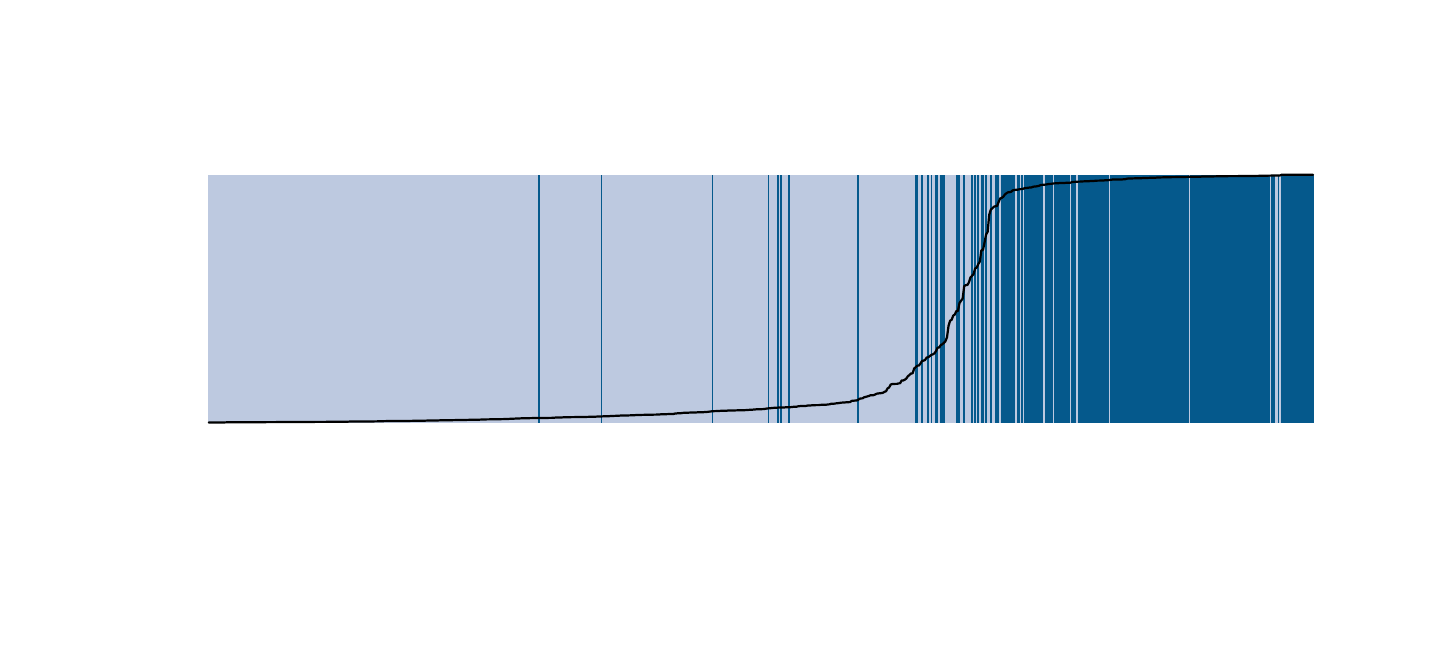
\begin{tikzpicture}[x=1pt,y=1pt]
\definecolor[named]{drawColor}{rgb}{0.00,0.00,0.00}
\definecolor[named]{fillColor}{rgb}{1.00,1.00,1.00}
\fill[color=fillColor,fill opacity=0.00,] (0,0) rectangle (505.89,216.81);
\begin{scope}
\path[clip] (  0.00,  0.00) rectangle (505.89,216.81);
\end{scope}
\begin{scope}
\path[clip] ( 49.20, 61.20) rectangle (480.69,167.61);
\definecolor[named]{fillColor}{rgb}{0.74,0.79,0.88}

\draw[fill=fillColor,draw opacity=0.00,] ( 65.18, 74.10) rectangle ( 65.75,163.67);

\draw[fill=fillColor,draw opacity=0.00,] ( 65.75, 74.10) rectangle ( 66.31,163.67);

\draw[fill=fillColor,draw opacity=0.00,] ( 66.31, 74.10) rectangle ( 66.88,163.67);

\draw[fill=fillColor,draw opacity=0.00,] ( 66.88, 74.10) rectangle ( 67.44,163.67);

\draw[fill=fillColor,draw opacity=0.00,] ( 67.44, 74.10) rectangle ( 68.01,163.67);

\draw[fill=fillColor,draw opacity=0.00,] ( 68.01, 74.10) rectangle ( 68.57,163.67);

\draw[fill=fillColor,draw opacity=0.00,] ( 68.57, 74.10) rectangle ( 69.14,163.67);

\draw[fill=fillColor,draw opacity=0.00,] ( 69.14, 74.10) rectangle ( 69.70,163.67);

\draw[fill=fillColor,draw opacity=0.00,] ( 69.70, 74.10) rectangle ( 70.27,163.67);

\draw[fill=fillColor,draw opacity=0.00,] ( 70.27, 74.10) rectangle ( 70.83,163.67);

\draw[fill=fillColor,draw opacity=0.00,] ( 70.83, 74.10) rectangle ( 71.40,163.67);

\draw[fill=fillColor,draw opacity=0.00,] ( 71.40, 74.10) rectangle ( 71.96,163.67);

\draw[fill=fillColor,draw opacity=0.00,] ( 71.96, 74.10) rectangle ( 72.53,163.67);

\draw[fill=fillColor,draw opacity=0.00,] ( 72.53, 74.10) rectangle ( 73.09,163.67);

\draw[fill=fillColor,draw opacity=0.00,] ( 73.09, 74.10) rectangle ( 73.66,163.67);

\draw[fill=fillColor,draw opacity=0.00,] ( 73.66, 74.10) rectangle ( 74.22,163.67);

\draw[fill=fillColor,draw opacity=0.00,] ( 74.22, 74.10) rectangle ( 74.79,163.67);

\draw[fill=fillColor,draw opacity=0.00,] ( 74.79, 74.10) rectangle ( 75.35,163.67);

\draw[fill=fillColor,draw opacity=0.00,] ( 75.35, 74.10) rectangle ( 75.92,163.67);

\draw[fill=fillColor,draw opacity=0.00,] ( 75.92, 74.10) rectangle ( 76.48,163.67);

\draw[fill=fillColor,draw opacity=0.00,] ( 76.48, 74.10) rectangle ( 77.05,163.67);

\draw[fill=fillColor,draw opacity=0.00,] ( 77.05, 74.10) rectangle ( 77.61,163.67);

\draw[fill=fillColor,draw opacity=0.00,] ( 77.61, 74.10) rectangle ( 78.18,163.67);

\draw[fill=fillColor,draw opacity=0.00,] ( 78.18, 74.10) rectangle ( 78.74,163.67);

\draw[fill=fillColor,draw opacity=0.00,] ( 78.74, 74.10) rectangle ( 79.31,163.67);

\draw[fill=fillColor,draw opacity=0.00,] ( 79.31, 74.10) rectangle ( 79.87,163.67);

\draw[fill=fillColor,draw opacity=0.00,] ( 79.87, 74.10) rectangle ( 80.44,163.67);

\draw[fill=fillColor,draw opacity=0.00,] ( 80.44, 74.10) rectangle ( 81.00,163.67);

\draw[fill=fillColor,draw opacity=0.00,] ( 81.00, 74.10) rectangle ( 81.57,163.67);

\draw[fill=fillColor,draw opacity=0.00,] ( 81.57, 74.10) rectangle ( 82.13,163.67);

\draw[fill=fillColor,draw opacity=0.00,] ( 82.13, 74.10) rectangle ( 82.70,163.67);

\draw[fill=fillColor,draw opacity=0.00,] ( 82.70, 74.10) rectangle ( 83.26,163.67);

\draw[fill=fillColor,draw opacity=0.00,] ( 83.26, 74.10) rectangle ( 83.83,163.67);

\draw[fill=fillColor,draw opacity=0.00,] ( 83.83, 74.10) rectangle ( 84.39,163.67);

\draw[fill=fillColor,draw opacity=0.00,] ( 84.39, 74.10) rectangle ( 84.96,163.67);

\draw[fill=fillColor,draw opacity=0.00,] ( 84.96, 74.10) rectangle ( 85.52,163.67);

\draw[fill=fillColor,draw opacity=0.00,] ( 85.52, 74.10) rectangle ( 86.09,163.67);

\draw[fill=fillColor,draw opacity=0.00,] ( 86.09, 74.10) rectangle ( 86.66,163.67);

\draw[fill=fillColor,draw opacity=0.00,] ( 86.66, 74.10) rectangle ( 87.22,163.67);

\draw[fill=fillColor,draw opacity=0.00,] ( 87.22, 74.10) rectangle ( 87.79,163.67);

\draw[fill=fillColor,draw opacity=0.00,] ( 87.79, 74.10) rectangle ( 88.35,163.67);

\draw[fill=fillColor,draw opacity=0.00,] ( 88.35, 74.10) rectangle ( 88.92,163.67);

\draw[fill=fillColor,draw opacity=0.00,] ( 88.92, 74.10) rectangle ( 89.48,163.67);

\draw[fill=fillColor,draw opacity=0.00,] ( 89.48, 74.10) rectangle ( 90.05,163.67);

\draw[fill=fillColor,draw opacity=0.00,] ( 90.05, 74.10) rectangle ( 90.61,163.67);

\draw[fill=fillColor,draw opacity=0.00,] ( 90.61, 74.10) rectangle ( 91.18,163.67);

\draw[fill=fillColor,draw opacity=0.00,] ( 91.18, 74.10) rectangle ( 91.74,163.67);

\draw[fill=fillColor,draw opacity=0.00,] ( 91.74, 74.10) rectangle ( 92.31,163.67);

\draw[fill=fillColor,draw opacity=0.00,] ( 92.31, 74.10) rectangle ( 92.87,163.67);

\draw[fill=fillColor,draw opacity=0.00,] ( 92.87, 74.10) rectangle ( 93.44,163.67);

\draw[fill=fillColor,draw opacity=0.00,] ( 93.44, 74.10) rectangle ( 94.00,163.67);

\draw[fill=fillColor,draw opacity=0.00,] ( 94.00, 74.10) rectangle ( 94.57,163.67);

\draw[fill=fillColor,draw opacity=0.00,] ( 94.57, 74.10) rectangle ( 95.13,163.67);

\draw[fill=fillColor,draw opacity=0.00,] ( 95.13, 74.10) rectangle ( 95.70,163.67);

\draw[fill=fillColor,draw opacity=0.00,] ( 95.70, 74.10) rectangle ( 96.26,163.67);

\draw[fill=fillColor,draw opacity=0.00,] ( 96.26, 74.10) rectangle ( 96.83,163.67);

\draw[fill=fillColor,draw opacity=0.00,] ( 96.83, 74.10) rectangle ( 97.39,163.67);

\draw[fill=fillColor,draw opacity=0.00,] ( 97.39, 74.10) rectangle ( 97.96,163.67);

\draw[fill=fillColor,draw opacity=0.00,] ( 97.96, 74.10) rectangle ( 98.52,163.67);

\draw[fill=fillColor,draw opacity=0.00,] ( 98.52, 74.10) rectangle ( 99.09,163.67);

\draw[fill=fillColor,draw opacity=0.00,] ( 99.09, 74.10) rectangle ( 99.65,163.67);

\draw[fill=fillColor,draw opacity=0.00,] ( 99.65, 74.10) rectangle (100.22,163.67);

\draw[fill=fillColor,draw opacity=0.00,] (100.22, 74.10) rectangle (100.78,163.67);

\draw[fill=fillColor,draw opacity=0.00,] (100.78, 74.10) rectangle (101.35,163.67);

\draw[fill=fillColor,draw opacity=0.00,] (101.35, 74.10) rectangle (101.91,163.67);

\draw[fill=fillColor,draw opacity=0.00,] (101.91, 74.10) rectangle (102.48,163.67);

\draw[fill=fillColor,draw opacity=0.00,] (102.48, 74.10) rectangle (103.04,163.67);

\draw[fill=fillColor,draw opacity=0.00,] (103.04, 74.10) rectangle (103.61,163.67);

\draw[fill=fillColor,draw opacity=0.00,] (103.61, 74.10) rectangle (104.17,163.67);

\draw[fill=fillColor,draw opacity=0.00,] (104.17, 74.10) rectangle (104.74,163.67);

\draw[fill=fillColor,draw opacity=0.00,] (104.74, 74.10) rectangle (105.30,163.67);

\draw[fill=fillColor,draw opacity=0.00,] (105.30, 74.10) rectangle (105.87,163.67);

\draw[fill=fillColor,draw opacity=0.00,] (105.87, 74.10) rectangle (106.43,163.67);

\draw[fill=fillColor,draw opacity=0.00,] (106.43, 74.10) rectangle (107.00,163.67);

\draw[fill=fillColor,draw opacity=0.00,] (107.00, 74.10) rectangle (107.56,163.67);

\draw[fill=fillColor,draw opacity=0.00,] (107.56, 74.10) rectangle (108.13,163.67);

\draw[fill=fillColor,draw opacity=0.00,] (108.13, 74.10) rectangle (108.69,163.67);

\draw[fill=fillColor,draw opacity=0.00,] (108.69, 74.10) rectangle (109.26,163.67);

\draw[fill=fillColor,draw opacity=0.00,] (109.26, 74.10) rectangle (109.82,163.67);

\draw[fill=fillColor,draw opacity=0.00,] (109.82, 74.10) rectangle (110.39,163.67);

\draw[fill=fillColor,draw opacity=0.00,] (110.39, 74.10) rectangle (110.95,163.67);

\draw[fill=fillColor,draw opacity=0.00,] (110.95, 74.10) rectangle (111.52,163.67);

\draw[fill=fillColor,draw opacity=0.00,] (111.52, 74.10) rectangle (112.08,163.67);

\draw[fill=fillColor,draw opacity=0.00,] (112.08, 74.10) rectangle (112.65,163.67);

\draw[fill=fillColor,draw opacity=0.00,] (112.65, 74.10) rectangle (113.21,163.67);

\draw[fill=fillColor,draw opacity=0.00,] (113.21, 74.10) rectangle (113.78,163.67);

\draw[fill=fillColor,draw opacity=0.00,] (113.78, 74.10) rectangle (114.35,163.67);

\draw[fill=fillColor,draw opacity=0.00,] (114.35, 74.10) rectangle (114.91,163.67);

\draw[fill=fillColor,draw opacity=0.00,] (114.91, 74.10) rectangle (115.48,163.67);

\draw[fill=fillColor,draw opacity=0.00,] (115.48, 74.10) rectangle (116.04,163.67);

\draw[fill=fillColor,draw opacity=0.00,] (116.04, 74.10) rectangle (116.61,163.67);

\draw[fill=fillColor,draw opacity=0.00,] (116.61, 74.10) rectangle (117.17,163.67);

\draw[fill=fillColor,draw opacity=0.00,] (117.17, 74.10) rectangle (117.74,163.67);

\draw[fill=fillColor,draw opacity=0.00,] (117.74, 74.10) rectangle (118.30,163.67);

\draw[fill=fillColor,draw opacity=0.00,] (118.30, 74.10) rectangle (118.87,163.67);

\draw[fill=fillColor,draw opacity=0.00,] (118.87, 74.10) rectangle (119.43,163.67);

\draw[fill=fillColor,draw opacity=0.00,] (119.43, 74.10) rectangle (120.00,163.67);

\draw[fill=fillColor,draw opacity=0.00,] (120.00, 74.10) rectangle (120.56,163.67);

\draw[fill=fillColor,draw opacity=0.00,] (120.56, 74.10) rectangle (121.13,163.67);

\draw[fill=fillColor,draw opacity=0.00,] (121.13, 74.10) rectangle (121.69,163.67);

\draw[fill=fillColor,draw opacity=0.00,] (121.69, 74.10) rectangle (122.26,163.67);

\draw[fill=fillColor,draw opacity=0.00,] (122.26, 74.10) rectangle (122.82,163.67);

\draw[fill=fillColor,draw opacity=0.00,] (122.82, 74.10) rectangle (123.39,163.67);

\draw[fill=fillColor,draw opacity=0.00,] (123.39, 74.10) rectangle (123.95,163.67);

\draw[fill=fillColor,draw opacity=0.00,] (123.95, 74.10) rectangle (124.52,163.67);

\draw[fill=fillColor,draw opacity=0.00,] (124.52, 74.10) rectangle (125.08,163.67);

\draw[fill=fillColor,draw opacity=0.00,] (125.08, 74.10) rectangle (125.65,163.67);

\draw[fill=fillColor,draw opacity=0.00,] (125.65, 74.10) rectangle (126.21,163.67);

\draw[fill=fillColor,draw opacity=0.00,] (126.21, 74.10) rectangle (126.78,163.67);

\draw[fill=fillColor,draw opacity=0.00,] (126.78, 74.10) rectangle (127.34,163.67);

\draw[fill=fillColor,draw opacity=0.00,] (127.34, 74.10) rectangle (127.91,163.67);

\draw[fill=fillColor,draw opacity=0.00,] (127.91, 74.10) rectangle (128.47,163.67);

\draw[fill=fillColor,draw opacity=0.00,] (128.47, 74.10) rectangle (129.04,163.67);

\draw[fill=fillColor,draw opacity=0.00,] (129.04, 74.10) rectangle (129.60,163.67);

\draw[fill=fillColor,draw opacity=0.00,] (129.60, 74.10) rectangle (130.17,163.67);

\draw[fill=fillColor,draw opacity=0.00,] (130.17, 74.10) rectangle (130.73,163.67);

\draw[fill=fillColor,draw opacity=0.00,] (130.73, 74.10) rectangle (131.30,163.67);

\draw[fill=fillColor,draw opacity=0.00,] (131.30, 74.10) rectangle (131.86,163.67);

\draw[fill=fillColor,draw opacity=0.00,] (131.86, 74.10) rectangle (132.43,163.67);

\draw[fill=fillColor,draw opacity=0.00,] (132.43, 74.10) rectangle (132.99,163.67);

\draw[fill=fillColor,draw opacity=0.00,] (132.99, 74.10) rectangle (133.56,163.67);

\draw[fill=fillColor,draw opacity=0.00,] (133.56, 74.10) rectangle (134.12,163.67);

\draw[fill=fillColor,draw opacity=0.00,] (134.12, 74.10) rectangle (134.69,163.67);

\draw[fill=fillColor,draw opacity=0.00,] (134.69, 74.10) rectangle (135.25,163.67);

\draw[fill=fillColor,draw opacity=0.00,] (135.25, 74.10) rectangle (135.82,163.67);

\draw[fill=fillColor,draw opacity=0.00,] (135.82, 74.10) rectangle (136.38,163.67);

\draw[fill=fillColor,draw opacity=0.00,] (136.38, 74.10) rectangle (136.95,163.67);

\draw[fill=fillColor,draw opacity=0.00,] (136.95, 74.10) rectangle (137.51,163.67);

\draw[fill=fillColor,draw opacity=0.00,] (137.51, 74.10) rectangle (138.08,163.67);

\draw[fill=fillColor,draw opacity=0.00,] (138.08, 74.10) rectangle (138.64,163.67);

\draw[fill=fillColor,draw opacity=0.00,] (138.64, 74.10) rectangle (139.21,163.67);

\draw[fill=fillColor,draw opacity=0.00,] (139.21, 74.10) rectangle (139.77,163.67);

\draw[fill=fillColor,draw opacity=0.00,] (139.77, 74.10) rectangle (140.34,163.67);

\draw[fill=fillColor,draw opacity=0.00,] (140.34, 74.10) rectangle (140.90,163.67);

\draw[fill=fillColor,draw opacity=0.00,] (140.90, 74.10) rectangle (141.47,163.67);

\draw[fill=fillColor,draw opacity=0.00,] (141.47, 74.10) rectangle (142.04,163.67);

\draw[fill=fillColor,draw opacity=0.00,] (142.04, 74.10) rectangle (142.60,163.67);

\draw[fill=fillColor,draw opacity=0.00,] (142.60, 74.10) rectangle (143.17,163.67);

\draw[fill=fillColor,draw opacity=0.00,] (143.17, 74.10) rectangle (143.73,163.67);

\draw[fill=fillColor,draw opacity=0.00,] (143.73, 74.10) rectangle (144.30,163.67);

\draw[fill=fillColor,draw opacity=0.00,] (144.30, 74.10) rectangle (144.86,163.67);

\draw[fill=fillColor,draw opacity=0.00,] (144.86, 74.10) rectangle (145.43,163.67);

\draw[fill=fillColor,draw opacity=0.00,] (145.43, 74.10) rectangle (145.99,163.67);

\draw[fill=fillColor,draw opacity=0.00,] (145.99, 74.10) rectangle (146.56,163.67);

\draw[fill=fillColor,draw opacity=0.00,] (146.56, 74.10) rectangle (147.12,163.67);

\draw[fill=fillColor,draw opacity=0.00,] (147.12, 74.10) rectangle (147.69,163.67);

\draw[fill=fillColor,draw opacity=0.00,] (147.69, 74.10) rectangle (148.25,163.67);

\draw[fill=fillColor,draw opacity=0.00,] (148.25, 74.10) rectangle (148.82,163.67);

\draw[fill=fillColor,draw opacity=0.00,] (148.82, 74.10) rectangle (149.38,163.67);

\draw[fill=fillColor,draw opacity=0.00,] (149.38, 74.10) rectangle (149.95,163.67);

\draw[fill=fillColor,draw opacity=0.00,] (149.95, 74.10) rectangle (150.51,163.67);

\draw[fill=fillColor,draw opacity=0.00,] (150.51, 74.10) rectangle (151.08,163.67);

\draw[fill=fillColor,draw opacity=0.00,] (151.08, 74.10) rectangle (151.64,163.67);

\draw[fill=fillColor,draw opacity=0.00,] (151.64, 74.10) rectangle (152.21,163.67);

\draw[fill=fillColor,draw opacity=0.00,] (152.21, 74.10) rectangle (152.77,163.67);

\draw[fill=fillColor,draw opacity=0.00,] (152.77, 74.10) rectangle (153.34,163.67);

\draw[fill=fillColor,draw opacity=0.00,] (153.34, 74.10) rectangle (153.90,163.67);

\draw[fill=fillColor,draw opacity=0.00,] (153.90, 74.10) rectangle (154.47,163.67);

\draw[fill=fillColor,draw opacity=0.00,] (154.47, 74.10) rectangle (155.03,163.67);

\draw[fill=fillColor,draw opacity=0.00,] (155.03, 74.10) rectangle (155.60,163.67);

\draw[fill=fillColor,draw opacity=0.00,] (155.60, 74.10) rectangle (156.16,163.67);

\draw[fill=fillColor,draw opacity=0.00,] (156.16, 74.10) rectangle (156.73,163.67);

\draw[fill=fillColor,draw opacity=0.00,] (156.73, 74.10) rectangle (157.29,163.67);

\draw[fill=fillColor,draw opacity=0.00,] (157.29, 74.10) rectangle (157.86,163.67);

\draw[fill=fillColor,draw opacity=0.00,] (157.86, 74.10) rectangle (158.42,163.67);

\draw[fill=fillColor,draw opacity=0.00,] (158.42, 74.10) rectangle (158.99,163.67);

\draw[fill=fillColor,draw opacity=0.00,] (158.99, 74.10) rectangle (159.55,163.67);

\draw[fill=fillColor,draw opacity=0.00,] (159.55, 74.10) rectangle (160.12,163.67);

\draw[fill=fillColor,draw opacity=0.00,] (160.12, 74.10) rectangle (160.68,163.67);

\draw[fill=fillColor,draw opacity=0.00,] (160.68, 74.10) rectangle (161.25,163.67);

\draw[fill=fillColor,draw opacity=0.00,] (161.25, 74.10) rectangle (161.81,163.67);

\draw[fill=fillColor,draw opacity=0.00,] (161.81, 74.10) rectangle (162.38,163.67);

\draw[fill=fillColor,draw opacity=0.00,] (162.38, 74.10) rectangle (162.94,163.67);

\draw[fill=fillColor,draw opacity=0.00,] (162.94, 74.10) rectangle (163.51,163.67);

\draw[fill=fillColor,draw opacity=0.00,] (163.51, 74.10) rectangle (164.07,163.67);

\draw[fill=fillColor,draw opacity=0.00,] (164.07, 74.10) rectangle (164.64,163.67);

\draw[fill=fillColor,draw opacity=0.00,] (164.64, 74.10) rectangle (165.20,163.67);

\draw[fill=fillColor,draw opacity=0.00,] (165.20, 74.10) rectangle (165.77,163.67);

\draw[fill=fillColor,draw opacity=0.00,] (165.77, 74.10) rectangle (166.33,163.67);

\draw[fill=fillColor,draw opacity=0.00,] (166.33, 74.10) rectangle (166.90,163.67);

\draw[fill=fillColor,draw opacity=0.00,] (166.90, 74.10) rectangle (167.46,163.67);

\draw[fill=fillColor,draw opacity=0.00,] (167.46, 74.10) rectangle (168.03,163.67);

\draw[fill=fillColor,draw opacity=0.00,] (168.03, 74.10) rectangle (168.59,163.67);

\draw[fill=fillColor,draw opacity=0.00,] (168.59, 74.10) rectangle (169.16,163.67);

\draw[fill=fillColor,draw opacity=0.00,] (169.16, 74.10) rectangle (169.73,163.67);

\draw[fill=fillColor,draw opacity=0.00,] (169.73, 74.10) rectangle (170.29,163.67);

\draw[fill=fillColor,draw opacity=0.00,] (170.29, 74.10) rectangle (170.86,163.67);

\draw[fill=fillColor,draw opacity=0.00,] (170.86, 74.10) rectangle (171.42,163.67);

\draw[fill=fillColor,draw opacity=0.00,] (171.42, 74.10) rectangle (171.99,163.67);

\draw[fill=fillColor,draw opacity=0.00,] (171.99, 74.10) rectangle (172.55,163.67);

\draw[fill=fillColor,draw opacity=0.00,] (172.55, 74.10) rectangle (173.12,163.67);

\draw[fill=fillColor,draw opacity=0.00,] (173.12, 74.10) rectangle (173.68,163.67);

\draw[fill=fillColor,draw opacity=0.00,] (173.68, 74.10) rectangle (174.25,163.67);

\draw[fill=fillColor,draw opacity=0.00,] (174.25, 74.10) rectangle (174.81,163.67);

\draw[fill=fillColor,draw opacity=0.00,] (174.81, 74.10) rectangle (175.38,163.67);

\draw[fill=fillColor,draw opacity=0.00,] (175.38, 74.10) rectangle (175.94,163.67);

\draw[fill=fillColor,draw opacity=0.00,] (175.94, 74.10) rectangle (176.51,163.67);

\draw[fill=fillColor,draw opacity=0.00,] (176.51, 74.10) rectangle (177.07,163.67);

\draw[fill=fillColor,draw opacity=0.00,] (177.07, 74.10) rectangle (177.64,163.67);

\draw[fill=fillColor,draw opacity=0.00,] (177.64, 74.10) rectangle (178.20,163.67);

\draw[fill=fillColor,draw opacity=0.00,] (178.20, 74.10) rectangle (178.77,163.67);

\draw[fill=fillColor,draw opacity=0.00,] (178.77, 74.10) rectangle (179.33,163.67);

\draw[fill=fillColor,draw opacity=0.00,] (179.33, 74.10) rectangle (179.90,163.67);

\draw[fill=fillColor,draw opacity=0.00,] (179.90, 74.10) rectangle (180.46,163.67);

\draw[fill=fillColor,draw opacity=0.00,] (180.46, 74.10) rectangle (181.03,163.67);

\draw[fill=fillColor,draw opacity=0.00,] (181.03, 74.10) rectangle (181.59,163.67);

\draw[fill=fillColor,draw opacity=0.00,] (181.59, 74.10) rectangle (182.16,163.67);

\draw[fill=fillColor,draw opacity=0.00,] (182.16, 74.10) rectangle (182.72,163.67);

\draw[fill=fillColor,draw opacity=0.00,] (182.72, 74.10) rectangle (183.29,163.67);

\draw[fill=fillColor,draw opacity=0.00,] (183.29, 74.10) rectangle (183.85,163.67);

\draw[fill=fillColor,draw opacity=0.00,] (183.85, 74.10) rectangle (184.42,163.67);
\definecolor[named]{fillColor}{rgb}{0.02,0.35,0.55}

\draw[fill=fillColor,draw opacity=0.00,] (184.42, 74.10) rectangle (184.98,163.67);
\definecolor[named]{fillColor}{rgb}{0.74,0.79,0.88}

\draw[fill=fillColor,draw opacity=0.00,] (184.98, 74.10) rectangle (185.55,163.67);

\draw[fill=fillColor,draw opacity=0.00,] (185.55, 74.10) rectangle (186.11,163.67);

\draw[fill=fillColor,draw opacity=0.00,] (186.11, 74.10) rectangle (186.68,163.67);

\draw[fill=fillColor,draw opacity=0.00,] (186.68, 74.10) rectangle (187.24,163.67);

\draw[fill=fillColor,draw opacity=0.00,] (187.24, 74.10) rectangle (187.81,163.67);

\draw[fill=fillColor,draw opacity=0.00,] (187.81, 74.10) rectangle (188.37,163.67);

\draw[fill=fillColor,draw opacity=0.00,] (188.37, 74.10) rectangle (188.94,163.67);

\draw[fill=fillColor,draw opacity=0.00,] (188.94, 74.10) rectangle (189.50,163.67);

\draw[fill=fillColor,draw opacity=0.00,] (189.50, 74.10) rectangle (190.07,163.67);

\draw[fill=fillColor,draw opacity=0.00,] (190.07, 74.10) rectangle (190.63,163.67);

\draw[fill=fillColor,draw opacity=0.00,] (190.63, 74.10) rectangle (191.20,163.67);

\draw[fill=fillColor,draw opacity=0.00,] (191.20, 74.10) rectangle (191.76,163.67);

\draw[fill=fillColor,draw opacity=0.00,] (191.76, 74.10) rectangle (192.33,163.67);

\draw[fill=fillColor,draw opacity=0.00,] (192.33, 74.10) rectangle (192.89,163.67);

\draw[fill=fillColor,draw opacity=0.00,] (192.89, 74.10) rectangle (193.46,163.67);

\draw[fill=fillColor,draw opacity=0.00,] (193.46, 74.10) rectangle (194.02,163.67);

\draw[fill=fillColor,draw opacity=0.00,] (194.02, 74.10) rectangle (194.59,163.67);

\draw[fill=fillColor,draw opacity=0.00,] (194.59, 74.10) rectangle (195.15,163.67);

\draw[fill=fillColor,draw opacity=0.00,] (195.15, 74.10) rectangle (195.72,163.67);

\draw[fill=fillColor,draw opacity=0.00,] (195.72, 74.10) rectangle (196.28,163.67);

\draw[fill=fillColor,draw opacity=0.00,] (196.28, 74.10) rectangle (196.85,163.67);

\draw[fill=fillColor,draw opacity=0.00,] (196.85, 74.10) rectangle (197.42,163.67);

\draw[fill=fillColor,draw opacity=0.00,] (197.42, 74.10) rectangle (197.98,163.67);

\draw[fill=fillColor,draw opacity=0.00,] (197.98, 74.10) rectangle (198.55,163.67);

\draw[fill=fillColor,draw opacity=0.00,] (198.55, 74.10) rectangle (199.11,163.67);

\draw[fill=fillColor,draw opacity=0.00,] (199.11, 74.10) rectangle (199.68,163.67);

\draw[fill=fillColor,draw opacity=0.00,] (199.68, 74.10) rectangle (200.24,163.67);

\draw[fill=fillColor,draw opacity=0.00,] (200.24, 74.10) rectangle (200.81,163.67);

\draw[fill=fillColor,draw opacity=0.00,] (200.81, 74.10) rectangle (201.37,163.67);

\draw[fill=fillColor,draw opacity=0.00,] (201.37, 74.10) rectangle (201.94,163.67);

\draw[fill=fillColor,draw opacity=0.00,] (201.94, 74.10) rectangle (202.50,163.67);

\draw[fill=fillColor,draw opacity=0.00,] (202.50, 74.10) rectangle (203.07,163.67);

\draw[fill=fillColor,draw opacity=0.00,] (203.07, 74.10) rectangle (203.63,163.67);

\draw[fill=fillColor,draw opacity=0.00,] (203.63, 74.10) rectangle (204.20,163.67);

\draw[fill=fillColor,draw opacity=0.00,] (204.20, 74.10) rectangle (204.76,163.67);

\draw[fill=fillColor,draw opacity=0.00,] (204.76, 74.10) rectangle (205.33,163.67);

\draw[fill=fillColor,draw opacity=0.00,] (205.33, 74.10) rectangle (205.89,163.67);

\draw[fill=fillColor,draw opacity=0.00,] (205.89, 74.10) rectangle (206.46,163.67);

\draw[fill=fillColor,draw opacity=0.00,] (206.46, 74.10) rectangle (207.02,163.67);
\definecolor[named]{fillColor}{rgb}{0.02,0.35,0.55}

\draw[fill=fillColor,draw opacity=0.00,] (207.02, 74.10) rectangle (207.59,163.67);
\definecolor[named]{fillColor}{rgb}{0.74,0.79,0.88}

\draw[fill=fillColor,draw opacity=0.00,] (207.59, 74.10) rectangle (208.15,163.67);

\draw[fill=fillColor,draw opacity=0.00,] (208.15, 74.10) rectangle (208.72,163.67);

\draw[fill=fillColor,draw opacity=0.00,] (208.72, 74.10) rectangle (209.28,163.67);

\draw[fill=fillColor,draw opacity=0.00,] (209.28, 74.10) rectangle (209.85,163.67);

\draw[fill=fillColor,draw opacity=0.00,] (209.85, 74.10) rectangle (210.41,163.67);

\draw[fill=fillColor,draw opacity=0.00,] (210.41, 74.10) rectangle (210.98,163.67);

\draw[fill=fillColor,draw opacity=0.00,] (210.98, 74.10) rectangle (211.54,163.67);

\draw[fill=fillColor,draw opacity=0.00,] (211.54, 74.10) rectangle (212.11,163.67);

\draw[fill=fillColor,draw opacity=0.00,] (212.11, 74.10) rectangle (212.67,163.67);

\draw[fill=fillColor,draw opacity=0.00,] (212.67, 74.10) rectangle (213.24,163.67);

\draw[fill=fillColor,draw opacity=0.00,] (213.24, 74.10) rectangle (213.80,163.67);

\draw[fill=fillColor,draw opacity=0.00,] (213.80, 74.10) rectangle (214.37,163.67);

\draw[fill=fillColor,draw opacity=0.00,] (214.37, 74.10) rectangle (214.93,163.67);

\draw[fill=fillColor,draw opacity=0.00,] (214.93, 74.10) rectangle (215.50,163.67);

\draw[fill=fillColor,draw opacity=0.00,] (215.50, 74.10) rectangle (216.06,163.67);

\draw[fill=fillColor,draw opacity=0.00,] (216.06, 74.10) rectangle (216.63,163.67);

\draw[fill=fillColor,draw opacity=0.00,] (216.63, 74.10) rectangle (217.19,163.67);

\draw[fill=fillColor,draw opacity=0.00,] (217.19, 74.10) rectangle (217.76,163.67);

\draw[fill=fillColor,draw opacity=0.00,] (217.76, 74.10) rectangle (218.32,163.67);

\draw[fill=fillColor,draw opacity=0.00,] (218.32, 74.10) rectangle (218.89,163.67);

\draw[fill=fillColor,draw opacity=0.00,] (218.89, 74.10) rectangle (219.45,163.67);

\draw[fill=fillColor,draw opacity=0.00,] (219.45, 74.10) rectangle (220.02,163.67);

\draw[fill=fillColor,draw opacity=0.00,] (220.02, 74.10) rectangle (220.58,163.67);

\draw[fill=fillColor,draw opacity=0.00,] (220.58, 74.10) rectangle (221.15,163.67);

\draw[fill=fillColor,draw opacity=0.00,] (221.15, 74.10) rectangle (221.71,163.67);

\draw[fill=fillColor,draw opacity=0.00,] (221.71, 74.10) rectangle (222.28,163.67);

\draw[fill=fillColor,draw opacity=0.00,] (222.28, 74.10) rectangle (222.84,163.67);

\draw[fill=fillColor,draw opacity=0.00,] (222.84, 74.10) rectangle (223.41,163.67);

\draw[fill=fillColor,draw opacity=0.00,] (223.41, 74.10) rectangle (223.98,163.67);

\draw[fill=fillColor,draw opacity=0.00,] (223.98, 74.10) rectangle (224.54,163.67);

\draw[fill=fillColor,draw opacity=0.00,] (224.54, 74.10) rectangle (225.11,163.67);

\draw[fill=fillColor,draw opacity=0.00,] (225.11, 74.10) rectangle (225.67,163.67);

\draw[fill=fillColor,draw opacity=0.00,] (225.67, 74.10) rectangle (226.24,163.67);

\draw[fill=fillColor,draw opacity=0.00,] (226.24, 74.10) rectangle (226.80,163.67);

\draw[fill=fillColor,draw opacity=0.00,] (226.80, 74.10) rectangle (227.37,163.67);

\draw[fill=fillColor,draw opacity=0.00,] (227.37, 74.10) rectangle (227.93,163.67);

\draw[fill=fillColor,draw opacity=0.00,] (227.93, 74.10) rectangle (228.50,163.67);

\draw[fill=fillColor,draw opacity=0.00,] (228.50, 74.10) rectangle (229.06,163.67);

\draw[fill=fillColor,draw opacity=0.00,] (229.06, 74.10) rectangle (229.63,163.67);

\draw[fill=fillColor,draw opacity=0.00,] (229.63, 74.10) rectangle (230.19,163.67);

\draw[fill=fillColor,draw opacity=0.00,] (230.19, 74.10) rectangle (230.76,163.67);

\draw[fill=fillColor,draw opacity=0.00,] (230.76, 74.10) rectangle (231.32,163.67);

\draw[fill=fillColor,draw opacity=0.00,] (231.32, 74.10) rectangle (231.89,163.67);

\draw[fill=fillColor,draw opacity=0.00,] (231.89, 74.10) rectangle (232.45,163.67);

\draw[fill=fillColor,draw opacity=0.00,] (232.45, 74.10) rectangle (233.02,163.67);

\draw[fill=fillColor,draw opacity=0.00,] (233.02, 74.10) rectangle (233.58,163.67);

\draw[fill=fillColor,draw opacity=0.00,] (233.58, 74.10) rectangle (234.15,163.67);

\draw[fill=fillColor,draw opacity=0.00,] (234.15, 74.10) rectangle (234.71,163.67);

\draw[fill=fillColor,draw opacity=0.00,] (234.71, 74.10) rectangle (235.28,163.67);

\draw[fill=fillColor,draw opacity=0.00,] (235.28, 74.10) rectangle (235.84,163.67);

\draw[fill=fillColor,draw opacity=0.00,] (235.84, 74.10) rectangle (236.41,163.67);

\draw[fill=fillColor,draw opacity=0.00,] (236.41, 74.10) rectangle (236.97,163.67);

\draw[fill=fillColor,draw opacity=0.00,] (236.97, 74.10) rectangle (237.54,163.67);

\draw[fill=fillColor,draw opacity=0.00,] (237.54, 74.10) rectangle (238.10,163.67);

\draw[fill=fillColor,draw opacity=0.00,] (238.10, 74.10) rectangle (238.67,163.67);

\draw[fill=fillColor,draw opacity=0.00,] (238.67, 74.10) rectangle (239.23,163.67);

\draw[fill=fillColor,draw opacity=0.00,] (239.23, 74.10) rectangle (239.80,163.67);

\draw[fill=fillColor,draw opacity=0.00,] (239.80, 74.10) rectangle (240.36,163.67);

\draw[fill=fillColor,draw opacity=0.00,] (240.36, 74.10) rectangle (240.93,163.67);

\draw[fill=fillColor,draw opacity=0.00,] (240.93, 74.10) rectangle (241.49,163.67);

\draw[fill=fillColor,draw opacity=0.00,] (241.49, 74.10) rectangle (242.06,163.67);

\draw[fill=fillColor,draw opacity=0.00,] (242.06, 74.10) rectangle (242.62,163.67);

\draw[fill=fillColor,draw opacity=0.00,] (242.62, 74.10) rectangle (243.19,163.67);

\draw[fill=fillColor,draw opacity=0.00,] (243.19, 74.10) rectangle (243.75,163.67);

\draw[fill=fillColor,draw opacity=0.00,] (243.75, 74.10) rectangle (244.32,163.67);

\draw[fill=fillColor,draw opacity=0.00,] (244.32, 74.10) rectangle (244.88,163.67);

\draw[fill=fillColor,draw opacity=0.00,] (244.88, 74.10) rectangle (245.45,163.67);

\draw[fill=fillColor,draw opacity=0.00,] (245.45, 74.10) rectangle (246.01,163.67);

\draw[fill=fillColor,draw opacity=0.00,] (246.01, 74.10) rectangle (246.58,163.67);

\draw[fill=fillColor,draw opacity=0.00,] (246.58, 74.10) rectangle (247.14,163.67);
\definecolor[named]{fillColor}{rgb}{0.02,0.35,0.55}

\draw[fill=fillColor,draw opacity=0.00,] (247.14, 74.10) rectangle (247.71,163.67);
\definecolor[named]{fillColor}{rgb}{0.74,0.79,0.88}

\draw[fill=fillColor,draw opacity=0.00,] (247.71, 74.10) rectangle (248.27,163.67);

\draw[fill=fillColor,draw opacity=0.00,] (248.27, 74.10) rectangle (248.84,163.67);

\draw[fill=fillColor,draw opacity=0.00,] (248.84, 74.10) rectangle (249.40,163.67);

\draw[fill=fillColor,draw opacity=0.00,] (249.40, 74.10) rectangle (249.97,163.67);

\draw[fill=fillColor,draw opacity=0.00,] (249.97, 74.10) rectangle (250.53,163.67);

\draw[fill=fillColor,draw opacity=0.00,] (250.53, 74.10) rectangle (251.10,163.67);

\draw[fill=fillColor,draw opacity=0.00,] (251.10, 74.10) rectangle (251.67,163.67);

\draw[fill=fillColor,draw opacity=0.00,] (251.67, 74.10) rectangle (252.23,163.67);

\draw[fill=fillColor,draw opacity=0.00,] (252.23, 74.10) rectangle (252.80,163.67);

\draw[fill=fillColor,draw opacity=0.00,] (252.80, 74.10) rectangle (253.36,163.67);

\draw[fill=fillColor,draw opacity=0.00,] (253.36, 74.10) rectangle (253.93,163.67);

\draw[fill=fillColor,draw opacity=0.00,] (253.93, 74.10) rectangle (254.49,163.67);

\draw[fill=fillColor,draw opacity=0.00,] (254.49, 74.10) rectangle (255.06,163.67);

\draw[fill=fillColor,draw opacity=0.00,] (255.06, 74.10) rectangle (255.62,163.67);

\draw[fill=fillColor,draw opacity=0.00,] (255.62, 74.10) rectangle (256.19,163.67);

\draw[fill=fillColor,draw opacity=0.00,] (256.19, 74.10) rectangle (256.75,163.67);

\draw[fill=fillColor,draw opacity=0.00,] (256.75, 74.10) rectangle (257.32,163.67);

\draw[fill=fillColor,draw opacity=0.00,] (257.32, 74.10) rectangle (257.88,163.67);

\draw[fill=fillColor,draw opacity=0.00,] (257.88, 74.10) rectangle (258.45,163.67);

\draw[fill=fillColor,draw opacity=0.00,] (258.45, 74.10) rectangle (259.01,163.67);

\draw[fill=fillColor,draw opacity=0.00,] (259.01, 74.10) rectangle (259.58,163.67);

\draw[fill=fillColor,draw opacity=0.00,] (259.58, 74.10) rectangle (260.14,163.67);

\draw[fill=fillColor,draw opacity=0.00,] (260.14, 74.10) rectangle (260.71,163.67);

\draw[fill=fillColor,draw opacity=0.00,] (260.71, 74.10) rectangle (261.27,163.67);

\draw[fill=fillColor,draw opacity=0.00,] (261.27, 74.10) rectangle (261.84,163.67);

\draw[fill=fillColor,draw opacity=0.00,] (261.84, 74.10) rectangle (262.40,163.67);

\draw[fill=fillColor,draw opacity=0.00,] (262.40, 74.10) rectangle (262.97,163.67);

\draw[fill=fillColor,draw opacity=0.00,] (262.97, 74.10) rectangle (263.53,163.67);

\draw[fill=fillColor,draw opacity=0.00,] (263.53, 74.10) rectangle (264.10,163.67);

\draw[fill=fillColor,draw opacity=0.00,] (264.10, 74.10) rectangle (264.66,163.67);

\draw[fill=fillColor,draw opacity=0.00,] (264.66, 74.10) rectangle (265.23,163.67);

\draw[fill=fillColor,draw opacity=0.00,] (265.23, 74.10) rectangle (265.79,163.67);

\draw[fill=fillColor,draw opacity=0.00,] (265.79, 74.10) rectangle (266.36,163.67);

\draw[fill=fillColor,draw opacity=0.00,] (266.36, 74.10) rectangle (266.92,163.67);

\draw[fill=fillColor,draw opacity=0.00,] (266.92, 74.10) rectangle (267.49,163.67);
\definecolor[named]{fillColor}{rgb}{0.02,0.35,0.55}

\draw[fill=fillColor,draw opacity=0.00,] (267.49, 74.10) rectangle (268.05,163.67);
\definecolor[named]{fillColor}{rgb}{0.74,0.79,0.88}

\draw[fill=fillColor,draw opacity=0.00,] (268.05, 74.10) rectangle (268.62,163.67);

\draw[fill=fillColor,draw opacity=0.00,] (268.62, 74.10) rectangle (269.18,163.67);

\draw[fill=fillColor,draw opacity=0.00,] (269.18, 74.10) rectangle (269.75,163.67);

\draw[fill=fillColor,draw opacity=0.00,] (269.75, 74.10) rectangle (270.31,163.67);

\draw[fill=fillColor,draw opacity=0.00,] (270.31, 74.10) rectangle (270.88,163.67);
\definecolor[named]{fillColor}{rgb}{0.02,0.35,0.55}

\draw[fill=fillColor,draw opacity=0.00,] (270.88, 74.10) rectangle (271.44,163.67);
\definecolor[named]{fillColor}{rgb}{0.74,0.79,0.88}

\draw[fill=fillColor,draw opacity=0.00,] (271.44, 74.10) rectangle (272.01,163.67);
\definecolor[named]{fillColor}{rgb}{0.02,0.35,0.55}

\draw[fill=fillColor,draw opacity=0.00,] (272.01, 74.10) rectangle (272.57,163.67);
\definecolor[named]{fillColor}{rgb}{0.74,0.79,0.88}

\draw[fill=fillColor,draw opacity=0.00,] (272.57, 74.10) rectangle (273.14,163.67);

\draw[fill=fillColor,draw opacity=0.00,] (273.14, 74.10) rectangle (273.70,163.67);

\draw[fill=fillColor,draw opacity=0.00,] (273.70, 74.10) rectangle (274.27,163.67);

\draw[fill=fillColor,draw opacity=0.00,] (274.27, 74.10) rectangle (274.83,163.67);
\definecolor[named]{fillColor}{rgb}{0.02,0.35,0.55}

\draw[fill=fillColor,draw opacity=0.00,] (274.83, 74.10) rectangle (275.40,163.67);
\definecolor[named]{fillColor}{rgb}{0.74,0.79,0.88}

\draw[fill=fillColor,draw opacity=0.00,] (275.40, 74.10) rectangle (275.96,163.67);

\draw[fill=fillColor,draw opacity=0.00,] (275.96, 74.10) rectangle (276.53,163.67);

\draw[fill=fillColor,draw opacity=0.00,] (276.53, 74.10) rectangle (277.09,163.67);

\draw[fill=fillColor,draw opacity=0.00,] (277.09, 74.10) rectangle (277.66,163.67);

\draw[fill=fillColor,draw opacity=0.00,] (277.66, 74.10) rectangle (278.22,163.67);

\draw[fill=fillColor,draw opacity=0.00,] (278.22, 74.10) rectangle (278.79,163.67);

\draw[fill=fillColor,draw opacity=0.00,] (278.79, 74.10) rectangle (279.36,163.67);

\draw[fill=fillColor,draw opacity=0.00,] (279.36, 74.10) rectangle (279.92,163.67);

\draw[fill=fillColor,draw opacity=0.00,] (279.92, 74.10) rectangle (280.49,163.67);

\draw[fill=fillColor,draw opacity=0.00,] (280.49, 74.10) rectangle (281.05,163.67);

\draw[fill=fillColor,draw opacity=0.00,] (281.05, 74.10) rectangle (281.62,163.67);

\draw[fill=fillColor,draw opacity=0.00,] (281.62, 74.10) rectangle (282.18,163.67);

\draw[fill=fillColor,draw opacity=0.00,] (282.18, 74.10) rectangle (282.75,163.67);

\draw[fill=fillColor,draw opacity=0.00,] (282.75, 74.10) rectangle (283.31,163.67);

\draw[fill=fillColor,draw opacity=0.00,] (283.31, 74.10) rectangle (283.88,163.67);

\draw[fill=fillColor,draw opacity=0.00,] (283.88, 74.10) rectangle (284.44,163.67);

\draw[fill=fillColor,draw opacity=0.00,] (284.44, 74.10) rectangle (285.01,163.67);

\draw[fill=fillColor,draw opacity=0.00,] (285.01, 74.10) rectangle (285.57,163.67);

\draw[fill=fillColor,draw opacity=0.00,] (285.57, 74.10) rectangle (286.14,163.67);

\draw[fill=fillColor,draw opacity=0.00,] (286.14, 74.10) rectangle (286.70,163.67);

\draw[fill=fillColor,draw opacity=0.00,] (286.70, 74.10) rectangle (287.27,163.67);

\draw[fill=fillColor,draw opacity=0.00,] (287.27, 74.10) rectangle (287.83,163.67);

\draw[fill=fillColor,draw opacity=0.00,] (287.83, 74.10) rectangle (288.40,163.67);

\draw[fill=fillColor,draw opacity=0.00,] (288.40, 74.10) rectangle (288.96,163.67);

\draw[fill=fillColor,draw opacity=0.00,] (288.96, 74.10) rectangle (289.53,163.67);

\draw[fill=fillColor,draw opacity=0.00,] (289.53, 74.10) rectangle (290.09,163.67);

\draw[fill=fillColor,draw opacity=0.00,] (290.09, 74.10) rectangle (290.66,163.67);

\draw[fill=fillColor,draw opacity=0.00,] (290.66, 74.10) rectangle (291.22,163.67);

\draw[fill=fillColor,draw opacity=0.00,] (291.22, 74.10) rectangle (291.79,163.67);

\draw[fill=fillColor,draw opacity=0.00,] (291.79, 74.10) rectangle (292.35,163.67);

\draw[fill=fillColor,draw opacity=0.00,] (292.35, 74.10) rectangle (292.92,163.67);

\draw[fill=fillColor,draw opacity=0.00,] (292.92, 74.10) rectangle (293.48,163.67);

\draw[fill=fillColor,draw opacity=0.00,] (293.48, 74.10) rectangle (294.05,163.67);

\draw[fill=fillColor,draw opacity=0.00,] (294.05, 74.10) rectangle (294.61,163.67);

\draw[fill=fillColor,draw opacity=0.00,] (294.61, 74.10) rectangle (295.18,163.67);

\draw[fill=fillColor,draw opacity=0.00,] (295.18, 74.10) rectangle (295.74,163.67);

\draw[fill=fillColor,draw opacity=0.00,] (295.74, 74.10) rectangle (296.31,163.67);

\draw[fill=fillColor,draw opacity=0.00,] (296.31, 74.10) rectangle (296.87,163.67);

\draw[fill=fillColor,draw opacity=0.00,] (296.87, 74.10) rectangle (297.44,163.67);

\draw[fill=fillColor,draw opacity=0.00,] (297.44, 74.10) rectangle (298.00,163.67);

\draw[fill=fillColor,draw opacity=0.00,] (298.00, 74.10) rectangle (298.57,163.67);

\draw[fill=fillColor,draw opacity=0.00,] (298.57, 74.10) rectangle (299.13,163.67);

\draw[fill=fillColor,draw opacity=0.00,] (299.13, 74.10) rectangle (299.70,163.67);
\definecolor[named]{fillColor}{rgb}{0.02,0.35,0.55}

\draw[fill=fillColor,draw opacity=0.00,] (299.70, 74.10) rectangle (300.26,163.67);
\definecolor[named]{fillColor}{rgb}{0.74,0.79,0.88}

\draw[fill=fillColor,draw opacity=0.00,] (300.26, 74.10) rectangle (300.83,163.67);

\draw[fill=fillColor,draw opacity=0.00,] (300.83, 74.10) rectangle (301.39,163.67);

\draw[fill=fillColor,draw opacity=0.00,] (301.39, 74.10) rectangle (301.96,163.67);

\draw[fill=fillColor,draw opacity=0.00,] (301.96, 74.10) rectangle (302.52,163.67);

\draw[fill=fillColor,draw opacity=0.00,] (302.52, 74.10) rectangle (303.09,163.67);

\draw[fill=fillColor,draw opacity=0.00,] (303.09, 74.10) rectangle (303.65,163.67);

\draw[fill=fillColor,draw opacity=0.00,] (303.65, 74.10) rectangle (304.22,163.67);

\draw[fill=fillColor,draw opacity=0.00,] (304.22, 74.10) rectangle (304.78,163.67);

\draw[fill=fillColor,draw opacity=0.00,] (304.78, 74.10) rectangle (305.35,163.67);

\draw[fill=fillColor,draw opacity=0.00,] (305.35, 74.10) rectangle (305.91,163.67);

\draw[fill=fillColor,draw opacity=0.00,] (305.91, 74.10) rectangle (306.48,163.67);

\draw[fill=fillColor,draw opacity=0.00,] (306.48, 74.10) rectangle (307.05,163.67);

\draw[fill=fillColor,draw opacity=0.00,] (307.05, 74.10) rectangle (307.61,163.67);

\draw[fill=fillColor,draw opacity=0.00,] (307.61, 74.10) rectangle (308.18,163.67);

\draw[fill=fillColor,draw opacity=0.00,] (308.18, 74.10) rectangle (308.74,163.67);

\draw[fill=fillColor,draw opacity=0.00,] (308.74, 74.10) rectangle (309.31,163.67);

\draw[fill=fillColor,draw opacity=0.00,] (309.31, 74.10) rectangle (309.87,163.67);

\draw[fill=fillColor,draw opacity=0.00,] (309.87, 74.10) rectangle (310.44,163.67);

\draw[fill=fillColor,draw opacity=0.00,] (310.44, 74.10) rectangle (311.00,163.67);

\draw[fill=fillColor,draw opacity=0.00,] (311.00, 74.10) rectangle (311.57,163.67);

\draw[fill=fillColor,draw opacity=0.00,] (311.57, 74.10) rectangle (312.13,163.67);

\draw[fill=fillColor,draw opacity=0.00,] (312.13, 74.10) rectangle (312.70,163.67);

\draw[fill=fillColor,draw opacity=0.00,] (312.70, 74.10) rectangle (313.26,163.67);

\draw[fill=fillColor,draw opacity=0.00,] (313.26, 74.10) rectangle (313.83,163.67);

\draw[fill=fillColor,draw opacity=0.00,] (313.83, 74.10) rectangle (314.39,163.67);

\draw[fill=fillColor,draw opacity=0.00,] (314.39, 74.10) rectangle (314.96,163.67);

\draw[fill=fillColor,draw opacity=0.00,] (314.96, 74.10) rectangle (315.52,163.67);

\draw[fill=fillColor,draw opacity=0.00,] (315.52, 74.10) rectangle (316.09,163.67);

\draw[fill=fillColor,draw opacity=0.00,] (316.09, 74.10) rectangle (316.65,163.67);

\draw[fill=fillColor,draw opacity=0.00,] (316.65, 74.10) rectangle (317.22,163.67);

\draw[fill=fillColor,draw opacity=0.00,] (317.22, 74.10) rectangle (317.78,163.67);

\draw[fill=fillColor,draw opacity=0.00,] (317.78, 74.10) rectangle (318.35,163.67);

\draw[fill=fillColor,draw opacity=0.00,] (318.35, 74.10) rectangle (318.91,163.67);

\draw[fill=fillColor,draw opacity=0.00,] (318.91, 74.10) rectangle (319.48,163.67);

\draw[fill=fillColor,draw opacity=0.00,] (319.48, 74.10) rectangle (320.04,163.67);

\draw[fill=fillColor,draw opacity=0.00,] (320.04, 74.10) rectangle (320.61,163.67);
\definecolor[named]{fillColor}{rgb}{0.02,0.35,0.55}

\draw[fill=fillColor,draw opacity=0.00,] (320.61, 74.10) rectangle (321.17,163.67);

\draw[fill=fillColor,draw opacity=0.00,] (321.17, 74.10) rectangle (321.74,163.67);
\definecolor[named]{fillColor}{rgb}{0.74,0.79,0.88}

\draw[fill=fillColor,draw opacity=0.00,] (321.74, 74.10) rectangle (322.30,163.67);

\draw[fill=fillColor,draw opacity=0.00,] (322.30, 74.10) rectangle (322.87,163.67);
\definecolor[named]{fillColor}{rgb}{0.02,0.35,0.55}

\draw[fill=fillColor,draw opacity=0.00,] (322.87, 74.10) rectangle (323.43,163.67);
\definecolor[named]{fillColor}{rgb}{0.74,0.79,0.88}

\draw[fill=fillColor,draw opacity=0.00,] (323.43, 74.10) rectangle (324.00,163.67);

\draw[fill=fillColor,draw opacity=0.00,] (324.00, 74.10) rectangle (324.56,163.67);

\draw[fill=fillColor,draw opacity=0.00,] (324.56, 74.10) rectangle (325.13,163.67);
\definecolor[named]{fillColor}{rgb}{0.02,0.35,0.55}

\draw[fill=fillColor,draw opacity=0.00,] (325.13, 74.10) rectangle (325.69,163.67);
\definecolor[named]{fillColor}{rgb}{0.74,0.79,0.88}

\draw[fill=fillColor,draw opacity=0.00,] (325.69, 74.10) rectangle (326.26,163.67);
\definecolor[named]{fillColor}{rgb}{0.02,0.35,0.55}

\draw[fill=fillColor,draw opacity=0.00,] (326.26, 74.10) rectangle (326.82,163.67);
\definecolor[named]{fillColor}{rgb}{0.74,0.79,0.88}

\draw[fill=fillColor,draw opacity=0.00,] (326.82, 74.10) rectangle (327.39,163.67);

\draw[fill=fillColor,draw opacity=0.00,] (327.39, 74.10) rectangle (327.95,163.67);
\definecolor[named]{fillColor}{rgb}{0.02,0.35,0.55}

\draw[fill=fillColor,draw opacity=0.00,] (327.95, 74.10) rectangle (328.52,163.67);

\draw[fill=fillColor,draw opacity=0.00,] (328.52, 74.10) rectangle (329.08,163.67);
\definecolor[named]{fillColor}{rgb}{0.74,0.79,0.88}

\draw[fill=fillColor,draw opacity=0.00,] (329.08, 74.10) rectangle (329.65,163.67);
\definecolor[named]{fillColor}{rgb}{0.02,0.35,0.55}

\draw[fill=fillColor,draw opacity=0.00,] (329.65, 74.10) rectangle (330.21,163.67);

\draw[fill=fillColor,draw opacity=0.00,] (330.21, 74.10) rectangle (330.78,163.67);

\draw[fill=fillColor,draw opacity=0.00,] (330.78, 74.10) rectangle (331.34,163.67);
\definecolor[named]{fillColor}{rgb}{0.74,0.79,0.88}

\draw[fill=fillColor,draw opacity=0.00,] (331.34, 74.10) rectangle (331.91,163.67);

\draw[fill=fillColor,draw opacity=0.00,] (331.91, 74.10) rectangle (332.47,163.67);

\draw[fill=fillColor,draw opacity=0.00,] (332.47, 74.10) rectangle (333.04,163.67);

\draw[fill=fillColor,draw opacity=0.00,] (333.04, 74.10) rectangle (333.61,163.67);

\draw[fill=fillColor,draw opacity=0.00,] (333.61, 74.10) rectangle (334.17,163.67);

\draw[fill=fillColor,draw opacity=0.00,] (334.17, 74.10) rectangle (334.74,163.67);

\draw[fill=fillColor,draw opacity=0.00,] (334.74, 74.10) rectangle (335.30,163.67);
\definecolor[named]{fillColor}{rgb}{0.02,0.35,0.55}

\draw[fill=fillColor,draw opacity=0.00,] (335.30, 74.10) rectangle (335.87,163.67);

\draw[fill=fillColor,draw opacity=0.00,] (335.87, 74.10) rectangle (336.43,163.67);

\draw[fill=fillColor,draw opacity=0.00,] (336.43, 74.10) rectangle (337.00,163.67);
\definecolor[named]{fillColor}{rgb}{0.74,0.79,0.88}

\draw[fill=fillColor,draw opacity=0.00,] (337.00, 74.10) rectangle (337.56,163.67);

\draw[fill=fillColor,draw opacity=0.00,] (337.56, 74.10) rectangle (338.13,163.67);
\definecolor[named]{fillColor}{rgb}{0.02,0.35,0.55}

\draw[fill=fillColor,draw opacity=0.00,] (338.13, 74.10) rectangle (338.69,163.67);
\definecolor[named]{fillColor}{rgb}{0.74,0.79,0.88}

\draw[fill=fillColor,draw opacity=0.00,] (338.69, 74.10) rectangle (339.26,163.67);

\draw[fill=fillColor,draw opacity=0.00,] (339.26, 74.10) rectangle (339.82,163.67);

\draw[fill=fillColor,draw opacity=0.00,] (339.82, 74.10) rectangle (340.39,163.67);

\draw[fill=fillColor,draw opacity=0.00,] (340.39, 74.10) rectangle (340.95,163.67);
\definecolor[named]{fillColor}{rgb}{0.02,0.35,0.55}

\draw[fill=fillColor,draw opacity=0.00,] (340.95, 74.10) rectangle (341.52,163.67);
\definecolor[named]{fillColor}{rgb}{0.74,0.79,0.88}

\draw[fill=fillColor,draw opacity=0.00,] (341.52, 74.10) rectangle (342.08,163.67);
\definecolor[named]{fillColor}{rgb}{0.02,0.35,0.55}

\draw[fill=fillColor,draw opacity=0.00,] (342.08, 74.10) rectangle (342.65,163.67);
\definecolor[named]{fillColor}{rgb}{0.74,0.79,0.88}

\draw[fill=fillColor,draw opacity=0.00,] (342.65, 74.10) rectangle (343.21,163.67);
\definecolor[named]{fillColor}{rgb}{0.02,0.35,0.55}

\draw[fill=fillColor,draw opacity=0.00,] (343.21, 74.10) rectangle (343.78,163.67);
\definecolor[named]{fillColor}{rgb}{0.74,0.79,0.88}

\draw[fill=fillColor,draw opacity=0.00,] (343.78, 74.10) rectangle (344.34,163.67);
\definecolor[named]{fillColor}{rgb}{0.02,0.35,0.55}

\draw[fill=fillColor,draw opacity=0.00,] (344.34, 74.10) rectangle (344.91,163.67);

\draw[fill=fillColor,draw opacity=0.00,] (344.91, 74.10) rectangle (345.47,163.67);
\definecolor[named]{fillColor}{rgb}{0.74,0.79,0.88}

\draw[fill=fillColor,draw opacity=0.00,] (345.47, 74.10) rectangle (346.04,163.67);
\definecolor[named]{fillColor}{rgb}{0.02,0.35,0.55}

\draw[fill=fillColor,draw opacity=0.00,] (346.04, 74.10) rectangle (346.60,163.67);
\definecolor[named]{fillColor}{rgb}{0.74,0.79,0.88}

\draw[fill=fillColor,draw opacity=0.00,] (346.60, 74.10) rectangle (347.17,163.67);

\draw[fill=fillColor,draw opacity=0.00,] (347.17, 74.10) rectangle (347.73,163.67);
\definecolor[named]{fillColor}{rgb}{0.02,0.35,0.55}

\draw[fill=fillColor,draw opacity=0.00,] (347.73, 74.10) rectangle (348.30,163.67);
\definecolor[named]{fillColor}{rgb}{0.74,0.79,0.88}

\draw[fill=fillColor,draw opacity=0.00,] (348.30, 74.10) rectangle (348.86,163.67);

\draw[fill=fillColor,draw opacity=0.00,] (348.86, 74.10) rectangle (349.43,163.67);
\definecolor[named]{fillColor}{rgb}{0.02,0.35,0.55}

\draw[fill=fillColor,draw opacity=0.00,] (349.43, 74.10) rectangle (349.99,163.67);

\draw[fill=fillColor,draw opacity=0.00,] (349.99, 74.10) rectangle (350.56,163.67);

\draw[fill=fillColor,draw opacity=0.00,] (350.56, 74.10) rectangle (351.12,163.67);
\definecolor[named]{fillColor}{rgb}{0.74,0.79,0.88}

\draw[fill=fillColor,draw opacity=0.00,] (351.12, 74.10) rectangle (351.69,163.67);
\definecolor[named]{fillColor}{rgb}{0.02,0.35,0.55}

\draw[fill=fillColor,draw opacity=0.00,] (351.69, 74.10) rectangle (352.25,163.67);

\draw[fill=fillColor,draw opacity=0.00,] (352.25, 74.10) rectangle (352.82,163.67);

\draw[fill=fillColor,draw opacity=0.00,] (352.82, 74.10) rectangle (353.38,163.67);

\draw[fill=fillColor,draw opacity=0.00,] (353.38, 74.10) rectangle (353.95,163.67);

\draw[fill=fillColor,draw opacity=0.00,] (353.95, 74.10) rectangle (354.51,163.67);

\draw[fill=fillColor,draw opacity=0.00,] (354.51, 74.10) rectangle (355.08,163.67);

\draw[fill=fillColor,draw opacity=0.00,] (355.08, 74.10) rectangle (355.64,163.67);

\draw[fill=fillColor,draw opacity=0.00,] (355.64, 74.10) rectangle (356.21,163.67);

\draw[fill=fillColor,draw opacity=0.00,] (356.21, 74.10) rectangle (356.77,163.67);
\definecolor[named]{fillColor}{rgb}{0.74,0.79,0.88}

\draw[fill=fillColor,draw opacity=0.00,] (356.77, 74.10) rectangle (357.34,163.67);
\definecolor[named]{fillColor}{rgb}{0.02,0.35,0.55}

\draw[fill=fillColor,draw opacity=0.00,] (357.34, 74.10) rectangle (357.90,163.67);

\draw[fill=fillColor,draw opacity=0.00,] (357.90, 74.10) rectangle (358.47,163.67);
\definecolor[named]{fillColor}{rgb}{0.74,0.79,0.88}

\draw[fill=fillColor,draw opacity=0.00,] (358.47, 74.10) rectangle (359.03,163.67);
\definecolor[named]{fillColor}{rgb}{0.02,0.35,0.55}

\draw[fill=fillColor,draw opacity=0.00,] (359.03, 74.10) rectangle (359.60,163.67);
\definecolor[named]{fillColor}{rgb}{0.74,0.79,0.88}

\draw[fill=fillColor,draw opacity=0.00,] (359.60, 74.10) rectangle (360.16,163.67);
\definecolor[named]{fillColor}{rgb}{0.02,0.35,0.55}

\draw[fill=fillColor,draw opacity=0.00,] (360.16, 74.10) rectangle (360.73,163.67);

\draw[fill=fillColor,draw opacity=0.00,] (360.73, 74.10) rectangle (361.30,163.67);

\draw[fill=fillColor,draw opacity=0.00,] (361.30, 74.10) rectangle (361.86,163.67);

\draw[fill=fillColor,draw opacity=0.00,] (361.86, 74.10) rectangle (362.43,163.67);

\draw[fill=fillColor,draw opacity=0.00,] (362.43, 74.10) rectangle (362.99,163.67);

\draw[fill=fillColor,draw opacity=0.00,] (362.99, 74.10) rectangle (363.56,163.67);

\draw[fill=fillColor,draw opacity=0.00,] (363.56, 74.10) rectangle (364.12,163.67);

\draw[fill=fillColor,draw opacity=0.00,] (364.12, 74.10) rectangle (364.69,163.67);

\draw[fill=fillColor,draw opacity=0.00,] (364.69, 74.10) rectangle (365.25,163.67);

\draw[fill=fillColor,draw opacity=0.00,] (365.25, 74.10) rectangle (365.82,163.67);

\draw[fill=fillColor,draw opacity=0.00,] (365.82, 74.10) rectangle (366.38,163.67);

\draw[fill=fillColor,draw opacity=0.00,] (366.38, 74.10) rectangle (366.95,163.67);
\definecolor[named]{fillColor}{rgb}{0.74,0.79,0.88}

\draw[fill=fillColor,draw opacity=0.00,] (366.95, 74.10) rectangle (367.51,163.67);
\definecolor[named]{fillColor}{rgb}{0.02,0.35,0.55}

\draw[fill=fillColor,draw opacity=0.00,] (367.51, 74.10) rectangle (368.08,163.67);

\draw[fill=fillColor,draw opacity=0.00,] (368.08, 74.10) rectangle (368.64,163.67);

\draw[fill=fillColor,draw opacity=0.00,] (368.64, 74.10) rectangle (369.21,163.67);

\draw[fill=fillColor,draw opacity=0.00,] (369.21, 74.10) rectangle (369.77,163.67);

\draw[fill=fillColor,draw opacity=0.00,] (369.77, 74.10) rectangle (370.34,163.67);
\definecolor[named]{fillColor}{rgb}{0.74,0.79,0.88}

\draw[fill=fillColor,draw opacity=0.00,] (370.34, 74.10) rectangle (370.90,163.67);
\definecolor[named]{fillColor}{rgb}{0.02,0.35,0.55}

\draw[fill=fillColor,draw opacity=0.00,] (370.90, 74.10) rectangle (371.47,163.67);

\draw[fill=fillColor,draw opacity=0.00,] (371.47, 74.10) rectangle (372.03,163.67);

\draw[fill=fillColor,draw opacity=0.00,] (372.03, 74.10) rectangle (372.60,163.67);

\draw[fill=fillColor,draw opacity=0.00,] (372.60, 74.10) rectangle (373.16,163.67);

\draw[fill=fillColor,draw opacity=0.00,] (373.16, 74.10) rectangle (373.73,163.67);

\draw[fill=fillColor,draw opacity=0.00,] (373.73, 74.10) rectangle (374.29,163.67);

\draw[fill=fillColor,draw opacity=0.00,] (374.29, 74.10) rectangle (374.86,163.67);

\draw[fill=fillColor,draw opacity=0.00,] (374.86, 74.10) rectangle (375.42,163.67);

\draw[fill=fillColor,draw opacity=0.00,] (375.42, 74.10) rectangle (375.99,163.67);

\draw[fill=fillColor,draw opacity=0.00,] (375.99, 74.10) rectangle (376.55,163.67);
\definecolor[named]{fillColor}{rgb}{0.74,0.79,0.88}

\draw[fill=fillColor,draw opacity=0.00,] (376.55, 74.10) rectangle (377.12,163.67);
\definecolor[named]{fillColor}{rgb}{0.02,0.35,0.55}

\draw[fill=fillColor,draw opacity=0.00,] (377.12, 74.10) rectangle (377.68,163.67);

\draw[fill=fillColor,draw opacity=0.00,] (377.68, 74.10) rectangle (378.25,163.67);

\draw[fill=fillColor,draw opacity=0.00,] (378.25, 74.10) rectangle (378.81,163.67);
\definecolor[named]{fillColor}{rgb}{0.74,0.79,0.88}

\draw[fill=fillColor,draw opacity=0.00,] (378.81, 74.10) rectangle (379.38,163.67);
\definecolor[named]{fillColor}{rgb}{0.02,0.35,0.55}

\draw[fill=fillColor,draw opacity=0.00,] (379.38, 74.10) rectangle (379.94,163.67);

\draw[fill=fillColor,draw opacity=0.00,] (379.94, 74.10) rectangle (380.51,163.67);

\draw[fill=fillColor,draw opacity=0.00,] (380.51, 74.10) rectangle (381.07,163.67);

\draw[fill=fillColor,draw opacity=0.00,] (381.07, 74.10) rectangle (381.64,163.67);

\draw[fill=fillColor,draw opacity=0.00,] (381.64, 74.10) rectangle (382.20,163.67);

\draw[fill=fillColor,draw opacity=0.00,] (382.20, 74.10) rectangle (382.77,163.67);

\draw[fill=fillColor,draw opacity=0.00,] (382.77, 74.10) rectangle (383.33,163.67);

\draw[fill=fillColor,draw opacity=0.00,] (383.33, 74.10) rectangle (383.90,163.67);

\draw[fill=fillColor,draw opacity=0.00,] (383.90, 74.10) rectangle (384.46,163.67);

\draw[fill=fillColor,draw opacity=0.00,] (384.46, 74.10) rectangle (385.03,163.67);

\draw[fill=fillColor,draw opacity=0.00,] (385.03, 74.10) rectangle (385.59,163.67);

\draw[fill=fillColor,draw opacity=0.00,] (385.59, 74.10) rectangle (386.16,163.67);

\draw[fill=fillColor,draw opacity=0.00,] (386.16, 74.10) rectangle (386.72,163.67);

\draw[fill=fillColor,draw opacity=0.00,] (386.72, 74.10) rectangle (387.29,163.67);

\draw[fill=fillColor,draw opacity=0.00,] (387.29, 74.10) rectangle (387.85,163.67);

\draw[fill=fillColor,draw opacity=0.00,] (387.85, 74.10) rectangle (388.42,163.67);

\draw[fill=fillColor,draw opacity=0.00,] (388.42, 74.10) rectangle (388.99,163.67);

\draw[fill=fillColor,draw opacity=0.00,] (388.99, 74.10) rectangle (389.55,163.67);

\draw[fill=fillColor,draw opacity=0.00,] (389.55, 74.10) rectangle (390.12,163.67);

\draw[fill=fillColor,draw opacity=0.00,] (390.12, 74.10) rectangle (390.68,163.67);
\definecolor[named]{fillColor}{rgb}{0.74,0.79,0.88}

\draw[fill=fillColor,draw opacity=0.00,] (390.68, 74.10) rectangle (391.25,163.67);
\definecolor[named]{fillColor}{rgb}{0.02,0.35,0.55}

\draw[fill=fillColor,draw opacity=0.00,] (391.25, 74.10) rectangle (391.81,163.67);

\draw[fill=fillColor,draw opacity=0.00,] (391.81, 74.10) rectangle (392.38,163.67);

\draw[fill=fillColor,draw opacity=0.00,] (392.38, 74.10) rectangle (392.94,163.67);

\draw[fill=fillColor,draw opacity=0.00,] (392.94, 74.10) rectangle (393.51,163.67);

\draw[fill=fillColor,draw opacity=0.00,] (393.51, 74.10) rectangle (394.07,163.67);

\draw[fill=fillColor,draw opacity=0.00,] (394.07, 74.10) rectangle (394.64,163.67);

\draw[fill=fillColor,draw opacity=0.00,] (394.64, 74.10) rectangle (395.20,163.67);

\draw[fill=fillColor,draw opacity=0.00,] (395.20, 74.10) rectangle (395.77,163.67);

\draw[fill=fillColor,draw opacity=0.00,] (395.77, 74.10) rectangle (396.33,163.67);

\draw[fill=fillColor,draw opacity=0.00,] (396.33, 74.10) rectangle (396.90,163.67);

\draw[fill=fillColor,draw opacity=0.00,] (396.90, 74.10) rectangle (397.46,163.67);

\draw[fill=fillColor,draw opacity=0.00,] (397.46, 74.10) rectangle (398.03,163.67);

\draw[fill=fillColor,draw opacity=0.00,] (398.03, 74.10) rectangle (398.59,163.67);

\draw[fill=fillColor,draw opacity=0.00,] (398.59, 74.10) rectangle (399.16,163.67);

\draw[fill=fillColor,draw opacity=0.00,] (399.16, 74.10) rectangle (399.72,163.67);

\draw[fill=fillColor,draw opacity=0.00,] (399.72, 74.10) rectangle (400.29,163.67);

\draw[fill=fillColor,draw opacity=0.00,] (400.29, 74.10) rectangle (400.85,163.67);

\draw[fill=fillColor,draw opacity=0.00,] (400.85, 74.10) rectangle (401.42,163.67);

\draw[fill=fillColor,draw opacity=0.00,] (401.42, 74.10) rectangle (401.98,163.67);

\draw[fill=fillColor,draw opacity=0.00,] (401.98, 74.10) rectangle (402.55,163.67);

\draw[fill=fillColor,draw opacity=0.00,] (402.55, 74.10) rectangle (403.11,163.67);

\draw[fill=fillColor,draw opacity=0.00,] (403.11, 74.10) rectangle (403.68,163.67);

\draw[fill=fillColor,draw opacity=0.00,] (403.68, 74.10) rectangle (404.24,163.67);

\draw[fill=fillColor,draw opacity=0.00,] (404.24, 74.10) rectangle (404.81,163.67);

\draw[fill=fillColor,draw opacity=0.00,] (404.81, 74.10) rectangle (405.37,163.67);

\draw[fill=fillColor,draw opacity=0.00,] (405.37, 74.10) rectangle (405.94,163.67);

\draw[fill=fillColor,draw opacity=0.00,] (405.94, 74.10) rectangle (406.50,163.67);

\draw[fill=fillColor,draw opacity=0.00,] (406.50, 74.10) rectangle (407.07,163.67);

\draw[fill=fillColor,draw opacity=0.00,] (407.07, 74.10) rectangle (407.63,163.67);

\draw[fill=fillColor,draw opacity=0.00,] (407.63, 74.10) rectangle (408.20,163.67);

\draw[fill=fillColor,draw opacity=0.00,] (408.20, 74.10) rectangle (408.76,163.67);

\draw[fill=fillColor,draw opacity=0.00,] (408.76, 74.10) rectangle (409.33,163.67);

\draw[fill=fillColor,draw opacity=0.00,] (409.33, 74.10) rectangle (409.89,163.67);

\draw[fill=fillColor,draw opacity=0.00,] (409.89, 74.10) rectangle (410.46,163.67);

\draw[fill=fillColor,draw opacity=0.00,] (410.46, 74.10) rectangle (411.02,163.67);

\draw[fill=fillColor,draw opacity=0.00,] (411.02, 74.10) rectangle (411.59,163.67);

\draw[fill=fillColor,draw opacity=0.00,] (411.59, 74.10) rectangle (412.15,163.67);

\draw[fill=fillColor,draw opacity=0.00,] (412.15, 74.10) rectangle (412.72,163.67);

\draw[fill=fillColor,draw opacity=0.00,] (412.72, 74.10) rectangle (413.28,163.67);

\draw[fill=fillColor,draw opacity=0.00,] (413.28, 74.10) rectangle (413.85,163.67);

\draw[fill=fillColor,draw opacity=0.00,] (413.85, 74.10) rectangle (414.41,163.67);

\draw[fill=fillColor,draw opacity=0.00,] (414.41, 74.10) rectangle (414.98,163.67);

\draw[fill=fillColor,draw opacity=0.00,] (414.98, 74.10) rectangle (415.54,163.67);

\draw[fill=fillColor,draw opacity=0.00,] (415.54, 74.10) rectangle (416.11,163.67);

\draw[fill=fillColor,draw opacity=0.00,] (416.11, 74.10) rectangle (416.68,163.67);

\draw[fill=fillColor,draw opacity=0.00,] (416.68, 74.10) rectangle (417.24,163.67);

\draw[fill=fillColor,draw opacity=0.00,] (417.24, 74.10) rectangle (417.81,163.67);

\draw[fill=fillColor,draw opacity=0.00,] (417.81, 74.10) rectangle (418.37,163.67);

\draw[fill=fillColor,draw opacity=0.00,] (418.37, 74.10) rectangle (418.94,163.67);

\draw[fill=fillColor,draw opacity=0.00,] (418.94, 74.10) rectangle (419.50,163.67);
\definecolor[named]{fillColor}{rgb}{0.74,0.79,0.88}

\draw[fill=fillColor,draw opacity=0.00,] (419.50, 74.10) rectangle (420.07,163.67);
\definecolor[named]{fillColor}{rgb}{0.02,0.35,0.55}

\draw[fill=fillColor,draw opacity=0.00,] (420.07, 74.10) rectangle (420.63,163.67);

\draw[fill=fillColor,draw opacity=0.00,] (420.63, 74.10) rectangle (421.20,163.67);

\draw[fill=fillColor,draw opacity=0.00,] (421.20, 74.10) rectangle (421.76,163.67);

\draw[fill=fillColor,draw opacity=0.00,] (421.76, 74.10) rectangle (422.33,163.67);

\draw[fill=fillColor,draw opacity=0.00,] (422.33, 74.10) rectangle (422.89,163.67);

\draw[fill=fillColor,draw opacity=0.00,] (422.89, 74.10) rectangle (423.46,163.67);

\draw[fill=fillColor,draw opacity=0.00,] (423.46, 74.10) rectangle (424.02,163.67);

\draw[fill=fillColor,draw opacity=0.00,] (424.02, 74.10) rectangle (424.59,163.67);

\draw[fill=fillColor,draw opacity=0.00,] (424.59, 74.10) rectangle (425.15,163.67);

\draw[fill=fillColor,draw opacity=0.00,] (425.15, 74.10) rectangle (425.72,163.67);

\draw[fill=fillColor,draw opacity=0.00,] (425.72, 74.10) rectangle (426.28,163.67);

\draw[fill=fillColor,draw opacity=0.00,] (426.28, 74.10) rectangle (426.85,163.67);

\draw[fill=fillColor,draw opacity=0.00,] (426.85, 74.10) rectangle (427.41,163.67);

\draw[fill=fillColor,draw opacity=0.00,] (427.41, 74.10) rectangle (427.98,163.67);

\draw[fill=fillColor,draw opacity=0.00,] (427.98, 74.10) rectangle (428.54,163.67);

\draw[fill=fillColor,draw opacity=0.00,] (428.54, 74.10) rectangle (429.11,163.67);

\draw[fill=fillColor,draw opacity=0.00,] (429.11, 74.10) rectangle (429.67,163.67);

\draw[fill=fillColor,draw opacity=0.00,] (429.67, 74.10) rectangle (430.24,163.67);

\draw[fill=fillColor,draw opacity=0.00,] (430.24, 74.10) rectangle (430.80,163.67);

\draw[fill=fillColor,draw opacity=0.00,] (430.80, 74.10) rectangle (431.37,163.67);

\draw[fill=fillColor,draw opacity=0.00,] (431.37, 74.10) rectangle (431.93,163.67);

\draw[fill=fillColor,draw opacity=0.00,] (431.93, 74.10) rectangle (432.50,163.67);

\draw[fill=fillColor,draw opacity=0.00,] (432.50, 74.10) rectangle (433.06,163.67);

\draw[fill=fillColor,draw opacity=0.00,] (433.06, 74.10) rectangle (433.63,163.67);

\draw[fill=fillColor,draw opacity=0.00,] (433.63, 74.10) rectangle (434.19,163.67);

\draw[fill=fillColor,draw opacity=0.00,] (434.19, 74.10) rectangle (434.76,163.67);

\draw[fill=fillColor,draw opacity=0.00,] (434.76, 74.10) rectangle (435.32,163.67);

\draw[fill=fillColor,draw opacity=0.00,] (435.32, 74.10) rectangle (435.89,163.67);

\draw[fill=fillColor,draw opacity=0.00,] (435.89, 74.10) rectangle (436.45,163.67);

\draw[fill=fillColor,draw opacity=0.00,] (436.45, 74.10) rectangle (437.02,163.67);

\draw[fill=fillColor,draw opacity=0.00,] (437.02, 74.10) rectangle (437.58,163.67);

\draw[fill=fillColor,draw opacity=0.00,] (437.58, 74.10) rectangle (438.15,163.67);

\draw[fill=fillColor,draw opacity=0.00,] (438.15, 74.10) rectangle (438.71,163.67);

\draw[fill=fillColor,draw opacity=0.00,] (438.71, 74.10) rectangle (439.28,163.67);

\draw[fill=fillColor,draw opacity=0.00,] (439.28, 74.10) rectangle (439.84,163.67);

\draw[fill=fillColor,draw opacity=0.00,] (439.84, 74.10) rectangle (440.41,163.67);

\draw[fill=fillColor,draw opacity=0.00,] (440.41, 74.10) rectangle (440.97,163.67);

\draw[fill=fillColor,draw opacity=0.00,] (440.97, 74.10) rectangle (441.54,163.67);

\draw[fill=fillColor,draw opacity=0.00,] (441.54, 74.10) rectangle (442.10,163.67);

\draw[fill=fillColor,draw opacity=0.00,] (442.10, 74.10) rectangle (442.67,163.67);

\draw[fill=fillColor,draw opacity=0.00,] (442.67, 74.10) rectangle (443.23,163.67);

\draw[fill=fillColor,draw opacity=0.00,] (443.23, 74.10) rectangle (443.80,163.67);

\draw[fill=fillColor,draw opacity=0.00,] (443.80, 74.10) rectangle (444.37,163.67);

\draw[fill=fillColor,draw opacity=0.00,] (444.37, 74.10) rectangle (444.93,163.67);

\draw[fill=fillColor,draw opacity=0.00,] (444.93, 74.10) rectangle (445.50,163.67);

\draw[fill=fillColor,draw opacity=0.00,] (445.50, 74.10) rectangle (446.06,163.67);

\draw[fill=fillColor,draw opacity=0.00,] (446.06, 74.10) rectangle (446.63,163.67);

\draw[fill=fillColor,draw opacity=0.00,] (446.63, 74.10) rectangle (447.19,163.67);

\draw[fill=fillColor,draw opacity=0.00,] (447.19, 74.10) rectangle (447.76,163.67);

\draw[fill=fillColor,draw opacity=0.00,] (447.76, 74.10) rectangle (448.32,163.67);

\draw[fill=fillColor,draw opacity=0.00,] (448.32, 74.10) rectangle (448.89,163.67);
\definecolor[named]{fillColor}{rgb}{0.74,0.79,0.88}

\draw[fill=fillColor,draw opacity=0.00,] (448.89, 74.10) rectangle (449.45,163.67);
\definecolor[named]{fillColor}{rgb}{0.02,0.35,0.55}

\draw[fill=fillColor,draw opacity=0.00,] (449.45, 74.10) rectangle (450.02,163.67);

\draw[fill=fillColor,draw opacity=0.00,] (450.02, 74.10) rectangle (450.58,163.67);
\definecolor[named]{fillColor}{rgb}{0.74,0.79,0.88}

\draw[fill=fillColor,draw opacity=0.00,] (450.58, 74.10) rectangle (451.15,163.67);

\draw[fill=fillColor,draw opacity=0.00,] (451.15, 74.10) rectangle (451.71,163.67);
\definecolor[named]{fillColor}{rgb}{0.02,0.35,0.55}

\draw[fill=fillColor,draw opacity=0.00,] (451.71, 74.10) rectangle (452.28,163.67);
\definecolor[named]{fillColor}{rgb}{0.74,0.79,0.88}

\draw[fill=fillColor,draw opacity=0.00,] (452.28, 74.10) rectangle (452.84,163.67);
\definecolor[named]{fillColor}{rgb}{0.02,0.35,0.55}

\draw[fill=fillColor,draw opacity=0.00,] (452.84, 74.10) rectangle (453.41,163.67);

\draw[fill=fillColor,draw opacity=0.00,] (453.41, 74.10) rectangle (453.97,163.67);

\draw[fill=fillColor,draw opacity=0.00,] (453.97, 74.10) rectangle (454.54,163.67);

\draw[fill=fillColor,draw opacity=0.00,] (454.54, 74.10) rectangle (455.10,163.67);

\draw[fill=fillColor,draw opacity=0.00,] (455.10, 74.10) rectangle (455.67,163.67);

\draw[fill=fillColor,draw opacity=0.00,] (455.67, 74.10) rectangle (456.23,163.67);

\draw[fill=fillColor,draw opacity=0.00,] (456.23, 74.10) rectangle (456.80,163.67);

\draw[fill=fillColor,draw opacity=0.00,] (456.80, 74.10) rectangle (457.36,163.67);

\draw[fill=fillColor,draw opacity=0.00,] (457.36, 74.10) rectangle (457.93,163.67);

\draw[fill=fillColor,draw opacity=0.00,] (457.93, 74.10) rectangle (458.49,163.67);

\draw[fill=fillColor,draw opacity=0.00,] (458.49, 74.10) rectangle (459.06,163.67);

\draw[fill=fillColor,draw opacity=0.00,] (459.06, 74.10) rectangle (459.62,163.67);

\draw[fill=fillColor,draw opacity=0.00,] (459.62, 74.10) rectangle (460.19,163.67);

\draw[fill=fillColor,draw opacity=0.00,] (460.19, 74.10) rectangle (460.75,163.67);

\draw[fill=fillColor,draw opacity=0.00,] (460.75, 74.10) rectangle (461.32,163.67);

\draw[fill=fillColor,draw opacity=0.00,] (461.32, 74.10) rectangle (461.88,163.67);

\draw[fill=fillColor,draw opacity=0.00,] (461.88, 74.10) rectangle (462.45,163.67);

\draw[fill=fillColor,draw opacity=0.00,] (462.45, 74.10) rectangle (463.01,163.67);

\draw[fill=fillColor,draw opacity=0.00,] (463.01, 74.10) rectangle (463.58,163.67);

\draw[fill=fillColor,draw opacity=0.00,] (463.58, 74.10) rectangle (464.14,163.67);

\draw[fill=fillColor,draw opacity=0.00,] (464.14, 74.10) rectangle (464.71,163.67);
\definecolor[named]{drawColor}{rgb}{0.00,0.00,0.00}

\draw[color=drawColor,line width= 0.8pt,line cap=round,line join=round,fill opacity=0.00,] ( 65.46, 74.13) --
	( 66.03, 74.14) --
	( 66.59, 74.14) --
	( 67.16, 74.15) --
	( 67.72, 74.16) --
	( 68.29, 74.16) --
	( 68.85, 74.16) --
	( 69.42, 74.16) --
	( 69.98, 74.16) --
	( 70.55, 74.17) --
	( 71.11, 74.17) --
	( 71.68, 74.19) --
	( 72.24, 74.19) --
	( 72.81, 74.19) --
	( 73.38, 74.19) --
	( 73.94, 74.20) --
	( 74.51, 74.20) --
	( 75.07, 74.20) --
	( 75.64, 74.21) --
	( 76.20, 74.22) --
	( 76.77, 74.22) --
	( 77.33, 74.22) --
	( 77.90, 74.23) --
	( 78.46, 74.23) --
	( 79.03, 74.23) --
	( 79.59, 74.24) --
	( 80.16, 74.24) --
	( 80.72, 74.24) --
	( 81.29, 74.24) --
	( 81.85, 74.24) --
	( 82.42, 74.25) --
	( 82.98, 74.25) --
	( 83.55, 74.25) --
	( 84.11, 74.26) --
	( 84.68, 74.26) --
	( 85.24, 74.26) --
	( 85.81, 74.26) --
	( 86.37, 74.27) --
	( 86.94, 74.27) --
	( 87.50, 74.27) --
	( 88.07, 74.27) --
	( 88.63, 74.28) --
	( 89.20, 74.28) --
	( 89.76, 74.28) --
	( 90.33, 74.29) --
	( 90.89, 74.29) --
	( 91.46, 74.29) --
	( 92.02, 74.29) --
	( 92.59, 74.29) --
	( 93.15, 74.30) --
	( 93.72, 74.30) --
	( 94.28, 74.30) --
	( 94.85, 74.30) --
	( 95.41, 74.31) --
	( 95.98, 74.31) --
	( 96.54, 74.31) --
	( 97.11, 74.31) --
	( 97.67, 74.32) --
	( 98.24, 74.32) --
	( 98.80, 74.32) --
	( 99.37, 74.32) --
	( 99.93, 74.32) --
	(100.50, 74.32) --
	(101.07, 74.33) --
	(101.63, 74.33) --
	(102.20, 74.34) --
	(102.76, 74.34) --
	(103.33, 74.35) --
	(103.89, 74.36) --
	(104.46, 74.36) --
	(105.02, 74.36) --
	(105.59, 74.37) --
	(106.15, 74.37) --
	(106.72, 74.37) --
	(107.28, 74.37) --
	(107.85, 74.37) --
	(108.41, 74.38) --
	(108.98, 74.39) --
	(109.54, 74.39) --
	(110.11, 74.40) --
	(110.67, 74.41) --
	(111.24, 74.41) --
	(111.80, 74.41) --
	(112.37, 74.42) --
	(112.93, 74.42) --
	(113.50, 74.43) --
	(114.06, 74.43) --
	(114.63, 74.44) --
	(115.19, 74.44) --
	(115.76, 74.44) --
	(116.32, 74.47) --
	(116.89, 74.47) --
	(117.45, 74.48) --
	(118.02, 74.48) --
	(118.58, 74.48) --
	(119.15, 74.48) --
	(119.71, 74.48) --
	(120.28, 74.49) --
	(120.84, 74.49) --
	(121.41, 74.49) --
	(121.97, 74.51) --
	(122.54, 74.51) --
	(123.10, 74.51) --
	(123.67, 74.52) --
	(124.23, 74.53) --
	(124.80, 74.53) --
	(125.36, 74.54) --
	(125.93, 74.54) --
	(126.49, 74.56) --
	(127.06, 74.60) --
	(127.62, 74.60) --
	(128.19, 74.61) --
	(128.76, 74.63) --
	(129.32, 74.64) --
	(129.89, 74.65) --
	(130.45, 74.66) --
	(131.02, 74.66) --
	(131.58, 74.66) --
	(132.15, 74.66) --
	(132.71, 74.67) --
	(133.28, 74.68) --
	(133.84, 74.68) --
	(134.41, 74.68) --
	(134.97, 74.69) --
	(135.54, 74.69) --
	(136.10, 74.69) --
	(136.67, 74.69) --
	(137.23, 74.71) --
	(137.80, 74.71) --
	(138.36, 74.72) --
	(138.93, 74.73) --
	(139.49, 74.74) --
	(140.06, 74.75) --
	(140.62, 74.76) --
	(141.19, 74.76) --
	(141.75, 74.76) --
	(142.32, 74.79) --
	(142.88, 74.79) --
	(143.45, 74.79) --
	(144.01, 74.82) --
	(144.58, 74.83) --
	(145.14, 74.83) --
	(145.71, 74.83) --
	(146.27, 74.85) --
	(146.84, 74.85) --
	(147.40, 74.87) --
	(147.97, 74.88) --
	(148.53, 74.90) --
	(149.10, 74.92) --
	(149.66, 74.93) --
	(150.23, 74.93) --
	(150.79, 74.94) --
	(151.36, 74.94) --
	(151.92, 74.96) --
	(152.49, 74.97) --
	(153.05, 74.97) --
	(153.62, 74.99) --
	(154.18, 75.00) --
	(154.75, 75.01) --
	(155.32, 75.03) --
	(155.88, 75.04) --
	(156.45, 75.05) --
	(157.01, 75.06) --
	(157.58, 75.06) --
	(158.14, 75.07) --
	(158.71, 75.08) --
	(159.27, 75.09) --
	(159.84, 75.11) --
	(160.40, 75.13) --
	(160.97, 75.14) --
	(161.53, 75.14) --
	(162.10, 75.15) --
	(162.66, 75.16) --
	(163.23, 75.16) --
	(163.79, 75.19) --
	(164.36, 75.22) --
	(164.92, 75.24) --
	(165.49, 75.25) --
	(166.05, 75.27) --
	(166.62, 75.27) --
	(167.18, 75.28) --
	(167.75, 75.28) --
	(168.31, 75.30) --
	(168.88, 75.30) --
	(169.44, 75.32) --
	(170.01, 75.32) --
	(170.57, 75.34) --
	(171.14, 75.35) --
	(171.70, 75.36) --
	(172.27, 75.37) --
	(172.83, 75.38) --
	(173.40, 75.40) --
	(173.96, 75.44) --
	(174.53, 75.48) --
	(175.09, 75.49) --
	(175.66, 75.52) --
	(176.22, 75.55) --
	(176.79, 75.58) --
	(177.35, 75.61) --
	(177.92, 75.62) --
	(178.48, 75.65) --
	(179.05, 75.66) --
	(179.61, 75.66) --
	(180.18, 75.67) --
	(180.74, 75.71) --
	(181.31, 75.71) --
	(181.87, 75.72) --
	(182.44, 75.73) --
	(183.01, 75.73) --
	(183.57, 75.74) --
	(184.14, 75.74) --
	(184.70, 75.77) --
	(185.27, 75.78) --
	(185.83, 75.78) --
	(186.40, 75.78) --
	(186.96, 75.78) --
	(187.53, 75.78) --
	(188.09, 75.80) --
	(188.66, 75.81) --
	(189.22, 75.81) --
	(189.79, 75.84) --
	(190.35, 75.88) --
	(190.92, 75.93) --
	(191.48, 75.93) --
	(192.05, 75.93) --
	(192.61, 75.95) --
	(193.18, 75.98) --
	(193.74, 76.02) --
	(194.31, 76.02) --
	(194.87, 76.05) --
	(195.44, 76.06) --
	(196.00, 76.06) --
	(196.57, 76.08) --
	(197.13, 76.08) --
	(197.70, 76.09) --
	(198.26, 76.10) --
	(198.83, 76.10) --
	(199.39, 76.11) --
	(199.96, 76.11) --
	(200.52, 76.11) --
	(201.09, 76.14) --
	(201.65, 76.14) --
	(202.22, 76.17) --
	(202.78, 76.18) --
	(203.35, 76.20) --
	(203.91, 76.21) --
	(204.48, 76.22) --
	(205.04, 76.23) --
	(205.61, 76.27) --
	(206.17, 76.32) --
	(206.74, 76.32) --
	(207.30, 76.33) --
	(207.87, 76.36) --
	(208.43, 76.39) --
	(209.00, 76.40) --
	(209.56, 76.42) --
	(210.13, 76.42) --
	(210.70, 76.49) --
	(211.26, 76.52) --
	(211.83, 76.52) --
	(212.39, 76.54) --
	(212.96, 76.56) --
	(213.52, 76.59) --
	(214.09, 76.63) --
	(214.65, 76.64) --
	(215.22, 76.67) --
	(215.78, 76.67) --
	(216.35, 76.69) --
	(216.91, 76.70) --
	(217.48, 76.71) --
	(218.04, 76.73) --
	(218.61, 76.75) --
	(219.17, 76.76) --
	(219.74, 76.83) --
	(220.30, 76.83) --
	(220.87, 76.83) --
	(221.43, 76.86) --
	(222.00, 76.89) --
	(222.56, 76.89) --
	(223.13, 76.94) --
	(223.69, 76.95) --
	(224.26, 76.95) --
	(224.82, 76.96) --
	(225.39, 76.97) --
	(225.95, 76.97) --
	(226.52, 76.99) --
	(227.08, 76.99) --
	(227.65, 77.00) --
	(228.21, 77.02) --
	(228.78, 77.10) --
	(229.34, 77.10) --
	(229.91, 77.12) --
	(230.47, 77.13) --
	(231.04, 77.16) --
	(231.60, 77.19) --
	(232.17, 77.19) --
	(232.73, 77.20) --
	(233.30, 77.21) --
	(233.86, 77.36) --
	(234.43, 77.41) --
	(234.99, 77.47) --
	(235.56, 77.48) --
	(236.12, 77.51) --
	(236.69, 77.61) --
	(237.25, 77.64) --
	(237.82, 77.65) --
	(238.39, 77.66) --
	(238.95, 77.70) --
	(239.52, 77.73) --
	(240.08, 77.73) --
	(240.65, 77.73) --
	(241.21, 77.74) --
	(241.78, 77.80) --
	(242.34, 77.82) --
	(242.91, 77.82) --
	(243.47, 77.84) --
	(244.04, 77.85) --
	(244.60, 77.91) --
	(245.17, 77.93) --
	(245.73, 77.98) --
	(246.30, 78.06) --
	(246.86, 78.12) --
	(247.43, 78.22) --
	(247.99, 78.24) --
	(248.56, 78.25) --
	(249.12, 78.30) --
	(249.69, 78.30) --
	(250.25, 78.34) --
	(250.82, 78.37) --
	(251.38, 78.37) --
	(251.95, 78.38) --
	(252.51, 78.38) --
	(253.08, 78.46) --
	(253.64, 78.46) --
	(254.21, 78.46) --
	(254.77, 78.48) --
	(255.34, 78.49) --
	(255.90, 78.52) --
	(256.47, 78.53) --
	(257.03, 78.53) --
	(257.60, 78.54) --
	(258.16, 78.56) --
	(258.73, 78.57) --
	(259.29, 78.61) --
	(259.86, 78.64) --
	(260.42, 78.69) --
	(260.99, 78.72) --
	(261.55, 78.76) --
	(262.12, 78.79) --
	(262.68, 78.84) --
	(263.25, 78.90) --
	(263.81, 78.91) --
	(264.38, 78.93) --
	(264.94, 78.95) --
	(265.51, 78.97) --
	(266.08, 79.00) --
	(266.64, 79.11) --
	(267.21, 79.19) --
	(267.77, 79.27) --
	(268.34, 79.30) --
	(268.90, 79.36) --
	(269.47, 79.42) --
	(270.03, 79.46) --
	(270.60, 79.48) --
	(271.16, 79.52) --
	(271.73, 79.52) --
	(272.29, 79.52) --
	(272.86, 79.57) --
	(273.42, 79.58) --
	(273.99, 79.63) --
	(274.55, 79.63) --
	(275.12, 79.66) --
	(275.68, 79.67) --
	(276.25, 79.76) --
	(276.81, 79.81) --
	(277.38, 79.83) --
	(277.94, 79.87) --
	(278.51, 80.02) --
	(279.07, 80.06) --
	(279.64, 80.08) --
	(280.20, 80.11) --
	(280.77, 80.13) --
	(281.33, 80.14) --
	(281.90, 80.28) --
	(282.46, 80.29) --
	(283.03, 80.31) --
	(283.59, 80.37) --
	(284.16, 80.38) --
	(284.72, 80.41) --
	(285.29, 80.42) --
	(285.85, 80.42) --
	(286.42, 80.50) --
	(286.98, 80.54) --
	(287.55, 80.55) --
	(288.11, 80.57) --
	(288.68, 80.59) --
	(289.24, 80.67) --
	(289.81, 80.71) --
	(290.37, 80.93) --
	(290.94, 80.93) --
	(291.50, 80.95) --
	(292.07, 81.05) --
	(292.64, 81.08) --
	(293.20, 81.19) --
	(293.77, 81.28) --
	(294.33, 81.33) --
	(294.90, 81.34) --
	(295.46, 81.41) --
	(296.03, 81.44) --
	(296.59, 81.48) --
	(297.16, 81.51) --
	(297.72, 81.95) --
	(298.29, 81.99) --
	(298.85, 82.05) --
	(299.42, 82.08) --
	(299.98, 82.25) --
	(300.55, 82.69) --
	(301.11, 82.84) --
	(301.68, 82.86) --
	(302.24, 83.26) --
	(302.81, 83.39) --
	(303.37, 83.55) --
	(303.94, 83.71) --
	(304.50, 83.97) --
	(305.07, 83.99) --
	(305.63, 84.01) --
	(306.20, 84.24) --
	(306.76, 84.54) --
	(307.33, 84.63) --
	(307.89, 84.70) --
	(308.46, 84.76) --
	(309.02, 84.86) --
	(309.59, 85.23) --
	(310.15, 85.40) --
	(310.72, 86.46) --
	(311.28, 86.80) --
	(311.85, 87.87) --
	(312.41, 88.03) --
	(312.98, 88.03) --
	(313.54, 88.09) --
	(314.11, 88.10) --
	(314.67, 88.26) --
	(315.24, 88.32) --
	(315.80, 89.30) --
	(316.37, 89.33) --
	(316.93, 89.61) --
	(317.50, 90.01) --
	(318.06, 90.84) --
	(318.63, 91.32) --
	(319.19, 91.84) --
	(319.76, 91.90) --
	(320.33, 93.66) --
	(320.89, 94.13) --
	(321.46, 94.68) --
	(322.02, 94.70) --
	(322.59, 95.43) --
	(323.15, 96.34) --
	(323.72, 96.49) --
	(324.28, 96.73) --
	(324.85, 97.63) --
	(325.41, 97.70) --
	(325.98, 98.12) --
	(326.54, 98.60) --
	(327.11, 98.76) --
	(327.67, 99.15) --
	(328.24, 99.97) --
	(328.80,101.18) --
	(329.37,101.24) --
	(329.93,102.10) --
	(330.50,102.42) --
	(331.06,102.90) --
	(331.63,103.49) --
	(332.19,104.92) --
	(332.76,109.13) --
	(333.32,110.91) --
	(333.89,111.29) --
	(334.45,112.79) --
	(335.02,113.18) --
	(335.58,114.44) --
	(336.15,114.46) --
	(336.71,117.29) --
	(337.28,118.16) --
	(337.84,118.88) --
	(338.41,123.39) --
	(338.97,123.78) --
	(339.54,123.81) --
	(340.10,124.71) --
	(340.67,126.54) --
	(341.23,127.15) --
	(341.80,127.75) --
	(342.36,129.80) --
	(342.93,130.11) --
	(343.49,131.36) --
	(344.06,132.30) --
	(344.62,136.43) --
	(345.19,136.48) --
	(345.75,139.09) --
	(346.32,142.08) --
	(346.88,143.04) --
	(347.45,149.22) --
	(348.02,151.04) --
	(348.58,151.54) --
	(349.15,152.11) --
	(349.71,152.28) --
	(350.28,152.39) --
	(350.84,153.81) --
	(351.41,155.09) --
	(351.97,155.30) --
	(352.54,155.73) --
	(353.10,156.52) --
	(353.67,156.99) --
	(354.23,157.30) --
	(354.80,157.38) --
	(355.36,157.50) --
	(355.93,158.01) --
	(356.49,158.14) --
	(357.06,158.22) --
	(357.62,158.25) --
	(358.19,158.38) --
	(358.75,158.47) --
	(359.32,158.48) --
	(359.88,158.68) --
	(360.45,158.84) --
	(361.01,158.88) --
	(361.58,158.99) --
	(362.14,159.04) --
	(362.71,159.08) --
	(363.27,159.30) --
	(363.84,159.42) --
	(364.40,159.44) --
	(364.97,159.56) --
	(365.53,159.70) --
	(366.10,159.97) --
	(366.66,160.01) --
	(367.23,160.07) --
	(367.79,160.10) --
	(368.36,160.22) --
	(368.92,160.30) --
	(369.49,160.36) --
	(370.05,160.40) --
	(370.62,160.53) --
	(371.18,160.55) --
	(371.75,160.59) --
	(372.31,160.61) --
	(372.88,160.65) --
	(373.44,160.65) --
	(374.01,160.65) --
	(374.57,160.68) --
	(375.14,160.74) --
	(375.71,160.78) --
	(376.27,160.79) --
	(376.84,160.80) --
	(377.40,161.01) --
	(377.97,161.02) --
	(378.53,161.13) --
	(379.10,161.13) --
	(379.66,161.18) --
	(380.23,161.18) --
	(380.79,161.22) --
	(381.36,161.26) --
	(381.92,161.29) --
	(382.49,161.30) --
	(383.05,161.33) --
	(383.62,161.34) --
	(384.18,161.42) --
	(384.75,161.42) --
	(385.31,161.43) --
	(385.88,161.49) --
	(386.44,161.53) --
	(387.01,161.54) --
	(387.57,161.55) --
	(388.14,161.56) --
	(388.70,161.58) --
	(389.27,161.66) --
	(389.83,161.66) --
	(390.40,161.71) --
	(390.96,161.79) --
	(391.53,161.85) --
	(392.09,161.93) --
	(392.66,161.93) --
	(393.22,161.93) --
	(393.79,161.94) --
	(394.35,161.94) --
	(394.92,161.95) --
	(395.48,161.96) --
	(396.05,162.03) --
	(396.61,162.06) --
	(397.18,162.24) --
	(397.74,162.29) --
	(398.31,162.29) --
	(398.87,162.30) --
	(399.44,162.35) --
	(400.00,162.36) --
	(400.57,162.37) --
	(401.13,162.37) --
	(401.70,162.39) --
	(402.27,162.42) --
	(402.83,162.45) --
	(403.40,162.46) --
	(403.96,162.50) --
	(404.53,162.51) --
	(405.09,162.53) --
	(405.66,162.55) --
	(406.22,162.56) --
	(406.79,162.57) --
	(407.35,162.59) --
	(407.92,162.63) --
	(408.48,162.67) --
	(409.05,162.68) --
	(409.61,162.71) --
	(410.18,162.72) --
	(410.74,162.75) --
	(411.31,162.75) --
	(411.87,162.76) --
	(412.44,162.77) --
	(413.00,162.79) --
	(413.57,162.80) --
	(414.13,162.80) --
	(414.70,162.81) --
	(415.26,162.81) --
	(415.83,162.82) --
	(416.39,162.82) --
	(416.96,162.83) --
	(417.52,162.85) --
	(418.09,162.86) --
	(418.65,162.89) --
	(419.22,162.90) --
	(419.78,162.91) --
	(420.35,162.91) --
	(420.91,162.93) --
	(421.48,162.94) --
	(422.04,162.95) --
	(422.61,162.95) --
	(423.17,162.96) --
	(423.74,162.96) --
	(424.30,163.00) --
	(424.87,163.02) --
	(425.43,163.02) --
	(426.00,163.03) --
	(426.56,163.04) --
	(427.13,163.05) --
	(427.69,163.06) --
	(428.26,163.06) --
	(428.82,163.07) --
	(429.39,163.08) --
	(429.96,163.09) --
	(430.52,163.10) --
	(431.09,163.12) --
	(431.65,163.13) --
	(432.22,163.14) --
	(432.78,163.14) --
	(433.35,163.15) --
	(433.91,163.16) --
	(434.48,163.16) --
	(435.04,163.16) --
	(435.61,163.16) --
	(436.17,163.16) --
	(436.74,163.17) --
	(437.30,163.17) --
	(437.87,163.18) --
	(438.43,163.19) --
	(439.00,163.19) --
	(439.56,163.19) --
	(440.13,163.20) --
	(440.69,163.21) --
	(441.26,163.21) --
	(441.82,163.23) --
	(442.39,163.23) --
	(442.95,163.24) --
	(443.52,163.24) --
	(444.08,163.25) --
	(444.65,163.25) --
	(445.21,163.29) --
	(445.78,163.30) --
	(446.34,163.32) --
	(446.91,163.33) --
	(447.47,163.33) --
	(448.04,163.33) --
	(448.60,163.35) --
	(449.17,163.35) --
	(449.73,163.36) --
	(450.30,163.38) --
	(450.86,163.40) --
	(451.43,163.42) --
	(451.99,163.42) --
	(452.56,163.42) --
	(453.12,163.67) --
	(453.69,163.67) --
	(454.25,163.67) --
	(454.82,163.67) --
	(455.38,163.67) --
	(455.95,163.67) --
	(456.51,163.67) --
	(457.08,163.67) --
	(457.65,163.67) --
	(458.21,163.67) --
	(458.78,163.67) --
	(459.34,163.67) --
	(459.91,163.67) --
	(460.47,163.67) --
	(461.04,163.67) --
	(461.60,163.67) --
	(462.17,163.67) --
	(462.73,163.67) --
	(463.30,163.67) --
	(463.86,163.67) --
	(464.43,163.67);
\end{scope}
\end{tikzpicture}
}	
        \label{fig:sep9}} &
    \subfloat[][Polity$=$10]{
		\resizebox{0.5\textwidth}{!}{\input{polGe10_sep.tex}}	
        \label{fig:sep10}}
    \end{tabular}
\end{figure}

\end{frame}
%%%%%%%%%%%%%%%%%%%%%%%%%%%%%%%%%%%%%%%%%

\end{document}